\documentclass[a4paper]{report}
\usepackage[utf8]{vietnam}
\usepackage[fontsize=13pt]{fontsize}  % cỡ chữ thân bài 13pt theo quy cách luận văn
\usepackage{natbib}
\usepackage{amsmath, amsthm,
amssymb,latexsym,amscd,amsfonts,enumerate}
\usepackage[top=3.5cm, bottom=3.0cm, left=3.5cm, right=2.0cm]
{geometry}  % căn lề theo quy chuẩn KLTN
\usepackage{microtype}
\usepackage{caption}
\usepackage{etoolbox}
% Bảng trình bày nhỏ hơn thân bài một bậc để vừa khổ giấy
\AtBeginEnvironment{tabular}{\footnotesize}
\AtBeginEnvironment{longtable}{\footnotesize}
\setlength{\tabcolsep}{4pt}
\usepackage[unicode]{hyperref}
\usepackage{color, fancyhdr, graphicx, wrapfig}
\pagenumbering{roman}\pagestyle{plain}
%\pagestyle{fancy}
%\rhead{\it }
%\lfoot{\it Nguyễn Thanh Hải} 			         
%\renewcommand{\headrulewidth}{1,2pt} 			
%\renewcommand{\footrulewidth}{1,2pt}   % Cái này là tiêu đề chạy
\usepackage{setspace}
\setstretch{1.5}       % giãn dòng 1,5 theo quy cách luận văn
\usepackage{placeins}
\usepackage{float}
\usepackage{fancybox}
\usepackage{mathptmx}  % font chữ hệ Times
\usepackage{mathrsfs}
\usepackage{amsfonts}
\usepackage{soul}
\usepackage{longtable,array}
\usepackage{seqsplit}
\usepackage{multirow}
\setlength{\emergencystretch}{3em}
\usepackage{tikz}
\usepackage{pgfplots}
\pgfplotsset{compat=1.7}
\usepackage{listings}
\definecolor{dkgreen}{rgb}{0,0.6,0}
\definecolor{gray}{rgb}{0.5,0.5,0.5}
\definecolor{mauve}{rgb}{0.58,0,0.82}
\usepackage{listingsutf8}
\lstset{
    basicstyle=\ttfamily,
    inputencoding=utf8,
    extendedchars=true,
    literate=%
    {á}{{\'a}}1 {ã}{{\~a}}1 {ả}{{\`a}}1 {ạ}{{\d{a}}}1
    {à}{{\`a}}1 {â}{{\^a}}1 {ấ}{{\'a}}1 {ầ}{{\`a}}1
    {ẩ}{{\~a}}1 {ẫ}{{\u{a}}}1 {ậ}{{\d{a}}}1
    {ă}{{\u{a}}}1 {ắ}{{\'a}}1 {ằ}{{\`a}}1
    {ẳ}{{\~a}}1 {ẵ}{{\u{a}}}1 {ặ}{{\d{a}}}1
    {đ}{{\d{d}}}1
    {é}{{\'e}}1 {è}{{\`e}}1 {ẻ}{{\`e}}1 {ẽ}{{\~e}}1
    {ẹ}{{\d{e}}}1 {ê}{{\^e}}1 {ế}{{\'e}}1 {ề}{{\`e}}1
    {ể}{{\~e}}1 {ễ}{{\u{e}}}1 {ệ}{{\d{e}}}1
    {í}{{\'i}}1 {ì}{{\`i}}1 {ỉ}{{\`i}}1 {ĩ}{{\~i}}1
    {ị}{{\d{i}}}1 {ó}{{\'o}}1 {ò}{{\`o}}1
    {ỏ}{{\`o}}1 {õ}{{\~o}}1 {ọ}{{\d{o}}}1
    {ô}{{\^o}}1 {ố}{{\'o}}1 {ồ}{{\`o}}1
    {ổ}{{\~o}}1 {ỗ}{{\u{o}}}1 {ộ}{{\d{o}}}1
    {ơ}{{\u{o}}}1 {ớ}{{\'o}}1 {ờ}{{\`o}}1
    {ở}{{\~o}}1 {ỡ}{{\u{o}}}1 {ợ}{{\d{o}}}1
    {ú}{{\'u}}1 {ù}{{\`u}}1 {ủ}{{\`u}}1 {ũ}{{\~u}}1
    {ụ}{{\d{u}}}1 {ư}{{\u{u}}}1 {ứ}{{\'u}}1
    {ừ}{{\`u}}1 {ử}{{\~u}}1 {ữ}{{\u{u}}}1
    {ự}{{\d{u}}}1
    {ý}{{\'y}}1 {ỳ}{{\`y}}1 {ỷ}{{\`y}}1 {ỹ}{{\~y}}1
    {ỵ}{{\d{y}}}1
}

\lstset{frame=tb,
  language=Python,
  aboveskip=3mm,
  belowskip=3mm,
  showstringspaces=false,
  columns=flexible,
  basicstyle={\large\ttfamily},
  numbers=none,
  numberstyle=\tiny\color{gray},
  keywordstyle=\color{blue},
  commentstyle=\color{dkgreen},
  stringstyle=\color{mauve},
  breaklines=true,
  breakatwhitespace=true,
  tabsize=3
}
\begin{document}
\thispagestyle{empty}

\begin{center}
\fontsize{18pt}{15pt}\selectfont
{\bf ĐẠI HỌC BÁCH KHOA HÀ NỘI}
\end{center}
\vspace{1cm}
\begin{center}
\fontsize{18pt}{15pt}\selectfont

\vspace{1cm}
\textbf{LUẬN VĂN THẠC SĨ}\\
% \textbf{KHÓA LUẬN TỐT NGHIỆP}\\
\end{center}

\vspace{1cm}
\begin{center}
\fontsize{16pt}{16.5pt}\selectfont

\bf ỨNG DỤNG TRÍ TUỆ NHÂN TẠO TRONG XẾP HẠNG TÍN DỤNG: NGHIÊN CỨU TỪ MỘT NGÂN HÀNG THƯƠNG MẠI Ở VIỆT NAM

\end{center}
\vspace{1cm}
 \begin{center}
	\fontsize{14pt}{16pt}\selectfont 	
	{\bf ĐÀM CÔNG DANH}\\	
	\fontsize{13pt}{16pt}\selectfont
	danh.dc251317M@sis.hust.edu.vn\\
	\fontsize{14pt}{16pt}\selectfont
	{\bf Chuyên ngành Toán Tin }\\
	%{\bf Chuyên sâu: Tin học}\\
\end{center}

\vspace{2cm}
\begin{center}
\begin{tabular}{l l}
\Large \bf Giảng viên hướng dẫn:&{\Large \bf  TS. Lê Kim Thư} \quad $_{\overline{\text{Chữ kí của GVHD}}}$\\[0.5cm]
&\Large \bf{TS. Lê Thị Thanh An}\\[0.5cm]
\Large \bf Bộ môn:&{\Large\bf Toán Tin}\\[0.5cm]
\Large \bf Viện:&{\Large \bf Toán ứng dụng và Tin học}
\end{tabular}

\end{center}
\vspace{2cm}
\begin{center}
\LARGE \bf HÀ NỘI - 2026
\end{center}

\newpage
\thispagestyle{empty}
\begin{center}
\fontsize{15pt}{18pt}\selectfont \bf{CỘNG HÒA XÃ HỘI CHỦ NGHĨA VIỆT NAM}\\
\underline{Độc lập – Tự do – Hạnh phúc}
 
\vspace{1 cm}
\fontsize{18pt}{21pt}
\bf{BẢN XÁC NHẬN CHỈNH SỬA LUẬN VĂN THẠC SĨ}
\end{center}
\vspace{0.5 cm} 
 \textbf{Họ và tên tác giả luận văn:} Đàm Công Danh.\\ 
\textbf{Đề tài luận văn:} Ứng dụng trí tuệ nhân tạo trong xếp hạng tín dụng: nghiên cứu từ một ngân hàng thương mại ở Việt Nam.\\
\textbf{Chuyên ngành:} Toán Tin.\\
\textbf{Mã học viên:} 20251317M
\vspace{0.5 cm}
\par
Tác giả, Người hướng dẫn khoa học và Hội đồng chấm luận văn xác nhận tác giả đã sửa chữa, bổ sung luận văn theo biên bản họp Hội đồng ngày ...  với các nội dung sau.
% \begin{itemize}
% \end{itemize}
\begin{flushright}
   Ngày  tháng  năm \text{2026 }
    \textbf{}\\[0.1 cm]
\end{flushright}
\begin{center}
  \textbf{Giảng viên hướng dẫn}\hspace{5.5cm}  \textbf{Tác giả luận văn}\\[3 cm]

    \bf \textbf{CHỦ TỊCH HỘI ĐỒNG}
\end{center}

\newpage
\thispagestyle{empty} 
\begin{center}
\fontsize{15pt}{18pt}\selectfont 
 \bf{ĐỀ TÀI LUẬN VĂN}   
\end{center}
\begin{center}
\bf ỨNG DỤNG TRÍ TUỆ NHÂN TẠO TRONG XẾP HẠNG TÍN DỤNG: \\
NGHIÊN CỨU TỪ MỘT NGÂN HÀNG THƯƠNG MẠI Ở VIỆT NAM
\end{center}
\vspace{10 cm}
\begin{flushright}
    Hà Nội, ngày tháng năm \text{2026 }
    \textbf{}\\[0.1 cm]
\end{flushright}
\begin{center}
   \hspace{8.8cm}  Giảng viên hướng dẫn\\[3 cm]

   \hspace{8.8cm} \bf TS. Lê Kim Thư
\end{center}

\newpage
\chapter*{Lời cam đoan}
\addcontentsline{toc}{chapter}{Lời cam đoan}
Tôi xin cam đoan luận văn thạc sĩ \textit{``Ứng dụng trí tuệ nhân tạo trong xếp hạng tín dụng: nghiên cứu từ một ngân hàng thương mại ở Việt Nam''} là công trình nghiên cứu do tôi thực hiện dưới sự hướng dẫn khoa học của TS. Lê Kim Thư và TS. Lê Thị Thanh An.
\par
Các số liệu, kết quả trình bày trong luận văn là trung thực, có nguồn gốc rõ ràng và chưa từng được công bố trong bất kỳ công trình nào khác. Những nội dung tham khảo, trích dẫn từ các công trình của tác giả khác đều được ghi rõ nguồn trong danh mục tài liệu tham khảo.
\par
Tôi xin chịu trách nhiệm hoàn toàn về tính trung thực của nội dung luận văn.
\begin{flushright}
    Hà Nội, ngày tháng năm \text{2026 }
    \textbf{}\\[0.1 cm]
\end{flushright}
\begin{center}
   \hspace{8.8cm}  Học viên thực hiện\\[2 cm]

   \hspace{8.8cm} \bf Đàm Công Danh
\end{center}


\newpage
\chapter*{Lời cảm ơn}
\addcontentsline{toc}{chapter}{Lời cảm ơn}
Trước hết, em xin trân trọng cảm ơn Khoa Toán Tin đã tạo điều kiện thuận lợi và hỗ trợ em trong quá trình học tập, nghiên cứu tại chương trình thạc sĩ Toán Tin.
\par
Em xin bày tỏ lòng biết ơn sâu sắc tới TS. Lê Kim Thư và TS. Lê Thị Thanh An, những người đã tận tình hướng dẫn, góp ý chuyên môn và chia sẻ kinh nghiệm trong suốt quá trình thực hiện luận văn. Em đồng thời xin chân thành cảm ơn quý thầy, cô và các học viên khóa 2026 của Khoa Toán Tin đã trao đổi, động viên và hỗ trợ em hoàn thành nghiên cứu này.
\par
Mặc dù đã nỗ lực hoàn thiện, luận văn khó tránh khỏi những hạn chế nhất định. Em kính mong nhận được các ý kiến đóng góp của quý thầy, cô và bạn đọc để nghiên cứu được tiếp tục bổ sung và hoàn thiện.
\begin{flushright}
    Hà Nội, ngày tháng năm \text{2026 }
    \textbf{}\\[0.1 cm]
\end{flushright}
\begin{center}
   \hspace{8.8cm}  Học viên thực hiện\\[2 cm]

   \hspace{8.8cm} \bf Đàm Công Danh
\end{center}


\newpage
\setcounter{tocdepth}{2}
\tableofcontents
\clearpage
\chapter*{Một số thuật ngữ viết tắt}
\addcontentsline{toc}{chapter}{{\bf  Một số thuật ngữ viết tắt}\rm} 
{\small
\begin{longtable}{|p{2.0cm}|p{4.6cm}|p{6.8cm}|}
\hline
\textbf{Viết tắt} & \textbf{Thuật ngữ tiếng Anh} & \textbf{Diễn giải tiếng Việt}\\
\hline
\endfirsthead
\hline
\textbf{Viết tắt} & \textbf{Thuật ngữ tiếng Anh} & \textbf{Diễn giải tiếng Việt}\\
\hline
\endhead
AI & Artificial Intelligence & Trí tuệ nhân tạo\\ \hline
ML & Machine Learning & Học máy\\ \hline
NHTM & Commercial Bank & Ngân hàng thương mại\\ \hline
NHNN & State Bank of Vietnam & Ngân hàng Nhà nước Việt Nam\\ \hline
TCTD & Credit Institution & Tổ chức tín dụng\\ \hline
XHTD & Credit Rating & Xếp hạng tín dụng\\ \hline
CIC & Credit Information Center & Trung tâm Thông tin tín dụng Quốc gia Việt Nam\\ \hline
PD & Probability of Default & Xác suất khách hàng không thực hiện nghĩa vụ trả nợ\\ \hline
LGD & Loss Given Default & Tỷ lệ tổn thất khi xảy ra vỡ nợ\\ \hline
EAD & Exposure at Default & Giá trị dư nợ tại thời điểm vỡ nợ\\ \hline
IV & Information Value & Giá trị thông tin, dùng đánh giá sức phân biệt của đặc trưng\\ \hline
WOE & Weight of Evidence & Trọng số bằng chứng, cơ sở để tính Information Value\\ \hline
EDA & Exploratory Data Analysis & Phân tích khám phá dữ liệu\\ \hline
IQR & Interquartile Range & Khoảng tứ phân vị, dùng phát hiện giá trị ngoại lệ\\ \hline
ETL & Extract -- Transform -- Load & Quy trình trích xuất, chuyển đổi và nạp dữ liệu; \texttt{ETL\_DATE} là ngày chốt dữ liệu của kỳ báo cáo\\ \hline
SMOTE & Synthetic Minority Over-sampling Technique & Kỹ thuật sinh mẫu tổng hợp cho lớp thiểu số\\ \hline
SHAP & SHapley Additive exPlanations & Phương pháp giải thích đóng góp của đặc trưng dựa trên giá trị Shapley\\ \hline
ROC & Receiver Operating Characteristic & Đường cong biểu diễn quan hệ giữa tỷ lệ dương tính thật và dương tính giả\\ \hline
AUC & Area Under the Curve & Diện tích dưới đường cong đánh giá khả năng phân biệt\\ \hline
AP / PR-AUC & Average Precision / Precision--Recall Area Under the Curve & Luận văn tính average precision (AP); ký hiệu PR-AUC trong các bảng\\ \hline
F1 & F1-score & Trung bình điều hòa của Precision và Recall\\ \hline
MAE & Mean Absolute Error & Sai số tuyệt đối trung bình; Ordinal MAE đo số bậc sai lệch trung bình giữa nhóm dự báo và nhóm thực\\ \hline
CV & Cross-validation & Kiểm định chéo\\ \hline
API & Application Programming Interface & Giao diện lập trình ứng dụng\\ \hline
RF & Random Forest & Thuật toán rừng ngẫu nhiên\\ \hline
XGBoost & Extreme Gradient Boosting & Thuật toán tăng cường gradient tối ưu\\ \hline
\textit{LightGBM} & Light Gradient Boosting Machine & Thuật toán tăng cường gradient dạng cây tối ưu cho hiệu năng\\ \hline
CatBoost & Categorical Boosting & Thuật toán tăng cường gradient xử lý trực tiếp biến phân loại\\ \hline
\end{longtable}
}

\clearpage
\renewcommand{\listtablename}{Danh mục bảng}
\listoftables
\addcontentsline{toc}{chapter}{{\bf  Danh mục bảng}\rm}
\clearpage
\renewcommand{\listfigurename}{Danh mục hình vẽ}
\listoffigures
\addcontentsline{toc}{chapter}{{\bf  Danh mục hình vẽ}\rm}

\newpage
\begin{center}
\fontsize{15pt}{18pt}\selectfont 
 \bf{TÓM TẮT NỘI DUNG LUẬN VĂN}
\end{center}
\par
Luận văn nghiên cứu ứng dụng học máy trong phân loại năm nhóm nợ trên hai bộ dữ liệu của một ngân hàng thương mại tại Việt Nam, đồng thời khảo sát khả năng dự báo chuyển sang nhóm nợ cao hơn trong các tháng tiếp theo trên bộ dữ liệu có ba kỳ quan sát (hai cặp kỳ độc lập). Quy trình thực nghiệm gồm tiền xử lý, xây dựng đặc trưng, hạn chế rò rỉ thông tin, xử lý mất cân bằng, đối sánh mô hình và giải thích bằng mức độ quan trọng của đặc trưng cùng SHAP. Macro-F1 là chỉ tiêu chính của bài toán năm lớp; average precision (ký hiệu PR-AUC trong các bảng) được dùng cho bài toán chuyển nhóm.

LightGBM đạt Macro-F1 cao nhất trong các bảng so sánh chính trên tập kiểm định, bằng 0,6484 ở bộ A và 0,6930 ở bộ B. Trên kỳ dữ liệu tiếp theo của bộ B, Random Forest đạt Macro-F1 cao nhất, bằng 0,5065; Macro-F1 của các mô hình giảm tương đối từ 12,7--32,1\%. Các thí nghiệm rút gọn đặc trưng cho thấy việc bổ sung biến không luôn cải thiện kết quả. Phân tích SHAP đối chiếu giữa hai bộ dữ liệu độc lập cho kết quả nhất quán về nhóm thông tin quan trọng nhất (Top-2 trùng khớp 100\%, tương quan hạng Spearman 0,80). Với bài toán chuyển nhóm, kiểm định trên hai cặp kỳ báo cáo thật cho kết quả trái ngược: trên cặp 1 (30/04/2026--31/05/2026), XGBoost đạt average precision trung bình 0,1806 qua kiểm định chéo 5 phần, lặp 10 lần; nhưng trên cặp 2 độc lập (31/05/2026--30/06/2026), cùng cấu hình chỉ đạt 0,0053 và không mô hình nào vượt ROC-AUC 0,5521 — xấp xỉ mức ngẫu nhiên. Kiểm định chuyển giao ngoài thời gian xác nhận kết luận này. Khả năng dự báo chuyển nhóm nợ vì vậy chưa được chứng minh là ổn định theo thời gian, dù đã có bằng chứng khai thác được tín hiệu ở một giai đoạn quan sát cụ thể.

\newpage
\begin{center}
\fontsize{15pt}{18pt}\selectfont
 \bf{THESIS ABSTRACT}
\end{center}
\par
This thesis studies the application of machine learning to classify five debt groups using two datasets from a commercial bank in Vietnam, and further examines the ability to forecast transitions to a higher-risk debt group in the following months on a dataset with three reporting periods (forming two independent period pairs). The experimental pipeline includes preprocessing, feature engineering, leakage control, class-imbalance handling, model benchmarking, and interpretation using feature importance and SHAP. Macro-F1 is the primary metric for the five-class problem, while average precision (denoted PR-AUC in the tables) is used for the transition-forecasting problem.

LightGBM attains the highest Macro-F1 in the main comparison tables on the validation set, at 0.6484 on dataset A and 0.6930 on dataset B. On the subsequent reporting period of dataset B, Random Forest attains the highest Macro-F1, at 0.5065, with the models' Macro-F1 decreasing by 12.7--32.1\% in relative terms. Feature-reduction experiments show that adding more variables does not always improve results. SHAP analysis across the two independent datasets shows consistent conclusions regarding the most important information groups (100\% Top-2 overlap, Spearman rank correlation of 0.80). For the transition-forecasting problem, evaluation on two real consecutive reporting-period pairs yields contrasting results: on pair 1 (30/04/2026--31/05/2026), XGBoost achieves an average precision of 0.1806 under 5-fold cross-validation repeated 10 times; but on the independent pair 2 (31/05/2026--30/06/2026), the same configuration achieves only 0.0053, with no model exceeding a ROC-AUC of 0.5521 -- close to random chance. Out-of-time transfer validation confirms this conclusion. The ability to forecast debt-group transitions has therefore not been shown to be stable over time, even though exploitable signal was found for one specific observation period.

\newpage
\begin{center}
   \hspace{9.5cm}  Học viên thực hiện\\
 \vspace{2 cm}
   \hspace{9.5cm} \bf Đàm Công Danh
\end{center}


\clearpage
\pagenumbering{arabic}
\setcounter{page}{1}

\chapter*{LỜI MỞ ĐẦU}
\addcontentsline{toc}{chapter}{Lời mở đầu}

\section*{Lý do lựa chọn đề tài}

Tín dụng là hoạt động cốt lõi của ngân hàng thương mại, đồng thời là nguồn phát sinh rủi ro có ảnh hưởng trực tiếp đến lợi nhuận, chất lượng tài sản và mức độ an toàn của ngân hàng. Vì vậy, đánh giá và xếp hạng tín dụng không chỉ phục vụ quyết định cấp tín dụng mà còn hỗ trợ giám sát khoản vay, phân loại nợ và nhận diện sớm dấu hiệu suy giảm chất lượng tín dụng.

Sự gia tăng về quy mô và mức độ đa dạng của dữ liệu ngân hàng đặt ra yêu cầu đổi mới phương pháp đánh giá rủi ro. Các phương pháp truyền thống có ưu điểm về tính minh bạch, nhưng có thể gặp hạn chế trước quan hệ phi tuyến, tương tác phức tạp và tình trạng mất cân bằng giữa các nhóm nợ. Trí tuệ nhân tạo và học máy vì vậy mở ra khả năng khai thác dữ liệu hiệu quả hơn, đồng thời hỗ trợ chuẩn hóa và tự động hóa một phần quy trình đánh giá.

Trong bối cảnh đó, đề tài \textit{``Ứng dụng trí tuệ nhân tạo trong xếp hạng tín dụng: nghiên cứu từ một ngân hàng thương mại ở Việt Nam''} được thực hiện nhằm đánh giá khả năng áp dụng các mô hình học máy vào phân loại năm nhóm nợ trên dữ liệu thực tế. Nghiên cứu đồng thời xem xét vai trò của các nhóm thông tin nghiệp vụ và khả năng rút gọn đặc trưng, qua đó tạo cơ sở cho việc phát triển hệ thống cảnh báo sớm rủi ro tín dụng.

Phần thực nghiệm hiện tại tập trung vào phân loại nhóm nợ và đánh giá mô hình ngoài mẫu. Dự báo khả năng chuyển nhóm nợ theo thời gian được xác định là hướng phát triển tiếp theo khi dữ liệu có đầy đủ lịch sử trạng thái và cửa sổ dự báo.

\section*{Đối tượng và phạm vi nghiên cứu}

Đối tượng nghiên cứu là việc ứng dụng các phương pháp thống kê và học máy trong phân loại mức độ rủi ro tín dụng. Trọng tâm của luận văn gồm so sánh hiệu năng mô hình, đánh giá ảnh hưởng của mất cân bằng lớp, phân tích vai trò của đặc trưng và đề xuất định hướng dữ liệu cho cảnh báo sớm.

Nghiên cứu sử dụng hai bộ dữ liệu tín dụng đã được ẩn danh từ một ngân hàng thương mại tại Việt Nam. Phạm vi dữ liệu bao gồm thông tin khách hàng, khoản vay và các yếu tố nghiệp vụ liên quan; tên ngân hàng và thông tin định danh trực tiếp không được công bố.

Các mô hình được đánh giá theo quy trình huấn luyện và kiểm định thống nhất trên từng bộ dữ liệu. Kết quả giữa hai bộ chỉ được đối chiếu về xu hướng do khác biệt về quy mô, cấu trúc biến và phân bố nhóm nợ. Các thông số dữ liệu, cấu hình tiền xử lý và thiết kế thực nghiệm được trình bày chi tiết tại Chương 3.

\section*{Động lực ứng dụng trí tuệ nhân tạo trong xếp hạng tín dụng}

Việc ứng dụng trí tuệ nhân tạo trong xếp hạng tín dụng được thúc đẩy bởi ba yêu cầu chính: khai thác tốt hơn dữ liệu ngày càng đa dạng; nâng cao tính nhất quán và hiệu quả của quy trình đánh giá; và hỗ trợ nhận diện sớm các khoản vay có dấu hiệu suy giảm. Trong lĩnh vực ngân hàng, hiệu quả dự báo cần đi cùng khả năng giải thích, kiểm soát và giám sát để mô hình có thể được sử dụng như một công cụ hỗ trợ quyết định.


\newpage

\chapter{TỔNG QUAN NGHIÊN CỨU VÀ CƠ SỞ LÝ LUẬN}

Chương này trình bày bối cảnh và động lực nghiên cứu, hệ thống hóa cơ sở lý thuyết về tín dụng, rủi ro và phân loại nhóm nợ, giới thiệu các mô hình học máy được luận văn sử dụng, đồng thời tổng quan các nghiên cứu liên quan để xác định khoảng trống nghiên cứu và định hướng của luận văn.

\section{Bối cảnh và động lực nghiên cứu}

\subsection{Hoạt động tín dụng và rủi ro tín dụng}

Hoạt động tín dụng có vai trò đặc biệt quan trọng đối với ngân hàng thương mại: đây là kênh cung ứng vốn chính cho cá nhân và tổ chức, đồng thời tạo nguồn thu từ lãi và phí. Do nghĩa vụ trả nợ được thực hiện trong tương lai, ngân hàng luôn đối mặt với sự không chắc chắn về khả năng trả nợ của khách hàng — tức rủi ro tín dụng, phát sinh khi khách hàng hoặc đối tác không thực hiện đầy đủ nghĩa vụ tài chính theo cam kết. Rủi ro này có thể bắt nguồn từ năng lực tài chính suy giảm, dòng tiền không ổn định, quản trị doanh nghiệp yếu, biến động thu nhập hoặc môi trường kinh doanh, thông tin không đầy đủ hoặc hành vi gian lận; hậu quả có thể thể hiện qua nợ quá hạn, nợ xấu, chi phí dự phòng tăng và mức độ an toàn vốn suy giảm.

Trong quản trị hiện đại, đánh giá tín dụng không nên chỉ được thực hiện một lần tại thời điểm phê duyệt, mà cần được cập nhật trong toàn bộ vòng đời khoản vay — theo dõi sự thay đổi của dư nợ, hành vi thanh toán, thời hạn, tình trạng cơ cấu lại và nhóm nợ. Điều này tạo ra nhu cầu xây dựng các mô hình có khả năng học từ dữ liệu lịch sử và hỗ trợ dự báo rủi ro theo thời gian.

\subsection{Chuyển đổi số trong ngân hàng và vai trò của dữ liệu}

Chuyển đổi số trong ngân hàng không chỉ là số hóa kênh giao dịch mà còn bao gồm tái cấu trúc quy trình nghiệp vụ, tự động hóa vận hành, xây dựng nền tảng dữ liệu và ứng dụng các mô hình phân tích trong quản trị. Trong tín dụng, ngân hàng có thể khai thác nhiều nhóm dữ liệu như thông tin định danh, lịch sử hợp đồng, dư nợ, hạn mức, số ngày quá hạn, thời hạn khoản vay, mục đích vay, nhóm nợ, trạng thái cơ cấu lại và dữ liệu hành vi. Khi dữ liệu được làm sạch và quản trị phù hợp, các mô hình học máy có thể hỗ trợ nhận diện quy luật mà quy tắc thủ công khó phát hiện; tuy nhiên, dữ liệu ngân hàng cũng có những thách thức như giá trị thiếu, sai lệch nghiệp vụ, mất cân bằng lớp, thay đổi theo thời gian và nguy cơ rò rỉ thông tin.

\subsection{Giới hạn của thông tin CIC và yêu cầu về công cụ cảnh báo sớm nội bộ}
\label{sec:cic-limits}

Thông tin nhóm nợ tại thời điểm báo cáo mô tả trạng thái đã được ghi nhận của khách hàng hoặc khoản vay. Việc dùng các trường trực tiếp hình thành nhóm nợ, chẳng hạn số ngày quá hạn, để phân loại lại chính trạng thái đó có thể tạo ra kết quả cao nhưng chưa chứng minh được khả năng dự báo diễn biến tiếp theo. Trong luận văn, bài toán phân loại hiện tại được dùng để đối sánh mô hình; bài toán chuyển nhóm được xây dựng riêng để khảo sát tín hiệu cảnh báo sớm.

Việc tổ chức tín dụng sử dụng thông tin CIC và hệ thống xếp hạng tín dụng nội bộ cần được đặt trong khuôn khổ quy định về phân loại tài sản có. Thông tư số 31/2024/TT-NHNN, có hiệu lực từ ngày 01/07/2024 và thay thế Thông tư số 11/2021/TT-NHNN, đã được sửa đổi, bổ sung bởi Thông tư số 37/2025/TT-NHNN \cite{sbv2024tt31,sbv2025tt37}. Luận văn sử dụng các văn bản này làm căn cứ về bối cảnh phân loại nợ; kết quả của mô hình nghiên cứu chưa phải căn cứ để thay thế quy trình phân loại nợ theo quy định.

Công cụ cảnh báo sớm nội bộ có thể hỗ trợ lựa chọn hồ sơ cần rà soát dựa trên thông tin sẵn có tại thời điểm đánh giá. Nghiên cứu hiện tại chưa đo lường độ trễ cập nhật, chi phí tra cứu hoặc hiệu quả của quy trình sử dụng CIC, nên không thực hiện đối sánh hiệu quả với CIC. Mục~\ref{sec:scope-transition} (Chương 2) cụ thể hóa bài toán dự báo chuyển nhóm trong phạm vi dữ liệu cho phép.

\section{Nền tảng tín dụng, rủi ro và phân loại nhóm nợ}

\subsection{Khái niệm tín dụng và rủi ro tín dụng}

Tín dụng là quan hệ kinh tế trong đó bên cho vay chuyển giao quyền sử dụng một lượng giá trị cho bên đi vay trong một khoảng thời gian xác định, với nghĩa vụ hoàn trả theo các điều kiện đã thỏa thuận.

Rủi ro tín dụng là khả năng phát sinh tổn thất do khách hàng hoặc đối tác không thực hiện đầy đủ nghĩa vụ tài chính. Rủi ro chịu ảnh hưởng từ năng lực tài chính, đặc điểm khoản vay, lịch sử tín dụng, chính sách cấp tín dụng và điều kiện kinh tế.

\subsection{Phân loại nhóm nợ}

\begin{table}[H]
\centering
\caption{Các nhóm nợ trong nghiên cứu}
\begin{tabular}{|c|p{4cm}|p{7cm}|}
\hline
1 & Nợ đủ tiêu chuẩn & Mức rủi ro thấp.\\
\hline
2 & Nợ cần chú ý & Đã xuất hiện dấu hiệu cần theo dõi.\\
\hline
3 & Nợ dưới tiêu chuẩn & Khả năng thu hồi suy giảm đáng kể.\\
\hline
4 & Nợ nghi ngờ & Mức rủi ro cao.\\
\hline
5 & Nợ có khả năng mất vốn & Mức rủi ro cao nhất.\\
\hline
\end{tabular}
\end{table}

\subsection{Xếp hạng tín dụng và tổn thất kỳ vọng}

Xếp hạng tín dụng là quá trình gán khách hàng hoặc khoản vay vào một hạng rủi ro dựa trên thông tin tài chính, đặc điểm khoản vay và lịch sử thực hiện nghĩa vụ. Trong phạm vi luận văn, năm nhóm nợ được xem là các mức rủi ro có thứ tự; mô hình được xây dựng để hỗ trợ nhận diện nhóm nợ tương ứng của từng quan sát.

Tổn thất kỳ vọng có thể biểu diễn:
\[
EL=PD\times LGD\times EAD.
\]
Trong đó $EL$ là tổn thất kỳ vọng; $PD$ là xác suất vỡ nợ trong kỳ đánh giá; $LGD$ là tỷ lệ tổn thất khi vỡ nợ sau khi xét khả năng thu hồi; và $EAD$ là dư nợ tại thời điểm vỡ nợ. Luận văn hiện tập trung vào phân loại trạng thái rủi ro, chưa trực tiếp ước lượng đủ ba cấu phần của $EL$ \cite{basel_framework}.

\begin{figure}[H]
\centering
\begin{tikzpicture}[
    >=stealth,
    font=\small,
    riskbox/.style={draw, rounded corners=2pt, align=center, minimum height=1.8cm, text width=3.7cm},
    resultbox/.style={draw, rounded corners=2pt, very thick, align=center, minimum height=1.45cm, text width=4.2cm}
]
    \node[riskbox] (pd) at (-5.0,1.6)
        {\textbf{$PD$}\\Xác suất khách hàng vỡ nợ trong kỳ đánh giá};
    \node[riskbox] (lgd) at (0,1.6)
        {\textbf{$LGD$}\\Tỷ lệ tổn thất sau khi xét phần có thể thu hồi};
    \node[riskbox] (ead) at (5.0,1.6)
        {\textbf{$EAD$}\\Dư nợ của khoản cấp tín dụng tại thời điểm vỡ nợ};
    \node[resultbox] (el) at (0,-1.25)
        {\textbf{Tổn thất kỳ vọng}\\$EL=PD\times LGD\times EAD$};
    \draw[->, very thick] (pd.south) -- (el.north west);
    \draw[->, very thick] (lgd.south) -- (el.north);
    \draw[->, very thick] (ead.south) -- (el.north east);
\end{tikzpicture}
\caption{Các cấu phần của tổn thất kỳ vọng trong rủi ro tín dụng}
\label{fig:el-components}
\caption*{\textit{Nguồn: Tác giả tổng hợp và vẽ lại từ Basel Committee on Banking Supervision \cite{basel_framework}.}}
\end{figure}

\section{Sự phát triển của các phương pháp đánh giá tín dụng và tổng quan nghiên cứu liên quan}
\label{sec:ch1-history}

Đánh giá tín dụng đã trải qua ba giai đoạn phát triển chính. Giai đoạn đầu dựa trên phương pháp chuyên gia, tiêu biểu là khung 5C (\textit{Character, Capacity, Capital, Collateral, Conditions}) — công cụ tổ chức thông tin để cán bộ tín dụng tổng hợp nhận định, không phải thuật toán tự động tạo xác suất vỡ nợ \cite{hand1997statistical,thomas2000survey}. Giai đoạn thứ hai chuyển sang các mô hình thống kê định lượng, mở đầu bằng phân tích phân biệt đa biến của Altman \cite{altman1968financial} và hồi quy logistic của Ohlson \cite{ohlson1980financial}, cho phép ước lượng xác suất rủi ro thay vì chỉ xếp loại theo kinh nghiệm, nhưng vẫn giả định quan hệ tuyến tính giữa biến đầu vào và rủi ro. Giai đoạn thứ ba là sự chuyển dịch sang các mô hình học máy, có khả năng nắm bắt quan hệ phi tuyến phức tạp hơn mà không cần thiết kế tương tác thủ công.

Các nghiên cứu tổng quan của Hand và Henley \cite{hand1997statistical}, Thomas \cite{thomas2000survey}, Crook \cite{crook2007recent} và các nghiên cứu đối chiếu mô hình của Baesens và cộng sự \cite{baesens2003benchmarking}, Lessmann và cộng sự \cite{lessmann2015benchmarking} hệ thống hóa quá trình chuyển dịch này, đồng thời mở rộng phạm vi đánh giá từ thời điểm phê duyệt sang theo dõi hành vi trong vòng đời khoản vay. Điểm chung được các tác giả nhấn mạnh là không tồn tại một thuật toán luôn vượt trội trên mọi bộ dữ liệu; hiệu quả phụ thuộc vào chất lượng dữ liệu, cách chia mẫu và tiêu chí đánh giá được sử dụng.

\subsection{Tổng quan các nghiên cứu liên quan}

Brown và Mues \cite{brown2012experimental} nhấn mạnh ảnh hưởng của mất cân bằng lớp đến hiệu năng mô hình. Xia và cộng sự \cite{xia2017boosted} cho thấy boosted tree có khả năng cải thiện dự báo. Barboza và cộng sự \cite{barboza2017machine} ghi nhận kết quả cạnh tranh của các mô hình cây trong dự báo phá sản. Dastile và cộng sự \cite{dastile2020statistical} chỉ ra các hạn chế phổ biến về dữ liệu nhỏ, mất cân bằng, thiếu chuẩn đánh giá và khả năng giải thích.

Tại Việt Nam, nghiên cứu thường tập trung vào đánh giá rủi ro tín dụng cá nhân, rủi ro doanh nghiệp và dự báo nợ xấu; tuy nhiên chưa có nhiều nghiên cứu công bố việc phân loại trực tiếp năm nhóm nợ trên dữ liệu thực tế, kết hợp so sánh nhiều mô hình, chia dữ liệu theo thời gian, đánh giá có xét thứ tự và phân tích khả năng giải thích.

\subsection{Khoảng trống nghiên cứu và định vị đề tài}
\label{sec:ch1-gaps}

Từ bối cảnh và tổng quan nghiên cứu trên, có thể xác định ba khoảng trống liên quan trực tiếp đến nghiên cứu của luận văn:
\begin{enumerate}
    \item \textit{Về đối tượng bài toán và nguồn dữ liệu.} Phần lớn nghiên cứu ứng dụng học máy trong tín dụng đặt mục tiêu nhị phân (tốt/xấu) hoặc dự báo phá sản doanh nghiệp, chủ yếu trên các bộ dữ liệu công khai có quy mô nhỏ và thời gian thu thập đã cũ. Bài toán phân loại năm nhóm nợ có thứ tự theo quy định phân loại nợ tại Việt Nam ít được khảo sát trực tiếp trên dữ liệu thực tế của ngân hàng thương mại trong nước, vốn hiếm khi được công bố hoặc sử dụng trong nghiên cứu học thuật.
    \item \textit{Về khả năng cảnh báo sớm.} Thông tin nhóm nợ từ CIC mang tính hồi cứu (Mục~\ref{sec:cic-limits}), trong khi Thông tư số 31/2024/TT-NHNN (thay thế Thông tư số 11/2021/TT-NHNN) yêu cầu tổ chức tín dụng xây dựng hệ thống xếp hạng tín dụng nội bộ \cite{sbv2024tt31,sbv2025tt37}. Tuy vậy, khả năng dự báo một khoản vay chuyển sang nhóm nợ cao hơn trong ngắn hạn bằng học máy, tức cơ sở của công cụ cảnh báo sớm nội bộ, chưa được kiểm chứng bằng thực nghiệm trên dữ liệu ngân hàng Việt Nam.
    \item \textit{Về phương pháp và thiết kế đánh giá.} Tính thứ tự của năm nhóm nợ chưa được khai thác trong thiết kế đánh giá của phần lớn nghiên cứu tham khảo; phép chia mẫu ngẫu nhiên vẫn phổ biến hơn chia mẫu theo thời gian dù rủi ro tín dụng mang tính thời điểm; và các mô hình boosting thường thiếu khả năng giải thích đi kèm.
\end{enumerate}

Luận văn định vị đóng góp vào khoảng trống (1) và (2). Toàn bộ thực nghiệm được thực hiện trên hai bộ dữ liệu thực tế của cùng một ngân hàng thương mại Việt Nam, với bài toán phân loại năm nhóm nợ theo đúng quy định phân loại nợ trong nước; song song đó, luận văn xây dựng và đánh giá trung thực bài toán dự báo chuyển nhóm nợ trong ngắn hạn nhằm trả lời trực tiếp yêu cầu về công cụ cảnh báo sớm. Với khoảng trống (3), luận văn xử lý mất cân bằng lớp theo cả hai hướng lý thuyết (Mục~\ref{sec:imbalance-theory}) và giải thích mô hình bằng SHAP, nhưng chưa lượng hóa sai số theo thứ tự nhóm nợ trong các bảng kết quả chính.

Trên cơ sở các khoảng trống trên, đóng góp của luận văn thể hiện ở thiết kế bài toán và tổ chức thực nghiệm trên dữ liệu tín dụng thực tế:
\begin{enumerate}
    \item đối sánh mô hình phân loại năm nhóm nợ trên hai cấu trúc dữ liệu của cùng một ngân hàng, kết hợp đối chiếu bốn chiến lược xử lý mất cân bằng lớp (không xử lý, trọng số lớp, SMOTE, kết hợp), với năm mô hình trong bảng kết quả chính của bộ A và sáu mô hình của bộ B;
    \item đánh giá vai trò của số lượng đặc trưng và các nhóm thông tin nghiệp vụ đối với hiệu quả phân loại; đối chiếu mức độ quan trọng bằng SHAP trên cả hai bộ dữ liệu độc lập để kiểm tra tính nhất quán của kết luận;
    \item xây dựng và đánh giá trung thực bài toán dự báo chuyển nhóm nợ trong ngắn hạn trên hai cặp kỳ báo cáo thật liên tiếp của bộ B, bao gồm cả kiểm tra độ ổn định của kết quả giữa hai cặp kỳ độc lập, thay vì chỉ báo cáo kết quả của một cặp kỳ duy nhất.
\end{enumerate}
Luận văn không đề xuất thuật toán mới; đóng góp nằm ở thiết kế bài toán và cách tổ chức, kiểm chứng thực nghiệm trên dữ liệu tín dụng thực tế.

\section{Từ đánh giá truyền thống đến các mô hình học máy}
\label{sec:ch2-models}

Học máy là nhánh của trí tuệ nhân tạo trong đó mô hình học quy luật từ dữ liệu thay vì được lập trình theo quy tắc cố định; bài toán của luận văn thuộc học có giám sát. So với phương pháp chuyên gia (khai thác được thông tin định tính nhưng chủ quan) và các mô hình thống kê tuyến tính như Z-score của Altman hay Logistic Regression (dễ giải thích nhưng khó tự động nắm bắt tương tác phức tạp), các mô hình học máy dưới đây được lựa chọn nhằm mở rộng khả năng nắm bắt quan hệ phi tuyến.

\subsection{Mô hình tuyến tính và cây quyết định}

\noindent\textbf{Logistic Regression đa lớp.}

\[
P(Y=k\mid\mathbf{x})
=
\frac{\exp(\beta_{k0}+\boldsymbol{\beta}_{k}^{T}\mathbf{x})}
{\sum_{j=1}^{K}\exp(\beta_{j0}+\boldsymbol{\beta}_{j}^{T}\mathbf{x})}.
\]
Trong đó $K$ là số lớp; $\mathbf{x}$ là véc-tơ đặc trưng; $\beta_{k0}$ là hệ số chặn của lớp $k$; $\boldsymbol{\beta}_{k}$ là véc-tơ hệ số của lớp $k$; và mẫu số chuẩn hóa để tổng xác suất của $K$ lớp bằng 1 \cite{hosmer2013applied}.

\medskip
\noindent\textbf{Decision Tree.}

Decision Tree chia không gian đặc trưng bằng các điều kiện dạng $x_j\le s$. Mô hình dễ diễn giải nhưng có thể quá khớp nếu không kiểm soát độ sâu và số quan sát tại lá.

\medskip
\noindent\textbf{Random Forest.}

\[
\hat{y}=\operatorname{mode}\{h_b(\mathbf{x})\}_{b=1}^{B}.
\]
Trong đó $B$ là số cây; $h_b(\mathbf{x})$ là dự báo lớp của cây thứ $b$ tại hồ sơ $\mathbf{x}$; và $\operatorname{mode}$ chọn lớp xuất hiện nhiều nhất trong các dự báo cây \cite{breiman2001random}.

\subsection{Các mô hình boosting}

\noindent\textbf{XGBoost.}

\[
\mathcal{L}^{(t)}
=
\sum_{i=1}^{n}
l(y_i,\hat{y}_{i}^{(t-1)}+f_t(\mathbf{x}_i))
+\Omega(f_t).
\]
Trong đó $t$ là vòng boosting; $n$ là số quan sát huấn luyện; $l(\cdot)$ là hàm mất mát; $\hat{y}_{i}^{(t-1)}$ là dự báo tích lũy trước vòng $t$; $f_t$ là cây mới; và $\Omega(f_t)$ là số hạng phạt độ phức tạp của cây nhằm hạn chế quá khớp \cite{chen2016xgboost}.

\begin{figure}[H]
\centering
\begin{minipage}{0.46\textwidth}
    \centering
    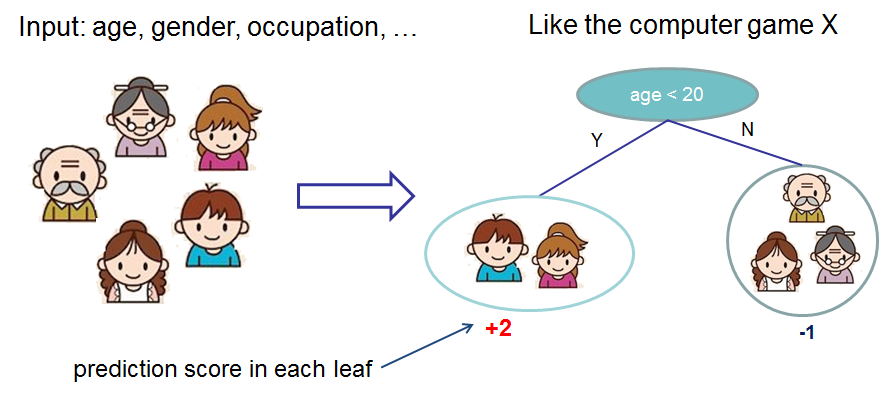
\includegraphics[width=\linewidth]{figures/xgboost_cart_example.png}
    \\[1mm]\small (a) Một cây CART đơn — mỗi hồ sơ nhận điểm dự báo tại lá tương ứng
\end{minipage}
\hfill
\begin{minipage}{0.5\textwidth}
    \centering
    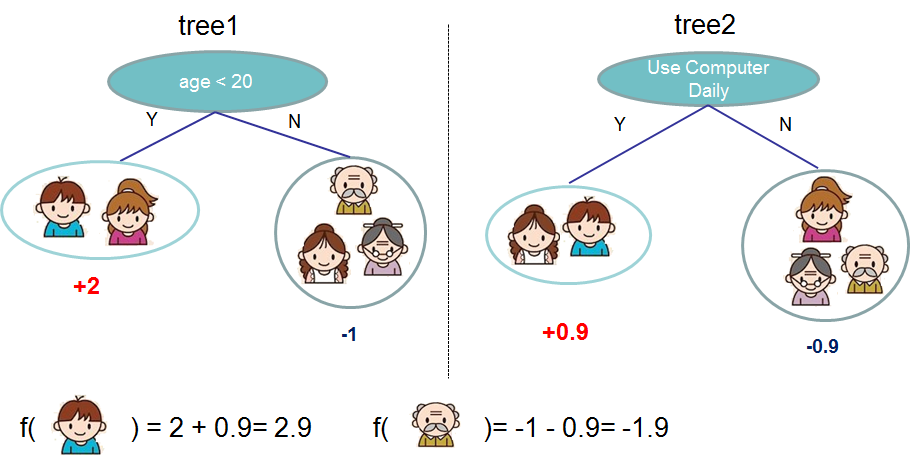
\includegraphics[width=\linewidth]{figures/xgboost_two_trees.png}
    \\[1mm]\small (b) Cộng dồn điểm dự báo của nhiều cây: $f(\mathbf{x})=\sum_t f_t(\mathbf{x})$
\end{minipage}
\caption{Cơ chế cộng dồn các cây trong XGBoost}
\label{fig:xgboost-additive}
\caption*{\textit{Nguồn: Tài liệu chính thức của XGBoost \cite{xgboost_docs}, giấy phép Apache 2.0; minh họa cho cơ chế mô tả trong Chen và Guestrin \cite{chen2016xgboost}; truy cập ngày 15/08/2026.}}
\end{figure}

Hình~\ref{fig:xgboost-additive} thể hiện cách dự báo được cập nhật tuần tự. Mỗi cây mới $f_t(\mathbf{x})$ hiệu chỉnh phần sai số còn lại của tổ hợp trước đó bằng cách cộng thêm điểm số tại lá tương ứng của hồ sơ đang xét, có nhân hệ số học $\eta$; XGBoost đồng thời đưa số hạng chính quy $\Omega(f_t)$ vào hàm mục tiêu để kiểm soát độ phức tạp.

\medskip
\noindent\textbf{LightGBM.}

LightGBM tối ưu tốc độ và bộ nhớ bằng các kỹ thuật như Gradient-based One-Side Sampling và Exclusive Feature Bundling. Thuật toán phát triển cây theo lá tốt nhất, tức là tại mỗi bước ưu tiên tách lá tạo ra mức giảm hàm mất mát lớn nhất. Cách phát triển này có thể hội tụ nhanh nhưng cũng làm cây mất cân đối và dễ quá khớp khi dữ liệu nhỏ; vì vậy cần kiểm soát \mbox{\texttt{num\_leaves}}, \mbox{\texttt{min\_data\_in\_leaf}} và \mbox{\texttt{max\_depth}} \cite{ke2017lightgbm,lightgbm_docs}.

\begin{figure}[H]
\centering
\begin{minipage}{0.48\textwidth}
    \centering
    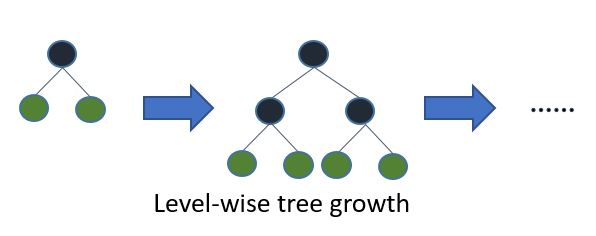
\includegraphics[width=\linewidth]{figures/lightgbm_level_wise.png}
    \\[1mm]\small (a) Phát triển cây theo tầng
\end{minipage}
\hfill
\begin{minipage}{0.48\textwidth}
    \centering
    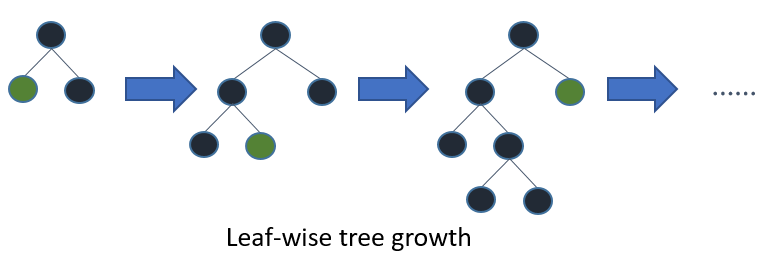
\includegraphics[width=\linewidth]{figures/lightgbm_leaf_wise.png}
    \\[1mm]\small (b) Phát triển cây theo lá tốt nhất
\end{minipage}
\caption{Minh họa hai chiến lược phát triển cây quyết định}
\label{fig:lightgbm-official-growth}
\caption*{\textit{Nguồn: Tài liệu chính thức của LightGBM \cite{lightgbm_docs}, giấy phép MIT; truy cập ngày 15/08/2026.}}
\end{figure}

Hình \ref{fig:lightgbm-official-growth} cho thấy sự khác biệt trực quan giữa hai chiến lược. Phương pháp theo tầng mở rộng đồng thời các nút ở cùng độ sâu và thường tạo ra cấu trúc tương đối cân đối. Ngược lại, LightGBM tiếp tục phân chia lá mang lại mức giảm hàm mất mát lớn nhất, vì vậy cây có thể phát triển không đối xứng. Cơ chế này góp phần nâng cao hiệu quả tối ưu, nhưng đồng thời đòi hỏi kiểm soát độ sâu và số lá để hạn chế hiện tượng quá khớp \cite{ke2017lightgbm,lightgbm_docs}.

\medskip
\noindent\textbf{CatBoost.}

CatBoost có khả năng xử lý trực tiếp biến phân loại và sử dụng cơ chế \textit{ordered boosting} để hạn chế rò rỉ thông tin trong quá trình huấn luyện \cite{prokhorenkova2018catboost}.

\section{Những thách thức khi mô hình hóa dữ liệu tín dụng}

\subsection{Thách thức đối với hiệu năng dự báo}

\noindent\textbf{Mất cân bằng lớp.}
\label{sec:imbalance-theory}

Khi các nhóm nợ có tần suất chênh lệch lớn, mô hình có xu hướng thiên về lớp đa số. Hai hướng xử lý phổ biến, độc lập nhau và có thể kết hợp, là điều chỉnh ở cấp thuật toán (trọng số lớp trong hàm mất mát) và điều chỉnh ở cấp dữ liệu (sinh thêm quan sát tổng hợp cho lớp thiểu số).

\noindent\textit{Cấp thuật toán — trọng số lớp.}
\[
\mathcal{L}
=
-\sum_{i=1}^{N}
w_{y_i}
\sum_{k=1}^{K}
\mathbb{I}(y_i=k)\log p_{ik}.
\]
Trong đó $N$ là số quan sát; $K$ là số lớp; $w_{y_i}$ là trọng số gán cho lớp thật của quan sát $i$; $\mathbb{I}(y_i=k)$ bằng 1 khi $y_i=k$ và bằng 0 trong trường hợp khác; $p_{ik}$ là xác suất dự báo lớp $k$. Trọng số lớn hơn cho lớp hiếm làm sai số của lớp đó có ảnh hưởng lớn hơn tới hàm mất mát. Trọng số thường được tính theo tần suất nghịch đảo:
\[
w_c=\frac{N}{K\,n_c},
\]
trong đó $n_c$ là số quan sát thuộc lớp $c$; mỗi quan sát $i$ được gán trọng số $w_{y_i}$.

\noindent\textit{Cấp dữ liệu — SMOTE.} SMOTE (\textit{Synthetic Minority Over-sampling Technique}) tạo một điểm tổng hợp cho lớp thiểu số bằng nội suy tuyến tính giữa một quan sát và một láng giềng gần cùng lớp:
\[
\mathbf{x}_{\mathrm{new}}
=
\mathbf{x}_i+\lambda\left(\mathbf{x}_{nn}-\mathbf{x}_i\right),
\qquad \lambda\sim U(0,1),
\]
trong đó $\mathbf{x}_i$ là véc-tơ của một quan sát lớp thiểu số; $\mathbf{x}_{nn}$ là một trong các láng giềng gần của nó; $\lambda$ là số ngẫu nhiên phân bố đều trên $[0,1]$; và $\mathbf{x}_{\mathrm{new}}$ là điểm nội suy \cite{chawla2002smote}. Khác với trọng số lớp (không đổi số quan sát, chỉ đổi ảnh hưởng của từng quan sát lên hàm mất mát), SMOTE làm tăng số quan sát huấn luyện của lớp thiểu số bằng dữ liệu nội suy chứ không phải quan sát độc lập mới. Hai hướng có thể dùng riêng hoặc kết hợp; hiệu quả thực tế của từng chiến lược trên dữ liệu của luận văn được đối chiếu thực nghiệm ở Mục~\ref{sec:imbalance} (Chương 2) và Mục~\ref{sec:imbalance-combined-results} (Chương 3).

\medskip
\noindent\textbf{Tính thứ tự.}
Năm nhóm nợ có thứ tự rủi ro từ thấp đến cao nên hai sai số lệch một bậc và lệch bốn bậc không có mức độ nghiêm trọng như nhau. Ordinal MAE, trình bày tại Mục~\ref{sec:metrics} (Chương 3), là một thước đo có thể bổ sung để lượng hóa số bậc sai lệch trung bình. Các bảng thực nghiệm hiện tại chưa báo cáo chỉ tiêu này, nên kết luận về mô hình chưa bao gồm đánh giá định lượng theo thứ tự nhóm nợ.

\subsection{Khả năng giải thích và yêu cầu ứng dụng}
\label{sec:shap-theory}

\[
f(\mathbf{x})=\phi_0+\sum_{j=1}^{p}\phi_j.
\]
Trong đó $f(\mathbf{x})$ là đầu ra mô hình cần giải thích; $\phi_0$ là giá trị nền; $p$ là số đặc trưng; và $\phi_j$ là đóng góp SHAP của đặc trưng $j$ cho hồ sơ $\mathbf{x}$ \cite{lundberg2017unified}.

\begin{figure}[H]
\centering
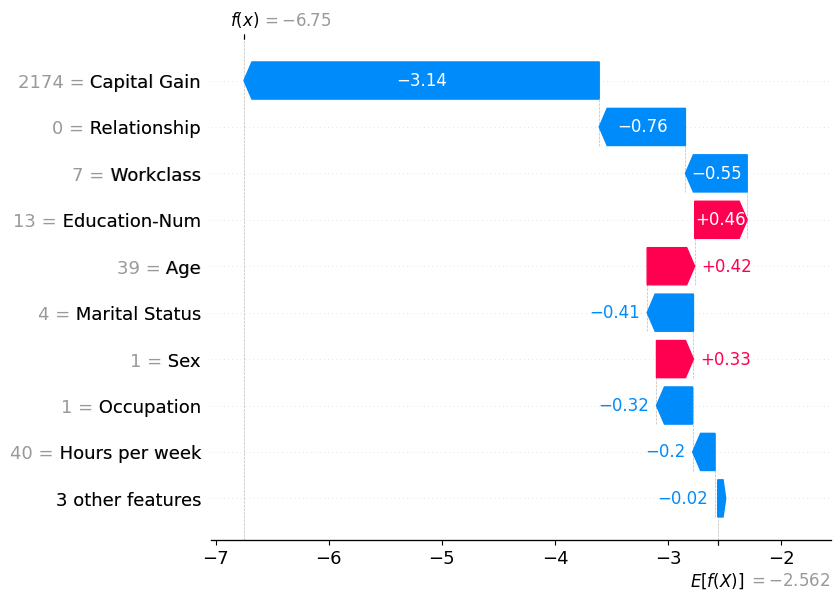
\includegraphics[width=0.72\textwidth]{figures/shap_waterfall_example.png}
\caption{Ví dụ biểu đồ waterfall minh họa nguyên lý phân rã dự báo theo giá trị SHAP}
\label{fig:shap-additive}
\caption*{\textit{Nguồn: Tài liệu chính thức của SHAP \cite{shap_docs}, giấy phép MIT, dựa trên phương pháp của Lundberg và Lee \cite{lundberg2017unified}; truy cập ngày 15/08/2026.}}
\end{figure}

Dự báo theo SHAP bắt đầu từ giá trị nền $\phi_0$ (ký hiệu $E[f(X)]$ trong Hình \ref{fig:shap-additive}), sau đó được điều chỉnh tăng hoặc giảm bởi đóng góp của từng đặc trưng cho tới khi đạt đầu ra $f(\mathbf{x})$ của hồ sơ đang xét. Dấu của $\phi_j$ cho biết chiều tác động đối với đầu ra đang được giải thích (thanh màu đỏ: đóng góp dương; thanh màu xanh: đóng góp âm), còn độ lớn tuyệt đối phản ánh cường độ đóng góp. Hình \ref{fig:shap-additive} chỉ minh họa nguyên lý phân rã từ tài liệu SHAP; các giá trị SHAP thực nghiệm của luận văn được tính riêng trên dữ liệu tín dụng ở Chương 3.

\begin{figure}[H]
\centering
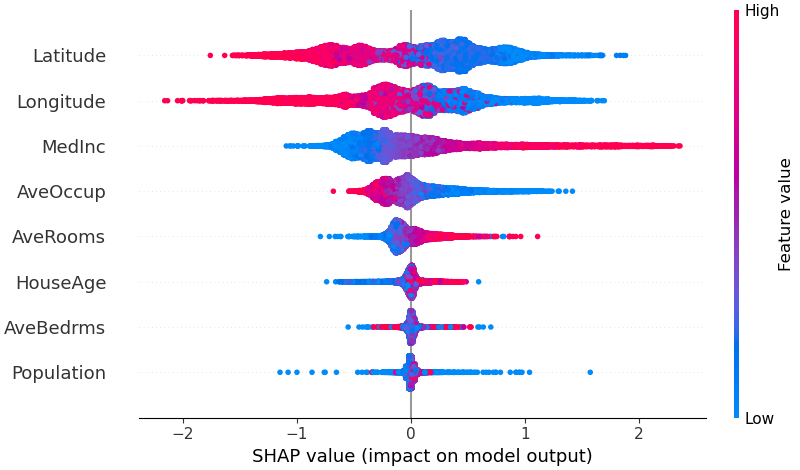
\includegraphics[width=0.82\textwidth]{figures/shap_beeswarm_example.png}
\caption{Ví dụ biểu đồ SHAP beeswarm trong phân tích mức độ tác động của đặc trưng}
\label{fig:shap-official-beeswarm}
\caption*{\textit{Nguồn: Kho tài liệu chính thức của SHAP \cite{shap_docs}, dựa trên phương pháp của Lundberg và Lee \cite{lundberg2017unified}, giấy phép MIT; truy cập ngày 15/08/2026.}}
\end{figure}

Trong biểu đồ beeswarm, mỗi điểm biểu thị một quan sát; vị trí trên trục hoành phản ánh giá trị SHAP, còn màu sắc thể hiện mức độ cao hoặc thấp của giá trị đặc trưng. Các đặc trưng được sắp xếp theo tổng độ lớn ảnh hưởng, qua đó cho phép xem xét đồng thời tầm quan trọng, chiều tác động và mức độ phân tán của ảnh hưởng trên toàn bộ tập dữ liệu. Hình \ref{fig:shap-official-beeswarm} chỉ minh họa cách đọc biểu đồ từ tài liệu SHAP; các kết luận thực nghiệm của luận văn được rút ra từ dữ liệu tín dụng và các biểu đồ được tạo riêng ở Chương 3.

\section{Tóm tắt chương}

Chương này đã trình bày bối cảnh và động lực nghiên cứu xuất phát từ vai trò của hoạt động tín dụng và rủi ro tín dụng trong ngân hàng thương mại, giới hạn hồi cứu của thông tin CIC và căn cứ pháp lý cho yêu cầu về công cụ cảnh báo sớm nội bộ (Mục~\ref{sec:cic-limits}); cơ sở lý thuyết về tín dụng, rủi ro và phân loại nhóm nợ; các mô hình học máy được sử dụng; những thách thức đặc thù của dữ liệu tín dụng; và tổng quan nghiên cứu liên quan làm cơ sở xác định ba khoảng trống nghiên cứu, định vị đề tài và đóng góp dự kiến của luận văn (Mục~\ref{sec:ch1-gaps}). Hệ thống chỉ tiêu đánh giá mô hình được trình bày cùng kết quả thực nghiệm tại Mục~\ref{sec:metrics} (Chương 3).

Trên cơ sở lý thuyết và định hướng đã xác lập, Chương 2 sẽ phát biểu hình thức hai bài toán nghiên cứu và trình bày cụ thể nguồn dữ liệu, quy trình xử lý, phân tích khám phá dữ liệu, xây dựng đặc trưng nghiệp vụ và phương pháp thực nghiệm được cài đặt trong mã nguồn trên hai bộ dữ liệu thực tế của luận văn.


\chapter{CƠ SỞ LÝ THUYẾT VÀ CÁC NGHIÊN CỨU LIÊN QUAN}

Trong chương này, luận văn trình bày nền tảng lý thuyết cần thiết để làm rõ bối cảnh và nội dung của bài toán nghiên cứu. Trước hết, chương giới thiệu các khái niệm về tín dụng, rủi ro tín dụng, phân loại nhóm nợ và tổn thất kỳ vọng. Tiếp theo, chương phân tích sự chuyển dịch từ phương pháp đánh giá truyền thống sang các mô hình học máy, trong đó tập trung vào các thuật toán được sử dụng trong phần thực nghiệm. Những thách thức đặc thù của dữ liệu tín dụng, bao gồm mất cân bằng lớp, tính thứ tự của nhóm nợ, sự thay đổi phân bố theo thời gian và yêu cầu giải thích mô hình, cũng được thảo luận. Cuối cùng, chương trình bày hệ thống chỉ tiêu đánh giá, tổng quan các nghiên cứu liên quan và xác định khoảng trống mà luận văn hướng tới giải quyết. Đây là cơ sở lý luận để xây dựng quy trình nghiên cứu ở Chương 3.

\section{Nền tảng tín dụng, rủi ro và phân loại nhóm nợ}

\subsection{Khái niệm tín dụng và rủi ro tín dụng}

Tín dụng là quan hệ kinh tế trong đó bên cho vay chuyển giao quyền sử dụng một lượng giá trị cho bên đi vay trong một khoảng thời gian xác định, với nghĩa vụ hoàn trả theo các điều kiện đã thỏa thuận.

Rủi ro tín dụng là khả năng phát sinh tổn thất do khách hàng hoặc đối tác không thực hiện đầy đủ nghĩa vụ tài chính. Rủi ro chịu ảnh hưởng từ năng lực tài chính, đặc điểm khoản vay, lịch sử tín dụng, chính sách cấp tín dụng và điều kiện kinh tế.

\subsection{Phân loại nhóm nợ}

\begin{table}[H]
\centering
\caption{Các nhóm nợ trong nghiên cứu}
\begin{tabular}{|c|p{4cm}|p{7cm}|}
\hline
1 & Nợ đủ tiêu chuẩn & Mức rủi ro thấp.\\
\hline
2 & Nợ cần chú ý & Đã xuất hiện dấu hiệu cần theo dõi.\\
\hline
3 & Nợ dưới tiêu chuẩn & Khả năng thu hồi suy giảm đáng kể.\\
\hline
4 & Nợ nghi ngờ & Mức rủi ro cao.\\
\hline
5 & Nợ có khả năng mất vốn & Mức rủi ro cao nhất.\\
\hline
\end{tabular}
\end{table}

\subsection{Xếp hạng tín dụng và tổn thất kỳ vọng}

Xếp hạng tín dụng là quá trình gán khách hàng hoặc khoản vay vào một hạng rủi ro dựa trên thông tin tài chính, đặc điểm khoản vay và lịch sử thực hiện nghĩa vụ. Trong phạm vi luận văn, năm nhóm nợ được xem là các mức rủi ro có thứ tự; mô hình được xây dựng để hỗ trợ nhận diện nhóm nợ tương ứng của từng quan sát.

Tổn thất kỳ vọng có thể biểu diễn:
\[
EL=PD\times LGD\times EAD.
\]
Trong đó $EL$ là tổn thất kỳ vọng; $PD$ là xác suất vỡ nợ trong kỳ đánh giá; $LGD$ là tỷ lệ tổn thất khi vỡ nợ sau khi xét khả năng thu hồi; và $EAD$ là dư nợ tại thời điểm vỡ nợ. Luận văn hiện tập trung vào phân loại trạng thái rủi ro, chưa trực tiếp ước lượng đủ ba cấu phần của $EL$ \cite{basel_framework}.

\begin{figure}[H]
\centering
\begin{tikzpicture}[
    >=stealth,
    font=\small,
    riskbox/.style={draw, rounded corners=2pt, align=center, minimum height=1.8cm, text width=3.7cm},
    resultbox/.style={draw, rounded corners=2pt, very thick, align=center, minimum height=1.45cm, text width=4.2cm}
]
    \node[riskbox] (pd) at (-5.0,1.6)
        {\textbf{$PD$}\\Xác suất khách hàng vỡ nợ trong kỳ đánh giá};
    \node[riskbox] (lgd) at (0,1.6)
        {\textbf{$LGD$}\\Tỷ lệ tổn thất sau khi xét phần có thể thu hồi};
    \node[riskbox] (ead) at (5.0,1.6)
        {\textbf{$EAD$}\\Dư nợ của khoản cấp tín dụng tại thời điểm vỡ nợ};
    \node[resultbox] (el) at (0,-1.25)
        {\textbf{Tổn thất kỳ vọng}\\$EL=PD\times LGD\times EAD$};
    \draw[->, very thick] (pd.south) -- (el.north west);
    \draw[->, very thick] (lgd.south) -- (el.north);
    \draw[->, very thick] (ead.south) -- (el.north east);
\end{tikzpicture}
\caption{Các cấu phần của tổn thất kỳ vọng trong rủi ro tín dụng}
\label{fig:el-components}
\caption*{\textit{Nguồn: Tác giả tổng hợp và vẽ lại từ Basel Committee on Banking Supervision \cite{basel_framework}.}}
\end{figure}

\section{Từ đánh giá truyền thống đến các mô hình học máy}

\subsection{Sự chuyển dịch từ phương pháp truyền thống sang học máy}

Phương pháp chuyên gia có khả năng khai thác thông tin định tính nhưng chủ quan. Z-score của Altman có ý nghĩa nền tảng nhưng phụ thuộc dữ liệu kế toán và quan hệ tuyến tính. Logistic Regression dễ giải thích nhưng khó tự động nắm bắt tương tác phức tạp.

Học máy là nhánh của AI trong đó mô hình học quy luật từ dữ liệu. Bài toán của luận văn thuộc học có giám sát.

\subsection{Mô hình tuyến tính và cây quyết định}

\noindent\textbf{Logistic Regression đa lớp.}

\[
P(Y=k\mid\mathbf{x})
=
\frac{\exp(\beta_{k0}+\boldsymbol{\beta}_{k}^{T}\mathbf{x})}
{\sum_{j=1}^{K}\exp(\beta_{j0}+\boldsymbol{\beta}_{j}^{T}\mathbf{x})}.
\]
Trong đó $K$ là số lớp; $\mathbf{x}$ là véc-tơ đặc trưng; $\beta_{k0}$ là hệ số chặn của lớp $k$; $\boldsymbol{\beta}_{k}$ là véc-tơ hệ số của lớp $k$; và mẫu số chuẩn hóa để tổng xác suất của $K$ lớp bằng 1 \cite{hosmer2013applied}.

\medskip
\noindent\textbf{Decision Tree.}

Decision Tree chia không gian đặc trưng bằng các điều kiện dạng $x_j\le s$. Mô hình dễ giải thích nhưng dễ overfitting.

\medskip
\noindent\textbf{Random Forest.}

\[
\hat{y}=\operatorname{mode}\{h_b(\mathbf{x})\}_{b=1}^{B}.
\]
Trong đó $B$ là số cây; $h_b(\mathbf{x})$ là dự báo lớp của cây thứ $b$ tại hồ sơ $\mathbf{x}$; và $\operatorname{mode}$ chọn lớp xuất hiện nhiều nhất trong các dự báo cây \cite{breiman2001random}.

\subsection{Các mô hình boosting}

\noindent\textbf{XGBoost.}

\[
\mathcal{L}^{(t)}
=
\sum_{i=1}^{n}
l(y_i,\hat{y}_{i}^{(t-1)}+f_t(\mathbf{x}_i))
+\Omega(f_t).
\]
Trong đó $t$ là vòng boosting; $n$ là số quan sát huấn luyện; $l(\cdot)$ là hàm mất mát; $\hat{y}_{i}^{(t-1)}$ là dự báo tích lũy trước vòng $t$; $f_t$ là cây mới; và $\Omega(f_t)$ là số hạng phạt độ phức tạp của cây nhằm hạn chế quá khớp \cite{chen2016xgboost}.

\begin{figure}[H]
\centering
\begin{minipage}{0.46\textwidth}
    \centering
    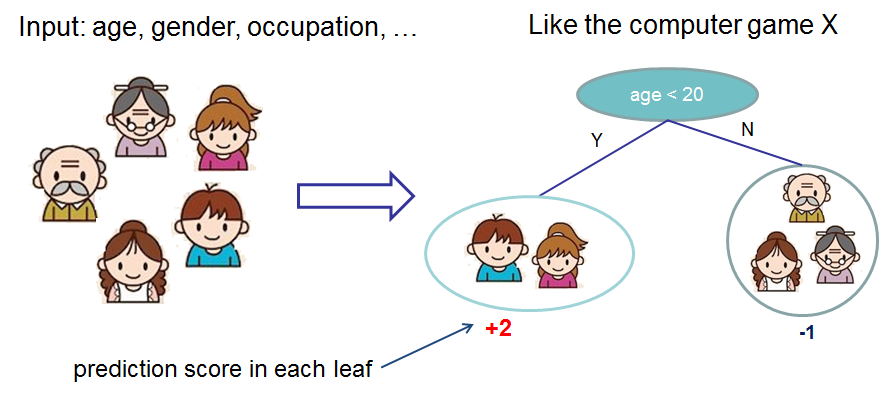
\includegraphics[width=\linewidth]{figures/xgboost_cart_example.png}
    \\[1mm]\small (a) Một cây CART đơn — mỗi hồ sơ nhận điểm dự báo tại lá tương ứng
\end{minipage}
\hfill
\begin{minipage}{0.5\textwidth}
    \centering
    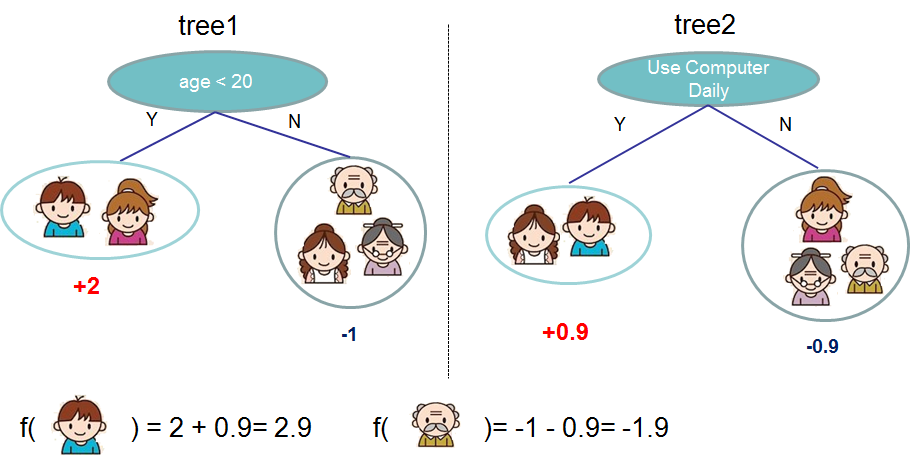
\includegraphics[width=\linewidth]{figures/xgboost_two_trees.png}
    \\[1mm]\small (b) Cộng dồn điểm dự báo của nhiều cây: $f(\mathbf{x})=\sum_t f_t(\mathbf{x})$
\end{minipage}
\caption{Cơ chế cộng dồn các cây trong XGBoost}
\label{fig:xgboost-additive}
\caption*{\textit{Nguồn: Tài liệu chính thức của XGBoost \cite{xgboost_docs}, giấy phép Apache 2.0; minh họa cho cơ chế mô tả trong Chen và Guestrin \cite{chen2016xgboost}; truy cập ngày 15/08/2026.}}
\end{figure}

Hình~\ref{fig:xgboost-additive} thể hiện cách dự báo được cập nhật tuần tự. Mỗi cây mới $f_t(\mathbf{x})$ hiệu chỉnh phần sai số còn lại của tổ hợp trước đó bằng cách cộng thêm điểm số tại lá tương ứng của hồ sơ đang xét, có nhân hệ số học $\eta$; XGBoost đồng thời đưa số hạng chính quy $\Omega(f_t)$ vào hàm mục tiêu để kiểm soát độ phức tạp.

\medskip
\noindent\textbf{LightGBM.}

LightGBM tối ưu tốc độ và bộ nhớ bằng các kỹ thuật như Gradient-based One-Side Sampling và Exclusive Feature Bundling. Thuật toán phát triển cây theo lá tốt nhất, tức là tại mỗi bước ưu tiên tách lá tạo ra mức giảm hàm mất mát lớn nhất. Cách phát triển này có thể hội tụ nhanh nhưng cũng làm cây mất cân đối và dễ quá khớp khi dữ liệu nhỏ; vì vậy cần kiểm soát \mbox{\texttt{num\_leaves}}, \mbox{\texttt{min\_data\_in\_leaf}} và \mbox{\texttt{max\_depth}} \cite{ke2017lightgbm,lightgbm_docs}.

\begin{figure}[H]
\centering
\begin{minipage}{0.48\textwidth}
    \centering
    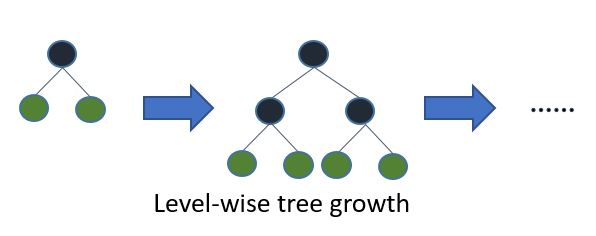
\includegraphics[width=\linewidth]{figures/lightgbm_level_wise.png}
    \\[1mm]\small (a) Phát triển cây theo tầng
\end{minipage}
\hfill
\begin{minipage}{0.48\textwidth}
    \centering
    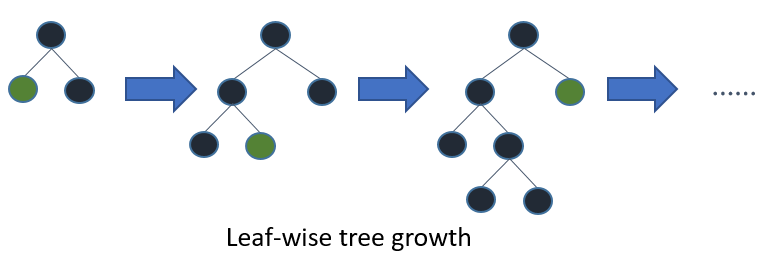
\includegraphics[width=\linewidth]{figures/lightgbm_leaf_wise.png}
    \\[1mm]\small (b) Phát triển cây theo lá tốt nhất
\end{minipage}
\caption{Minh họa hai chiến lược phát triển cây quyết định}
\label{fig:lightgbm-official-growth}
\caption*{\textit{Nguồn: Tài liệu chính thức của LightGBM \cite{lightgbm_docs}, giấy phép MIT; truy cập ngày 15/08/2026.}}
\end{figure}

Hình \ref{fig:lightgbm-official-growth} cho thấy sự khác biệt trực quan giữa hai chiến lược. Phương pháp theo tầng mở rộng đồng thời các nút ở cùng độ sâu và thường tạo ra cấu trúc tương đối cân đối. Ngược lại, LightGBM tiếp tục phân chia lá mang lại mức giảm hàm mất mát lớn nhất, vì vậy cây có thể phát triển không đối xứng. Cơ chế này góp phần nâng cao hiệu quả tối ưu, nhưng đồng thời đòi hỏi kiểm soát độ sâu và số lá để hạn chế hiện tượng quá khớp \cite{ke2017lightgbm,lightgbm_docs}.

\medskip
\noindent\textbf{CatBoost.}

CatBoost có khả năng xử lý trực tiếp biến phân loại và sử dụng cơ chế \textit{ordered boosting} để hạn chế rò rỉ thông tin trong quá trình huấn luyện \cite{prokhorenkova2018catboost}.

\section{Những thách thức khi mô hình hóa dữ liệu tín dụng}

\subsection{Thách thức đối với hiệu năng dự báo}

\noindent\textbf{Mất cân bằng lớp.}

\[
\mathcal{L}
=
-\sum_{i=1}^{N}
w_{y_i}
\sum_{k=1}^{K}
\mathbb{I}(y_i=k)\log p_{ik}.
\]
Trong đó $N$ là số quan sát; $K$ là số lớp; $w_{y_i}$ là trọng số gán cho lớp thật của quan sát $i$; $\mathbb{I}(y_i=k)$ bằng 1 khi $y_i=k$ và bằng 0 trong trường hợp khác; $p_{ik}$ là xác suất dự báo lớp $k$. Trọng số lớn hơn cho lớp hiếm làm sai số của lớp đó có ảnh hưởng lớn hơn tới hàm mất mát.

\medskip
\noindent\textbf{Tính thứ tự.}
Năm nhóm nợ có thứ tự rủi ro từ thấp đến cao nên hai sai số lệch một bậc và lệch bốn bậc không có mức độ nghiêm trọng như nhau. Luận văn sử dụng Ordinal MAE ở phần chỉ tiêu đánh giá để lượng hóa số bậc sai lệch trung bình; chỉ tiêu này chưa được hàm \mbox{\texttt{compute\_metrics()}} của mã nguồn báo cáo trong kết quả chính.

\subsection{Khả năng giải thích và yêu cầu ứng dụng}
\label{sec:shap-theory}

\[
f(\mathbf{x})=\phi_0+\sum_{j=1}^{p}\phi_j.
\]
Trong đó $f(\mathbf{x})$ là đầu ra mô hình cần giải thích; $\phi_0$ là giá trị nền; $p$ là số đặc trưng; và $\phi_j$ là đóng góp SHAP của đặc trưng $j$ cho hồ sơ $\mathbf{x}$ \cite{lundberg2017unified}.

\begin{figure}[H]
\centering
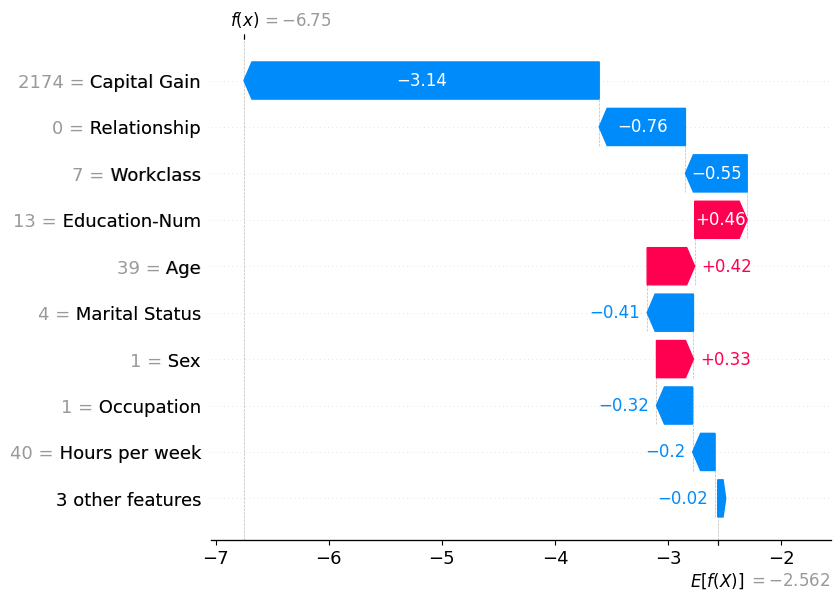
\includegraphics[width=0.72\textwidth]{figures/shap_waterfall_example.png}
\caption{Ví dụ biểu đồ waterfall minh họa nguyên lý phân rã dự báo theo giá trị SHAP}
\label{fig:shap-additive}
\caption*{\textit{Nguồn: Tài liệu chính thức của SHAP \cite{shap_docs}, giấy phép MIT, dựa trên phương pháp của Lundberg và Lee \cite{lundberg2017unified}; truy cập ngày 15/08/2026.}}
\end{figure}

Dự báo theo SHAP bắt đầu từ giá trị nền $\phi_0$ (ký hiệu $E[f(X)]$ trong Hình \ref{fig:shap-additive}), sau đó được điều chỉnh tăng hoặc giảm bởi đóng góp của từng đặc trưng cho tới khi đạt đầu ra $f(\mathbf{x})$ của hồ sơ đang xét. Dấu của $\phi_j$ cho biết chiều tác động đối với đầu ra đang được giải thích (thanh màu đỏ: đóng góp dương; thanh màu xanh: đóng góp âm), còn độ lớn tuyệt đối phản ánh cường độ đóng góp. Hình \ref{fig:shap-additive} chỉ minh họa nguyên lý phân rã từ tài liệu SHAP; các giá trị SHAP thực nghiệm của luận văn được tính riêng trên dữ liệu tín dụng ở Chương 4.

\begin{figure}[H]
\centering
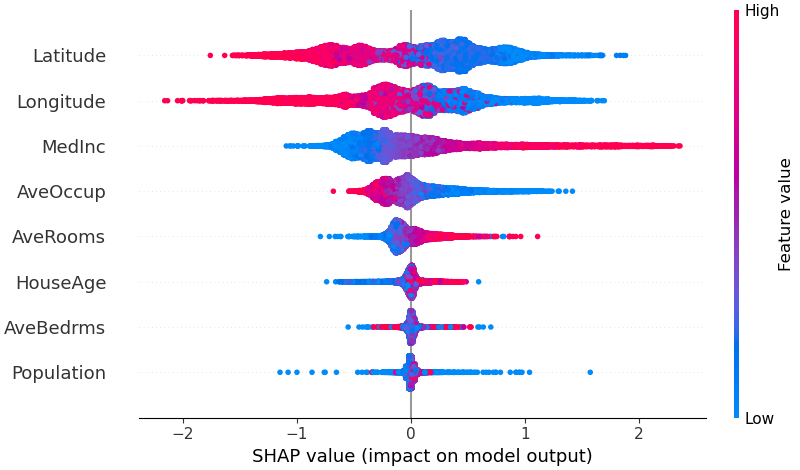
\includegraphics[width=0.82\textwidth]{figures/shap_beeswarm_example.png}
\caption{Ví dụ biểu đồ SHAP beeswarm trong phân tích mức độ tác động của đặc trưng}
\label{fig:shap-official-beeswarm}
\caption*{\textit{Nguồn: Kho tài liệu chính thức của SHAP \cite{shap_docs}, dựa trên phương pháp của Lundberg và Lee \cite{lundberg2017unified}, giấy phép MIT; truy cập ngày 15/08/2026.}}
\end{figure}

Trong biểu đồ beeswarm, mỗi điểm biểu thị một quan sát; vị trí trên trục hoành phản ánh giá trị SHAP, còn màu sắc thể hiện mức độ cao hoặc thấp của giá trị đặc trưng. Các đặc trưng được sắp xếp theo tổng độ lớn ảnh hưởng, qua đó cho phép xem xét đồng thời tầm quan trọng, chiều tác động và mức độ phân tán của ảnh hưởng trên toàn bộ tập dữ liệu. Hình \ref{fig:shap-official-beeswarm} chỉ minh họa cách đọc biểu đồ từ tài liệu SHAP; các kết luận thực nghiệm của luận văn được rút ra từ dữ liệu tín dụng và các biểu đồ được tạo riêng ở Chương 4.

\section{Hệ thống chỉ tiêu đánh giá mô hình}

\subsection{Chỉ tiêu tổng thể và theo lớp}

\noindent\textbf{Accuracy.}
\[
Accuracy=
\frac{\sum_{k=1}^{K}C_{kk}}
{\sum_{i=1}^{K}\sum_{j=1}^{K}C_{ij}}.
\]
Trong đó $C_{ij}$ là số quan sát có lớp thật $i$ và lớp dự báo $j$; tử số là tổng phần tử đường chéo; mẫu số là tổng số quan sát.

\medskip
\noindent\textbf{Precision, Recall và F1.}
\[
Precision_k=\frac{TP_k}{TP_k+FP_k},
\qquad
Recall_k=\frac{TP_k}{TP_k+FN_k},
\]
Trong đó $TP_k$ là số dự báo đúng lớp $k$; $FP_k$ là số quan sát lớp khác bị dự báo nhầm thành $k$; và $FN_k$ là số quan sát lớp $k$ bị dự báo sang lớp khác.
\[
F1_k=2\frac{Precision_k\times Recall_k}{Precision_k+Recall_k}.
\]

\subsection{Chỉ tiêu cho dữ liệu mất cân bằng}

\noindent\textbf{Macro F1.}
\[
F1_{\mathrm{macro}}=\frac{1}{K}\sum_{k=1}^{K}F1_k.
\]

\medskip
\noindent\textbf{Weighted F1.}
\[
F1_{\mathrm{weighted}}=\sum_{k=1}^{K}\frac{n_k}{N}F1_k.
\]
Trong đó $n_k$ là số quan sát thật của lớp $k$ và $N$ là tổng số quan sát. Khi một lớp chiếm tỷ trọng rất lớn, Weighted-F1 có thể che khuất hiệu năng thấp của lớp hiếm.

\medskip
\noindent\textbf{Balanced Accuracy.}
\[
Balanced\ Accuracy=\frac{1}{K}\sum_{k=1}^{K}Recall_k.
\]
Balanced Accuracy là trung bình Recall của $K$ lớp, nên mỗi lớp có trọng số như nhau bất kể tần suất.

\subsection{Chỉ tiêu phản ánh thứ tự nhóm nợ}

\noindent\textbf{Ordinal MAE.}
\[
Ordinal\ MAE=\frac{1}{N}\sum_{i=1}^{N}|y_i-\hat{y}_i|.
\]
Ký hiệu có ý nghĩa như phần Tính thứ tự; giá trị càng nhỏ thì khoảng cách nhóm dự báo so với nhóm thật càng thấp.

\section{Nghiên cứu liên quan, khoảng trống và định hướng}

\subsection{Kết quả chính của các nghiên cứu liên quan}

Hand và Henley \cite{hand1997statistical} hệ thống hóa các phương pháp phân loại thống kê; Thomas \cite{thomas2000survey} mở rộng phạm vi từ đánh giá tại thời điểm phê duyệt sang theo dõi hành vi trong vòng đời khoản vay. Baesens và cộng sự \cite{baesens2003benchmarking} và Lessmann và cộng sự \cite{lessmann2015benchmarking} cho thấy hiệu quả mô hình phụ thuộc vào dữ liệu, thước đo và quy trình đánh giá.

Brown và Mues \cite{brown2012experimental} nhấn mạnh ảnh hưởng của mất cân bằng. Xia và cộng sự \cite{xia2017boosted} cho thấy boosted tree có khả năng cải thiện dự báo. Barboza và cộng sự \cite{barboza2017machine} ghi nhận kết quả cạnh tranh của các mô hình cây trong dự báo phá sản. Dastile và cộng sự \cite{dastile2020statistical} chỉ ra các hạn chế phổ biến về dữ liệu nhỏ, mất cân bằng, thiếu chuẩn đánh giá và khả năng giải thích.

Tại Việt Nam, nghiên cứu thường tập trung vào đánh giá rủi ro tín dụng cá nhân, rủi ro doanh nghiệp và dự báo nợ xấu. Tuy nhiên, chưa có nhiều nghiên cứu công bố việc phân loại trực tiếp năm nhóm nợ trên dữ liệu thực tế, kết hợp so sánh nhiều mô hình, chia dữ liệu theo thời gian, đánh giá có xét thứ tự và phân tích khả năng giải thích.

\subsection{Khoảng trống và định hướng của luận văn}

\begin{enumerate}
    \item Phần lớn nghiên cứu dùng mục tiêu nhị phân.
    \item Tính thứ tự của năm nhóm nợ chưa được khai thác đầy đủ.
    \item Dữ liệu thực tế tại ngân hàng Việt Nam ít được công bố.
    \item Phương pháp chia mẫu ngẫu nhiên vẫn được sử dụng phổ biến hơn phương pháp chia mẫu theo thời gian.
    \item Lớp rủi ro cao ít quan sát nhưng chưa được đánh giá đầy đủ.
    \item Mô hình phức tạp thường thiếu khả năng giải thích.
\end{enumerate}

\medskip
\noindent\textbf{Định hướng nghiên cứu.}
Luận văn xây dựng bài toán phân loại năm nhóm nợ, kiểm tra và hình thành các đặc trưng nghiệp vụ, sử dụng Logistic Regression làm mô hình cơ sở để đối chiếu với các mô hình cây và mô hình tăng cường, đồng thời xử lý mất cân bằng lớp, đánh giá bằng hệ thống chỉ tiêu đa lớp và giải thích mô hình thông qua mức độ quan trọng của đặc trưng cùng SHAP. Thực nghiệm hiện tại sử dụng phép chia ngẫu nhiên có phân tầng; phép chia theo thời gian là yêu cầu cần thiết trong giai đoạn xây dựng nhãn chuyển nhóm nợ.

\section{Tóm tắt chương}

Chương này đã trình bày cơ sở lý thuyết, thành tựu và hạn chế của các công trình nền tảng, các mô hình được sử dụng, các vấn đề đặc thù của dữ liệu tín dụng, hệ thống chỉ tiêu đánh giá, tổng quan nghiên cứu, khoảng trống và định hướng của luận văn.

Trên cơ sở lý thuyết và định hướng đã xác lập, Chương 3 sẽ trình bày cụ thể nguồn dữ liệu, quy trình xử lý, phân tích khám phá dữ liệu, xây dựng đặc trưng nghiệp vụ và phương pháp thực nghiệm được cài đặt trong mã nguồn trên hai bộ dữ liệu thực tế của luận văn.


\chapter{DỮ LIỆU VÀ PHƯƠNG PHÁP NGHIÊN CỨU}

Chương này trình bày thiết kế nghiên cứu và cách thức triển khai thực nghiệm trên hai bộ dữ liệu tín dụng. Trước hết, chương xác định phạm vi của bài toán, mô tả nguồn dữ liệu và giới thiệu các công nghệ được sử dụng để xây dựng hệ thống. Tiếp theo, quy trình nghiên cứu được trình bày theo các bước từ phân tích khám phá, làm sạch và tiền xử lý dữ liệu đến xây dựng đặc trưng, kiểm soát rò rỉ thông tin và xử lý mất cân bằng lớp. Phần cuối của chương mô tả phương pháp chia mẫu, huấn luyện, hiệu chỉnh, triển khai và giám sát mô hình. Cách tổ chức này nhằm bảo đảm sự liên kết giữa cơ sở lý thuyết ở Chương 2 với quy trình tạo ra các kết quả thực nghiệm được phân tích ở Chương 4.

\section{Định hướng và phạm vi thực nghiệm}

Nguồn dữ liệu gồm hai bộ dữ liệu chứa thông tin đã được mã hóa về các khoản vay tại ngân hàng thương mại thuộc phạm vi nghiên cứu. Bộ dữ liệu A, \path{Data_credit_rating_VN.xlsx}, gồm 27.001 quan sát và 21 biến ban đầu; biến đích \mbox{\texttt{NHOMNOMOI}} nhận giá trị từ 1 đến 5, tương ứng với năm nhóm nợ. Bộ dữ liệu B được trích xuất từ hai kỳ báo cáo liên tiếp của cùng một tổ chức tín dụng: \texttt{Thông tin tín dụng 20260430.xlsx} (100.617 hợp đồng và 41 cột thô, dùng để huấn luyện và kiểm định nội bộ) và \texttt{Thông tin tín dụng 20260507.xlsx} (100.274 hợp đồng và 33 cột thô, dùng làm \emph{tập kiểm tra độc lập}, hoàn toàn tách biệt khỏi quá trình huấn luyện). Biến đích \texttt{Nhóm nợ tự phân loại} cũng nhận giá trị từ 1 đến 5. Do tập dữ liệu kỳ 20260507 chỉ chứa 33 trong tổng số 41 cột của kỳ 20260430, tập đặc trưng của bộ B chỉ được xây dựng từ các cột hiện diện ở cả hai kỳ. Ràng buộc này bảo đảm rằng mô hình được huấn luyện trên kỳ 20260430 có thể áp dụng cho kỳ 20260507 (Mục \ref{sec:pool-a}).

Phạm vi thực nghiệm của luận văn gồm hai bài toán có mục tiêu khác nhau. Bài toán thứ nhất phân loại trạng thái hiện tại của khoản vay vào một trong năm nhóm nợ trên hai bộ dữ liệu A và B. Bài toán thứ hai dự báo khả năng khoản vay chuyển sang nhóm nợ có mức rủi ro cao hơn trong tháng kế tiếp, được xây dựng bằng cách ghép hai kỳ báo cáo liên tiếp của bộ B. Bài toán thứ hai hướng trực tiếp tới mục tiêu hỗ trợ cảnh báo sớm, trong khi bài toán thứ nhất được sử dụng để đối sánh phương pháp mô hình hóa, đánh giá vai trò của các nhóm đặc trưng và kiểm tra khả năng tổng quát hóa ngoài mẫu.

Nếu có dữ liệu bảng theo thời gian, nhãn chuyển nhóm cần được định nghĩa:
\[
Y_{i,t}^{(h)}
=
\begin{cases}
1, & G_{i,t+h}>G_{i,t},\\
0, & G_{i,t+h}\leq G_{i,t},
\end{cases}
\]
trong đó $i$ biểu thị khoản vay hoặc khách hàng; $t$ là thời điểm quan sát; $h$ là khoảng dự báo; $G_{i,t}\in\{1,2,3,4,5\}$ là nhóm nợ tại thời điểm $t$; và $Y_{i,t}^{(h)}=1$ biểu thị sự chuyển dịch sang nhóm có mức rủi ro cao hơn trong khoảng $h$. Trong thực nghiệm trên bộ B, luận văn sử dụng hai kỳ báo cáo liên tiếp và xác định $h=1$ tháng. Toàn bộ đặc trưng đầu vào được lấy tại thời điểm $t$, còn trạng thái tại $t+h$ chỉ được sử dụng để xây dựng nhãn, qua đó hạn chế nguy cơ rò rỉ thông tin từ tương lai.

\section{Quy trình nghiên cứu tổng thể}
\label{sec:pipeline-overview}

Quy trình thực nghiệm được tổ chức thành bảy bước tuần tự, thể hiện tại Hình \ref{fig:experimental-pipeline}: (1) thu thập dữ liệu gốc; (2) phân tích khám phá và làm sạch dữ liệu; (3) tiền xử lý và lựa chọn biến, bao gồm tính WOE/IV, mã hóa và chuẩn hóa; (4) phân chia tập huấn luyện--kiểm định và xử lý mất cân bằng lớp; (5) huấn luyện mô hình; (6) đánh giá hiệu quả và giải thích kết quả; và (7) rút ra kết luận cùng khuyến nghị ứng dụng. Cấu trúc này góp phần hạn chế ảnh hưởng của dữ liệu kiểm định đối với quá trình huấn luyện và phù hợp với nguyên tắc đánh giá ngoài mẫu trong học máy \cite{bishop2006pattern,lessmann2015benchmarking}.

\begin{figure}[H]
\centering
\begin{tabular}{c}
\fbox{\parbox[c][1.5cm][c]{9.6cm}{\centering \textbf{1. Thu thập dữ liệu}\\\footnotesize Khoản vay, khách hàng, lịch sử trả nợ}}\\[1mm]
$\Downarrow$\\[1mm]
\fbox{\parbox[c][1.5cm][c]{9.6cm}{\centering \textbf{2. EDA \& làm sạch dữ liệu}\\\footnotesize Giá trị thiếu, ngoại lệ, phân phối}}\\[1mm]
$\Downarrow$\\[1mm]
\fbox{\parbox[c][1.5cm][c]{9.6cm}{\centering \textbf{3. Tiền xử lý \& chọn biến}\\\footnotesize WOE/IV, mã hóa, chuẩn hóa}}\\[1mm]
$\Downarrow$\\[1mm]
\fbox{\parbox[c][1.5cm][c]{9.6cm}{\centering \textbf{4. Chia dữ liệu \& cân bằng lớp}\\\footnotesize Train/test, SMOTE, class weight}}\\[1mm]
$\Downarrow$\\[1mm]
\fbox{\parbox[c][1.5cm][c]{9.6cm}{\centering \textbf{5. Huấn luyện mô hình}\\\footnotesize LR, RF, XGBoost, LightGBM\ldots}}\\[1mm]
$\Downarrow$\\[1mm]
\fbox{\parbox[c][1.5cm][c]{9.6cm}{\centering \textbf{6. Đánh giá \& giải thích}\\\footnotesize F1, AUC, ma trận nhầm lẫn, SHAP}}\\[1mm]
$\Downarrow$\\[1mm]
\fbox{\parbox[c][1.5cm][c]{9.6cm}{\centering \textbf{7. Kết luận \& ứng dụng}\\\footnotesize Cảnh báo sớm, khuyến nghị}}\\
\end{tabular}
\caption{Pipeline nghiên cứu tổng thể — từ thu thập dữ liệu tới kết luận và ứng dụng}
\label{fig:experimental-pipeline}
\end{figure}

\section{Công nghệ và môi trường triển khai}
\label{sec:technologies}

Toàn bộ quy trình thực nghiệm và ứng dụng minh họa được xây dựng bằng Python 3.11. Ngôn ngữ này được lựa chọn nhờ hệ sinh thái thư viện tương đối hoàn chỉnh cho xử lý dữ liệu, học máy, giải thích mô hình và phát triển ứng dụng tương tác. Các công nghệ chính được tổng hợp tại Bảng \ref{tab:technologies}. Danh sách này được xác định từ tệp \texttt{requirements.txt} và các mô-đun được sử dụng trực tiếp trong mã nguồn của nghiên cứu.

\begin{table}[H]
\centering
\caption{Các công nghệ chính được sử dụng trong nghiên cứu}
\label{tab:technologies}
\begin{tabular}{|p{3.4cm}|p{4.0cm}|p{6.3cm}|}
\hline
\textbf{Công nghệ} & \textbf{Vai trò} & \textbf{Nội dung sử dụng trong luận văn}\\
\hline
Python 3.11 & Ngôn ngữ lập trình & Tổ chức quy trình xử lý dữ liệu, huấn luyện, đánh giá, lưu trữ và phục vụ mô hình.\\
\hline
pandas, NumPy & Xử lý và tính toán dữ liệu & Đọc dữ liệu Excel, biến đổi bảng dữ liệu, xử lý giá trị thiếu, xây dựng đặc trưng và thực hiện các phép tính ma trận.\\
\hline
scikit-learn & Học máy và đánh giá & Xây dựng Logistic Regression, Decision Tree, Random Forest, quy trình tiền xử lý, chia mẫu và tính các chỉ tiêu đánh giá.\\
\hline
imbalanced-learn & Xử lý mất cân bằng lớp & Xây dựng quy trình có SMOTE, BorderlineSMOTE, ADASYN, SMOTETomek và lấy mẫu dưới ngẫu nhiên.\\
\hline
XGBoost, LightGBM, CatBoost & Mô hình boosting & Huấn luyện và đối sánh ba họ mô hình tăng cường dựa trên cây quyết định.\\
\hline
SHAP & Giải thích mô hình & Ước lượng đóng góp của đặc trưng ở phạm vi toàn cục, theo nhóm nghiệp vụ và đối với từng quan sát.\\
\hline
Plotly, Matplotlib & Trực quan hóa & Biểu diễn phân bố dữ liệu, ma trận nhầm lẫn, đường cong hiệu năng và mức độ quan trọng của đặc trưng.\\
\hline
Streamlit & Ứng dụng minh họa & Xây dựng giao diện phân tích khám phá, huấn luyện, chấm điểm, dự báo và so sánh mô hình.\\
\hline
OpenPyXL, Pickle & Trao đổi và lưu trữ & Đọc--ghi tệp Excel và tuần tự hóa mô hình đã huấn luyện để tái sử dụng trong ứng dụng.\\
\hline
\end{tabular}
\end{table}

Về kiến trúc, lớp dữ liệu được quản lý bằng pandas và NumPy; lớp mô hình hóa được triển khai trên scikit-learn, imbalanced-learn cùng ba thư viện boosting; lớp giải thích và trực quan hóa sử dụng SHAP, Plotly và Matplotlib; trong khi Streamlit đảm nhiệm lớp giao diện. Cách phân tách này giúp các bước tiền xử lý, huấn luyện và đánh giá được tái sử dụng thống nhất giữa các chức năng của ứng dụng.

\section{Bước 1: Thu thập dữ liệu}
\label{sec:step1-collect}

Bước đầu tiên của quy trình gồm thu thập và kiểm tra hai tệp dữ liệu gốc, xác định biến đích và khảo sát sơ bộ phân bố nhóm nợ trước khi thực hiện các bước xử lý tiếp theo.

\subsection{Bộ dữ liệu A: Data\_credit\_rating\_VN}
\label{sec:dataset-a-structure}

Bộ dữ liệu A gồm 27.001 hợp đồng vay và không có bản ghi thiếu dữ liệu tại biến đích \mbox{\texttt{NHOMNOMOI}}. Theo Bảng \ref{tab:dataset-a-distribution}, nhóm 1 chiếm 77,65\%, trong khi nhóm 3 chỉ chiếm 2,24\%, cho thấy phân bố nhóm nợ có mức độ mất cân bằng đáng kể.

\begin{table}[H]
\centering
\caption{Phân bố năm nhóm nợ trong bộ dữ liệu A}
\label{tab:dataset-a-distribution}
\begin{tabular}{|c|r|r|r|r|}
\hline
Nhóm & Toàn bộ & Tỷ lệ (\%) & Huấn luyện & Kiểm định\\
\hline
1 & 20.965 & 77,65 & 16.771 & 4.194\\
2 & 1.287 & 4,77 & 1.030 & 257\\
3 & 604 & 2,24 & 483 & 121\\
4 & 784 & 2,90 & 627 & 157\\
5 & 3.361 & 12,45 & 2.689 & 672\\
\hline
Tổng & 27.001 & 100,00 & 21.600 & 5.401\\
\hline
\end{tabular}
\end{table}

\subsection{Bộ dữ liệu B: Thông tin tín dụng}
\label{sec:dataset-b-structure}

Bộ dữ liệu B gồm 100.617 hợp đồng vay ở kỳ báo cáo 20260430 và không có bản ghi thiếu dữ liệu tại biến đích \texttt{Nhóm nợ tự phân loại}. Theo Bảng \ref{tab:split-distribution}, tỷ lệ giữa nhóm có nhiều quan sát nhất (nhóm 1) và nhóm có ít quan sát nhất (nhóm 3) xấp xỉ 89 lần. Tuy nhiên, quy mô tuyệt đối của các nhóm hiếm, gồm 998 hồ sơ ở nhóm 3 và 1.446 hồ sơ ở nhóm 4, vẫn cho phép thực hiện đánh giá theo lớp.

\begin{table}[H]
\centering
\caption{Phân bố năm nhóm nợ trong dữ liệu (kỳ 20260430)}
\label{tab:split-distribution}
\begin{tabular}{|c|r|r|r|r|}
\hline
Nhóm & Toàn bộ có nhãn & Tỷ lệ (\%) & Huấn luyện (80\%) & Kiểm định (20\%)\\
\hline
1 & 88.875 & 88,34 & 71.100 & 17.775\\
2 & 6.321 & 6,28 & 5.057 & 1.264\\
3 & 998 & 0,99 & 798 & 200\\
4 & 1.446 & 1,44 & 1.157 & 289\\
5 & 2.977 & 2,96 & 2.382 & 595\\
\hline
Tổng & 100.617 & 100,00 & 80.493 & 20.124\\
\hline
\end{tabular}
\end{table}

Bộ dữ liệu B trong nghiên cứu này có \textbf{hai tầng đánh giá độc lập}: (i) tập kiểm định 20\% tách từ chính kỳ 20260430 (Bảng \ref{tab:split-distribution}), dùng để so sánh và chọn mô hình; và (ii) một \textbf{tập kiểm tra hoàn toàn tách biệt theo thời gian}, lấy từ kỳ báo cáo kế tiếp 20260507 (100.274 hợp đồng, phân bố lớp gần như tương đồng: nhóm 1 chiếm 88,29\%, nhóm 3 chiếm 0,99\%, nhóm 4 chiếm 1,42\%), không tham gia bất kỳ bước huấn luyện hay lựa chọn mô hình nào. Thiết kế hai tầng này cho phép phân biệt rõ hiệu năng "trong phân phối" (tập kiểm định 20\%) với hiệu năng "ngoài thời gian" (tập 20260507). Kết quả ở Chương 4 cho thấy khoảng cách giữa hai tầng này là đáng kể.

\section{Bước 2: EDA \& làm sạch dữ liệu}
\label{sec:eda}

Hai bộ dữ liệu gốc được khảo sát bằng thống kê mô tả, tỷ lệ giá trị thiếu, phương pháp phát hiện ngoại lệ theo khoảng tứ phân vị (IQR) và ma trận tương quan Pearson giữa các biến số. Kết quả phân tích được sử dụng để nhận diện các biến cần chuẩn hóa, các cặp biến có nguy cơ đa cộng tuyến và các phân phối lệch cần lựa chọn phương pháp điền khuyết phù hợp. Vì vậy, bước phân tích này vừa cung cấp mô tả dữ liệu, vừa làm căn cứ cho các quyết định tiền xử lý tại Bước 3 (Mục \ref{sec:preprocessing-examples}).

\subsection{Bộ dữ liệu A}

\subsubsection{Làm sạch định dạng trường ngày}
\label{sec:date-cleaning-a}

Trước khi tính các thống kê mô tả, hai trường ngày \mbox{\texttt{OPEN\_DATE}} và \mbox{\texttt{NGAYDENHAN}} được kiểm tra định dạng. Kết quả cho thấy phần lớn bản ghi lưu ngày dưới dạng chuỗi văn bản \texttt{dd/mm/yyyy} (ví dụ ``28/12/2010''), nhưng một bộ phận đáng kể lại lưu dưới dạng số thứ tự ngày kiểu Excel (Excel serial date, ví dụ ``40490'' thay vì ``08/11/2010''), phát sinh từ lỗi định dạng ô tính khi xuất dữ liệu nguồn. Bảng \ref{tab:date-cleaning-a} thống kê số bản ghi bị ảnh hưởng.

\begin{table}[H]
\centering
\caption{Số bản ghi có trường ngày lưu sai định dạng (số thứ tự Excel) — bộ dữ liệu A}
\label{tab:date-cleaning-a}
\begin{tabular}{|l|r|r|}
\hline
Trường & Số bản ghi bị ảnh hưởng & Tỷ lệ (\%)\\
\hline
\texttt{\seqsplit{OPEN\_DATE}} & 9.949 & 36,84\\
\texttt{\seqsplit{NGAYDENHAN}} & 9.890 & 36,63\\
\hline
\end{tabular}
\end{table}

Bộ phân tích cú pháp ngày tháng của mã nguồn chỉ nhận diện các mẫu văn bản \texttt{dd/mm/yyyy} và \texttt{yyyy-mm-dd[ hh:mm:ss]}; nếu áp dụng trực tiếp lên dữ liệu chưa được kiểm tra định dạng, toàn bộ các bản ghi lưu dưới dạng số thứ tự sẽ bị bỏ qua và chuyển thành giá trị thiếu (\texttt{NaT}) một cách âm thầm. Vì vậy, các số thứ tự ngày kiểu Excel trong hai trường này được quy đổi về đúng giá trị ngày tháng tương ứng theo mốc gốc chuẩn của Excel (30/12/1899), còn các bản ghi đã ở dạng văn bản \texttt{dd/mm/yyyy} được giữ nguyên. Sau bước làm sạch, cả \mbox{\texttt{OPEN\_DATE}} và \mbox{\texttt{NGAYDENHAN}} không còn bản ghi nào bị thiếu hoặc phân tích cú pháp thất bại.

Bảng \ref{tab:eda-a-describe} trình bày thống kê mô tả năm biến số gốc của bộ A trên toàn bộ 27.001 quan sát.

\begin{table}[H]
\centering
\caption{Thống kê mô tả các biến số gốc của bộ dữ liệu A}
\label{tab:eda-a-describe}
\begin{tabular}{|l|r|r|r|r|r|}
\hline
Biến & Trung bình & Độ lệch chuẩn & Nhỏ nhất & Trung vị & Lớn nhất\\
\hline
\texttt{\seqsplit{BASE\_BAL}} & 4,28$\times10^{8}$ & 6,40$\times10^{9}$ & 2 & 3,50$\times10^{7}$ & 3,85$\times10^{11}$\\
\texttt{\seqsplit{CURR\_BAL}} & 3,56$\times10^{8}$ & 5,32$\times10^{9}$ & 1 & 4,40$\times10^{7}$ & 2,96$\times10^{11}$\\
\texttt{LAISUAT} & 0,0688 & 0,0681 & 0 & 0,1000 & 0,4000\\
\texttt{ORGNBR} & 58,34 & 35,95 & 3 & 59 & 138\\
\texttt{\seqsplit{PARENTORGNBR}} & 42,53 & 34,29 & 3 & 34 & 138\\
\hline
\end{tabular}
\end{table}

Không biến số nào của bộ A có giá trị thiếu cho thấy các nhóm nghiệp vụ của bộ dữ liệu A gần như đầy đủ. Tuy nhiên, độ lệch chuẩn của \mbox{\texttt{BASE\_BAL}} và \mbox{\texttt{CURR\_BAL}} lớn hơn trung bình hàng chục lần, là dấu hiệu phân phối lệch phải mạnh, điển hình của biến tiền tệ trong dữ liệu ngân hàng.

Bảng \ref{tab:eda-a-outlier} lượng hóa mức độ lệch bằng số quan sát nằm ngoài khoảng $[Q_1-1,5\,\mathrm{IQR},\,Q_3+1,5\,\mathrm{IQR}]$ cho năm biến gốc này.

\begin{table}[H]
\centering
\caption{Số quan sát ngoại lệ theo IQR — các biến gốc của bộ dữ liệu A}
\label{tab:eda-a-outlier}
\begin{tabular}{|l|r|r|}
\hline
Biến & Số ngoại lệ & Tỷ lệ (\%)\\
\hline
\texttt{\seqsplit{CURR\_BAL}} & 2.462 & 9,12\\
\texttt{\seqsplit{BASE\_BAL}} & 1.925 & 7,13\\
\texttt{LAISUAT} & 4 & 0,01\\
\texttt{ORGNBR} & 0 & 0,00\\
\texttt{\seqsplit{PARENTORGNBR}} & 0 & 0,00\\
\hline
\end{tabular}
\end{table}

Trong năm biến gốc, \mbox{\texttt{CURR\_BAL}} và \mbox{\texttt{BASE\_BAL}} có tỷ lệ ngoại lệ cao nhất (9,12\% và 7,13\%), nhất quán với độ lệch phải mạnh đã nêu ở Bảng \ref{tab:eda-a-describe}; \texttt{LAISUAT}, \texttt{ORGNBR} và \mbox{\texttt{PARENTORGNBR}} gần như không có ngoại lệ.

Về biến phân loại, \mbox{\texttt{MJACCTTYPCD}} có 3 nhóm, trong đó nhóm \texttt{CNS} (vay tiêu dùng) chiếm 82,51\%, \texttt{MTG} (thế chấp) 9,26\% và \texttt{CML} (thương mại) 8,23\%; đây là mức mất cân bằng nhưng không đến mức cực đoan như biến đích. \mbox{\texttt{CURRMIACCTTYPCD}} có 31 nhóm và \mbox{\texttt{MUCDICHVAY}} có 79 nhóm mục đích vay, với 5 mục đích phổ biến nhất (thẻ Visa/JCB, sửa chữa nhà, tiêu dùng sinh hoạt, nông nghiệp, mua nhượng bất động sản) chiếm 83,06\% tổng số hồ sơ. Cả hai biến có bản chất định danh (nominal) không có thứ tự tự nhiên, nhưng quy trình hiện đang dùng \mbox{\texttt{LabelEncoder}} gán số nguyên theo thứ tự xuất hiện. Như đã nêu ở mục tiền xử lý, đây là hạn chế kỹ thuật cần lưu ý khi diễn giải hệ số hoặc ranh giới quyết định của Logistic Regression và Decision Tree.

\subsection{Bộ dữ liệu B}

Khác với bộ dữ liệu A, bộ dữ liệu B có một số biến gốc thiếu dữ liệu gần như tuyệt đối, nhưng đại đa số biến còn lại không thiếu giá trị nào. Bảng \ref{tab:eda-b-missing} liệt kê các biến gốc có tỷ lệ thiếu khác 0.

\begin{table}[H]
\centering
\caption{Các biến số gốc có tỷ lệ thiếu khác 0 — bộ dữ liệu B}
\label{tab:eda-b-missing}
\begin{tabular}{|l|r|}
\hline
Biến & Tỷ lệ thiếu (\%)\\
\hline
\texttt{Số tiền nợ lãi cơ cấu} & 99,82\\
\texttt{Số tiền nợ gốc cơ cấu} & 99,72\\
\texttt{Số lần cơ cấu lại thời hạn trả nợ} & 99,60\\
\texttt{Phương thức cho vay} & 0,05\\
\hline
\end{tabular}
\end{table}

Ba biến về cơ cấu nợ thiếu gần như tuyệt đối (trên 99,5\%) vì phần lớn hợp đồng chưa từng được cơ cấu lại thời hạn trả nợ. Trong trường hợp này, giá trị thiếu mang ý nghĩa nghiệp vụ (``không phát sinh sự kiện cơ cấu''), không nhất thiết là lỗi ghi nhận. Do đó, \mbox{\texttt{SimpleImputer(strategy="median")}} được áp dụng thống nhất cho các biến số thay vì loại bỏ ba biến trên. Với trung vị của phần dữ liệu quan sát được bằng 0 ở biến \texttt{Số tiền nợ lãi cơ cấu} (Bảng \ref{tab:eda-b-describe}), phương pháp điền khuyết này hạn chế việc tạo ra các giá trị giả định quá khác biệt so với thực tế, đồng thời vẫn bảo toàn tín hiệu của nhóm hồ sơ đã từng được cơ cấu nợ.

\begin{table}[H]
\centering
\caption{Thống kê mô tả các biến số gốc — bộ dữ liệu B}
\label{tab:eda-b-describe}
\begin{tabular}{|l|r|r|r|r|}
\hline
Biến & Trung bình & Độ lệch chuẩn & Trung vị & Thiếu (\%)\\
\hline
\texttt{Số dư nợ theo nguyên tệ} & 5.092,31 & 121.908,73 & 122,00 & 0,00\\
\texttt{Lãi phải thu hạch toán nội bảng} & 41,26 & 1.328,05 & 1,00 & 0,00\\
\texttt{Lãi chưa thu hạch toán ngoại bảng} & 16,06 & 283,84 & 0,00 & 0,00\\
\texttt{Lãi suất} & 11,29 & 4,14 & 10,00 & 0,00\\
\texttt{Số lần cơ cấu lại thời hạn trả nợ} & 1,69 & 0,98 & 1,00 & 99,60\\
\texttt{Số tiền nợ gốc cơ cấu} & 5.439,41 & 15.091,54 & 341,50 & 99,72\\
\texttt{Số tiền nợ lãi cơ cấu} & 469,66 & 764,14 & 216,00 & 99,82\\
\hline
\end{tabular}
\end{table}

Độ lệch chuẩn lớn hơn trung bình nhiều lần ở hầu hết các biến (điển hình \texttt{Số dư nợ theo nguyên tệ}, với độ lệch chuẩn gấp khoảng 24 lần trung bình) là bằng chứng phân phối lệch phải mạnh, tương tự hai biến \mbox{\texttt{BASE\_BAL}} và \mbox{\texttt{CURR\_BAL}} của bộ A. Tỷ lệ ngoại lệ theo IQR (Bảng \ref{tab:eda-b-outlier}) xác nhận điều này: \texttt{Số tiền nợ gốc cơ cấu} có tới 15,36\% giá trị nằm ngoài khoảng IQR trong số các bản ghi quan sát được.

\begin{table}[H]
\centering
\caption{Số quan sát ngoại lệ theo IQR — các biến gốc của bộ dữ liệu B}
\label{tab:eda-b-outlier}
\begin{tabular}{|l|r|r|}
\hline
Biến & Số ngoại lệ & Tỷ lệ (\%)\\
\hline
\texttt{Số tiền nợ gốc cơ cấu} & 43 & 15,36\\
\texttt{Lãi phải thu hạch toán nội bảng} & 14.520 & 14,43\\
\texttt{Số tiền nợ lãi cơ cấu} & 23 & 12,71\\
\texttt{Số dư nợ theo nguyên tệ} & 12.146 & 12,07\\
\texttt{Số lần cơ cấu lại thời hạn trả nợ} & 32 & 7,94\\
\texttt{Lãi chưa thu hạch toán ngoại bảng} & 6.388 & 6,35\\
\texttt{Lãi suất} & 1 & 0,00\\
\texttt{Mã chi nhánh TCTD} & 0 & 0,00\\
\hline
\end{tabular}
\end{table}

Trong tám biến số gốc, ba cặp có tương quan lớn nhất là \texttt{Số dư nợ theo nguyên tệ} với \texttt{Số tiền nợ gốc cơ cấu} ($r=0,908$), \texttt{Số dư nợ theo nguyên tệ} với \texttt{Số tiền nợ lãi cơ cấu} ($r=0,850$), và \texttt{Lãi suất} với \texttt{Số tiền nợ gốc cơ cấu} ($r=-0,613$). Mặc dù các hệ số chưa vượt ngưỡng loại biến được lựa chọn, chúng cho thấy các biến thuộc nhóm Dư nợ \& Thanh toán cùng phản ánh một phần thông tin về quy mô và trạng thái khoản vay.

\begin{figure}[H]
\centering
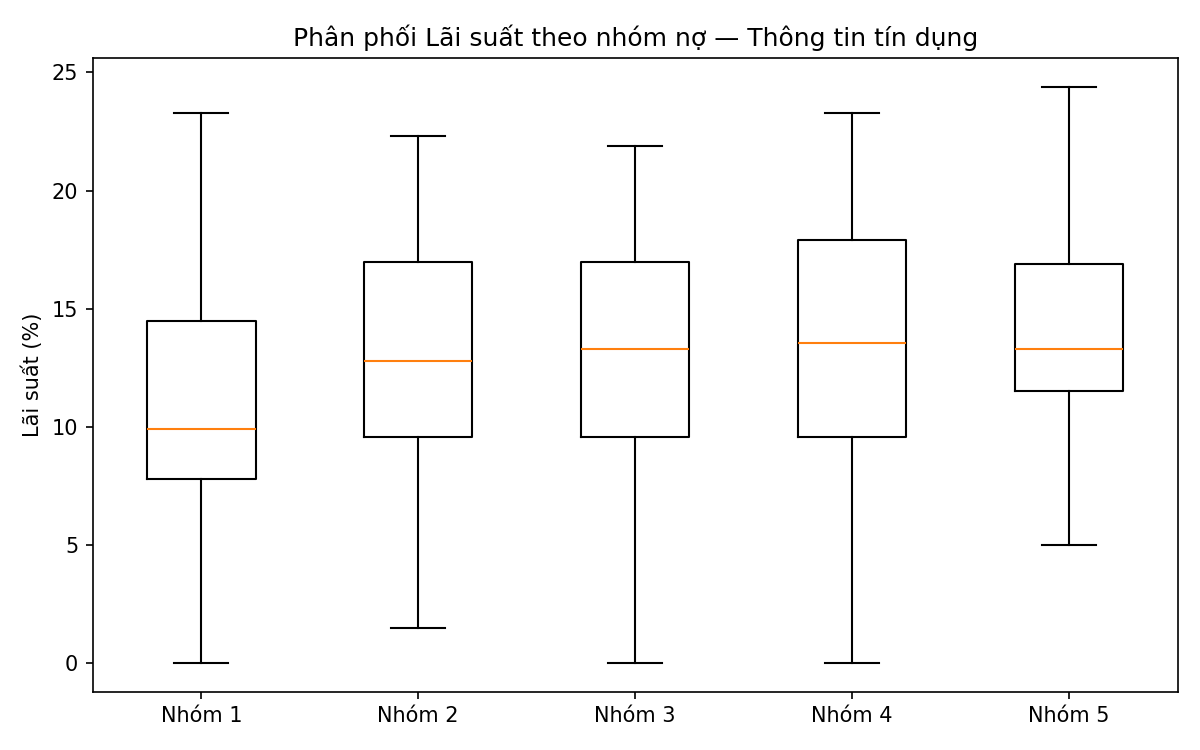
\includegraphics[width=0.7\textwidth]{figures/eda_credit_info_boxplot_laisuat.png}
\caption{Phân phối Lãi suất theo nhóm nợ — bộ dữ liệu B (kỳ 20260430)}
\label{fig:eda-b-box}
\end{figure}

Hình \ref{fig:eda-b-box} cho thấy trung vị lãi suất có xu hướng tăng từ nhóm 1 đến nhóm 5. Phân phối của nhóm 3 và nhóm 4 được ước lượng lần lượt từ 998 và 1.446 quan sát (Bảng \ref{tab:split-distribution}), qua đó hạn chế ảnh hưởng của biến động do cỡ mẫu nhỏ.

\section{Bước 3: Tiền xử lý \& chọn biến}
\label{sec:step3-preprocess}

Bước thứ ba xây dựng tập đặc trưng dùng cho huấn luyện, bao gồm loại các trường có nguy cơ rò rỉ dữ liệu, tạo đặc trưng nghiệp vụ, tính Weight of Evidence và Information Value (WOE/IV), xác lập tập đặc trưng, xử lý giá trị thiếu, mã hóa và chuẩn hóa. Mọi tham số tiền xử lý, như trung vị, trung bình, độ lệch chuẩn và danh mục mã hóa, chỉ được ước lượng trên tập huấn luyện để tránh rò rỉ thông tin từ tập kiểm định.

\subsection{Kiểm soát rò rỉ dữ liệu}
\label{sec:leakage-a}

Rò rỉ thông tin phát sinh khi biến đầu vào chứa dữ liệu chỉ xuất hiện sau thời điểm dự báo hoặc là phép biến đổi trực tiếp của biến đích. Đối với bộ A, các biến \mbox{\texttt{NHOMNO\_TCBS}} và \texttt{NHOMNO} được loại khỏi tập đầu vào; trong đó, \texttt{NHOMNO} có tương quan rất cao với \mbox{\texttt{NHOMNOMOI}}, nên việc giữ lại biến này có thể khiến mô hình tái tạo gần như trực tiếp quy tắc hình thành nhãn. Quá trình sàng lọc cũng loại biến \mbox{\texttt{DUNO\_QD}} bị trùng lặp, trường mô tả văn bản trùng với mã sản phẩm và các trường hằng số hoặc có lượng thông tin không đáng kể.

Ở bộ B, bảy trường bị loại vì có quan hệ trực tiếp với quy tắc phân loại nhóm nợ theo quy định của Ngân hàng Nhà nước: \texttt{Nhóm nợ phân loại sau khi tham chiếu CIC} (một biến thể khác của biến đích); \texttt{Dư nợ gốc chậm trả thực tế}, \texttt{Ngày chậm trả nợ gốc}, \texttt{Số tiền lãi chậm trả thực tế} và \texttt{Ngày chậm trả nợ lãi} (số ngày và số tiền chậm trả là căn cứ trực tiếp để phân loại nhóm nợ); cùng với \texttt{Dự phòng cụ thể phải trích nội bảng} và \texttt{Dự phòng cụ thể đã trích nội bảng}. Tỷ lệ trích lập dự phòng cụ thể là hàm xác định theo nhóm nợ, lần lượt bằng 0\%, 5\%, 20\%, 50\% và 100\% đối với nhóm 1 đến nhóm 5. Việc giữ các trường này có thể làm phát sinh rò rỉ thông tin, khiến mô hình tái tạo quy tắc hình thành nhãn thay vì nhận diện tín hiệu dự báo.

Đối với bài toán dự báo chuyển nhóm nợ, yêu cầu kiểm soát rò rỉ cần được thực hiện chặt chẽ hơn: mọi đặc trưng $X_{i,t}$ phải sẵn có tại hoặc trước thời điểm $t$, trong khi nhãn được xác định trong khoảng từ $t+1$ đến $t+h$. Phép chia mẫu ngẫu nhiên được sử dụng trong nghiên cứu hiện tại phù hợp với mục tiêu kiểm định mô hình phân loại trạng thái, nhưng chưa tối ưu cho bài toán cảnh báo sớm. Khi có dữ liệu theo thời gian, việc chia mẫu theo trình tự thời gian là cần thiết để ngăn thông tin tương lai tham gia quá trình huấn luyện.

\subsection{Xây dựng đặc trưng nghiệp vụ}

Hai nhánh dữ liệu sử dụng công thức tạo biến khác nhau. Bộ A tạo ba biến từ ngày mở, ngày đáo hạn, dư nợ hiện tại và dư nợ gốc. Bộ B tạo bốn biến kỹ thuật từ ngày giải ngân, ngày kết thúc khế ước và số lần cơ cấu lại thời hạn trả nợ.

Các biến này không tồn tại trực tiếp trong dữ liệu ban đầu mà được xây dựng từ một hoặc nhiều trường gốc nhằm chuyển thông tin kỹ thuật thành các đại lượng có ý nghĩa nghiệp vụ rõ ràng hơn. Bảng \ref{tab:engineered-features} tổng hợp nguồn hình thành và cách diễn giải của toàn bộ 7 biến được bổ sung.

{\footnotesize
\begin{longtable}{|p{0.6cm}|p{3.3cm}|p{3.3cm}|p{5.7cm}|}
\caption{Các biến được xây dựng thêm từ dữ liệu ban đầu}
\label{tab:engineered-features}\\
\hline
Bộ & Biến được tạo thêm & Biến gốc sử dụng & Ý nghĩa và cách diễn giải \\
\hline
\endfirsthead
\hline
Bộ & Biến được tạo thêm & Biến gốc sử dụng & Ý nghĩa và cách diễn giải \\
\hline
\endhead
A & \texttt{\seqsplit{LOAN\_TENURE\_DAYS}} & \texttt{\seqsplit{OPEN\_DATE}}, \texttt{\seqsplit{NGAYDENHAN}} & Tổng thời hạn theo hợp đồng, tính bằng số ngày từ ngày mở đến ngày đáo hạn. Giá trị lớn biểu thị khoản vay có kỳ hạn dài hơn. \\
\hline
A & \texttt{\seqsplit{DAYS\_TO\_MATURITY}} & \texttt{\seqsplit{NGAYDENHAN}}, ngày tham chiếu $d_0$ & Số ngày còn lại đến ngày đáo hạn. Giá trị dương biểu thị khoản vay chưa đáo hạn; bằng 0 là đáo hạn tại ngày tham chiếu; giá trị âm biểu thị khoản vay đã qua ngày đáo hạn. \\
\hline
A & \texttt{\seqsplit{UTIL\_RATE}} & \texttt{\seqsplit{CURR\_BAL}}, \texttt{\seqsplit{BASE\_BAL}} & Tỷ lệ giữa dư nợ hiện tại và dư nợ gốc. Giá trị gần 1 cho biết dư nợ hiện tại xấp xỉ dư nợ gốc; nhỏ hơn 1 phản ánh dư nợ đã giảm; lớn hơn 1 có thể phản ánh giải ngân bổ sung hoặc biến động số dư. \\
\hline
B & \texttt{\seqsplit{ENG\_LOAN\_AGE\_DAYS}} & \texttt{\seqsplit{ETL\_DATE}}, \texttt{Ngày giải ngân} & Số ngày đã trôi qua kể từ ngày giải ngân tới ngày chốt dữ liệu (\texttt{\seqsplit{ETL\_DATE}}) của chính hồ sơ đó, tức tuổi của khoản vay. Giá trị lớn biểu thị khoản vay đã tồn tại lâu hơn. \\
\hline
B & \texttt{\seqsplit{ENG\_DAYS\_TO\_MATURITY}} & \texttt{Ngày kết thúc khế ước}, \texttt{\seqsplit{ETL\_DATE}} & Số ngày còn lại đến ngày kết thúc khế ước, tính từ \texttt{\seqsplit{ETL\_DATE}}. Giá trị âm cho biết khế ước đã qua ngày kết thúc so với ngày chốt dữ liệu. \\
\hline
B & \texttt{\seqsplit{ENG\_TENOR\_ACTUAL\_DAYS}} & \texttt{Ngày kết thúc khế ước}, \texttt{Ngày giải ngân} & Kỳ hạn thực tế của khế ước, bằng chênh lệch giữa ngày kết thúc và ngày giải ngân. \\
\hline
B & \texttt{\seqsplit{ENG\_HAS\_RESTRUCTURE}} & \texttt{Số lần cơ cấu lại thời hạn trả nợ} & Biến nhị phân nhận giá trị 1 khi số lần cơ cấu lại thời hạn trả nợ lớn hơn 0 và nhận giá trị 0 trong trường hợp còn lại (kể cả khi thiếu dữ liệu). Biến chỉ phản ánh việc từng phát sinh cơ cấu, không cho biết mức độ. \\
\hline
\end{longtable}
}

Các biến phát sinh trên được tính hoàn toàn từ các trường đầu vào và không sử dụng biến đích. Do đó, bản thân quá trình tạo biến không trực tiếp làm lộ nhãn nhóm nợ. Tuy nhiên, trước khi triển khai thực tế, thời điểm hình thành của từng trường gốc vẫn phải được kiểm tra để bảo đảm trường đó đã tồn tại tại thời điểm dự báo; nếu một trường chỉ phát sinh sau thời điểm quan sát, biến được tạo từ trường đó vẫn có thể gây rò rỉ thông tin theo thời gian.

\subsubsection{Đặc trưng của bộ dữ liệu A}
\label{sec:feature-a}

Với ngày tham chiếu cố định $d_0=$ 31/12/2021, các biến được tính như sau:
\[
\begin{aligned}
\mathit{LOAN\_TENURE\_DAYS}_i
&=\max\{0,d_i^{\mathrm{maturity}}-d_i^{\mathrm{open}}\},\\
\mathit{DAYS\_TO\_MATURITY}_i
&=d_i^{\mathrm{maturity}}-d_0.
\end{aligned}
\]
Trong đó $d_i^{\mathrm{open}}$ là ngày mở khoản vay; $d_i^{\mathrm{maturity}}$ là ngày đến hạn; chênh lệch ngày được biểu diễn bằng số ngày dương hoặc âm. Việc cố định $d_0$ giúp cùng một hồ sơ nhận cùng giá trị khi tái chạy.

Tỷ lệ sử dụng dư nợ của bộ A được cài đặt:
\[
\mathit{UTIL\_RATE}_i
=
\begin{cases}
\operatorname{clip}\!\left(
\dfrac{\mathit{CURR\_BAL}_i}{\mathit{BASE\_BAL}_i},0,10
\right),&\mathit{BASE\_BAL}_i>0,\\
0,&\mathit{BASE\_BAL}_i\leq0.
\end{cases}
\]
Trong đó \mbox{\texttt{CURR\_BAL}} là dư nợ hiện tại; \mbox{\texttt{BASE\_BAL}} là dư nợ gốc hoặc cơ sở; và toán tử $\operatorname{clip}(x,0,10)$ giới hạn giá trị trong đoạn $[0,10]$ để giảm ảnh hưởng của tỷ số ngoại lệ.

\subsubsection{Kiểm tra đặc trưng đã tạo của bộ dữ liệu A}
\label{sec:feature-a-eda}

Sau khi ba biến \mbox{\texttt{LOAN\_TENURE\_DAYS}}, \mbox{\texttt{DAYS\_TO\_MATURITY}} và \mbox{\texttt{UTIL\_RATE}} được tạo, mục này khảo sát thống kê mô tả, ngoại lệ và tương quan của chúng cùng năm biến gốc đã trình bày ở Bước 2 (mục \ref{sec:eda}), trước khi tính Information Value ở mục sau.

\begin{table}[H]
\centering
\caption{Thống kê mô tả ba biến kỹ thuật của bộ dữ liệu A}
\label{tab:eda-a-describe-eng}
\begin{tabular}{|l|r|r|r|r|r|}
\hline
Biến & Trung bình & Độ lệch chuẩn & Nhỏ nhất & Trung vị & Lớn nhất\\
\hline
\texttt{\seqsplit{LOAN\_TENURE\_DAYS}} & 2.292,5 & 2.452,0 & 0 & 1.461 & 18.292\\
\texttt{\seqsplit{DAYS\_TO\_MATURITY}} & 672,7 & 2.397,7 & $-5.513$ & 96 & 16.798\\
\texttt{\seqsplit{UTIL\_RATE}} & 2,4561 & 3,2557 & $2\times10^{-8}$ & 0,9429 & 10,0000\\
\hline
\end{tabular}
\end{table}

\begin{table}[H]
\centering
\caption{Số quan sát ngoại lệ theo IQR — ba biến kỹ thuật của bộ dữ liệu A}
\label{tab:eda-a-outlier-eng}
\begin{tabular}{|l|r|r|}
\hline
Biến & Số ngoại lệ & Tỷ lệ (\%)\\
\hline
\texttt{\seqsplit{DAYS\_TO\_MATURITY}} & 6.233 & 23,08\\
\texttt{\seqsplit{UTIL\_RATE}} & 4.646 & 17,21\\
\texttt{\seqsplit{LOAN\_TENURE\_DAYS}} & 2.754 & 10,20\\
\hline
\end{tabular}
\end{table}

\mbox{\texttt{DAYS\_TO\_MATURITY}} có tỷ lệ ngoại lệ cao nhất (23,08\%) vì biến này nhận cả giá trị âm (khoản vay đã quá hạn đáo hạn tính đến ngày tham chiếu $d_0$) lẫn giá trị dương lớn (khoản vay kỳ hạn dài); đây là đặc điểm nghiệp vụ thực, không phải lỗi dữ liệu, nên không bị loại hay cắt ngưỡng. Ngược lại, \mbox{\texttt{UTIL\_RATE}} có 17,21\% ngoại lệ chủ yếu do một bộ phận khách hàng có dư nợ hiện tại vượt xa dư nợ gốc ban đầu (ví dụ giải ngân bổ sung nhiều lần); đây chính là lý do công thức tính \mbox{\texttt{UTIL\_RATE}} ở trên chủ động \textbf{clip} kết quả vào đoạn $[0,10]$: nếu không giới hạn, một số ít hồ sơ có tỷ lệ hàng trăm lần sẽ làm lệch cực đoan bước chuẩn hóa z-score của \emph{toàn bộ} biến này khi đưa vào Logistic Regression.

Trong nghiên cứu này, \textbf{clip dữ liệu} được hiểu là phép giới hạn giá trị của một biến trong một khoảng xác định, thay vì loại bỏ các quan sát nằm ngoài khoảng đó. Với $u$ là giá trị ban đầu của \mbox{\texttt{UTIL\_RATE}}, giá trị sau khi giới hạn được xác định như sau:
\[
\operatorname{clip}(u;0,10)=\min\{\max(u,0),10\}.
\]
Theo đó, giá trị nhỏ hơn 0 được thay bằng 0, giá trị lớn hơn 10 được thay bằng 10, còn các giá trị thuộc đoạn $[0,10]$ được giữ nguyên. Ngưỡng trên bằng 10 tương ứng với trường hợp dư nợ hiện tại bằng 10 lần dư nợ gốc. Cách xử lý này không làm giảm số lượng quan sát và vẫn bảo lưu thông tin rằng hồ sơ có mức sử dụng rất cao, đồng thời hạn chế ảnh hưởng chi phối của một số giá trị cực đoan đối với trung bình, độ lệch chuẩn và quá trình ước lượng mô hình. Tuy nhiên, sau khi giới hạn, các mức \mbox{\texttt{UTIL\_RATE}} lớn hơn 10 không còn được phân biệt với nhau; vì vậy, đây là một lựa chọn tiền xử lý nhằm tăng tính ổn định của mô hình, không hàm ý rằng các giá trị vượt ngưỡng là sai về mặt nghiệp vụ.

\begin{figure}[H]
\centering
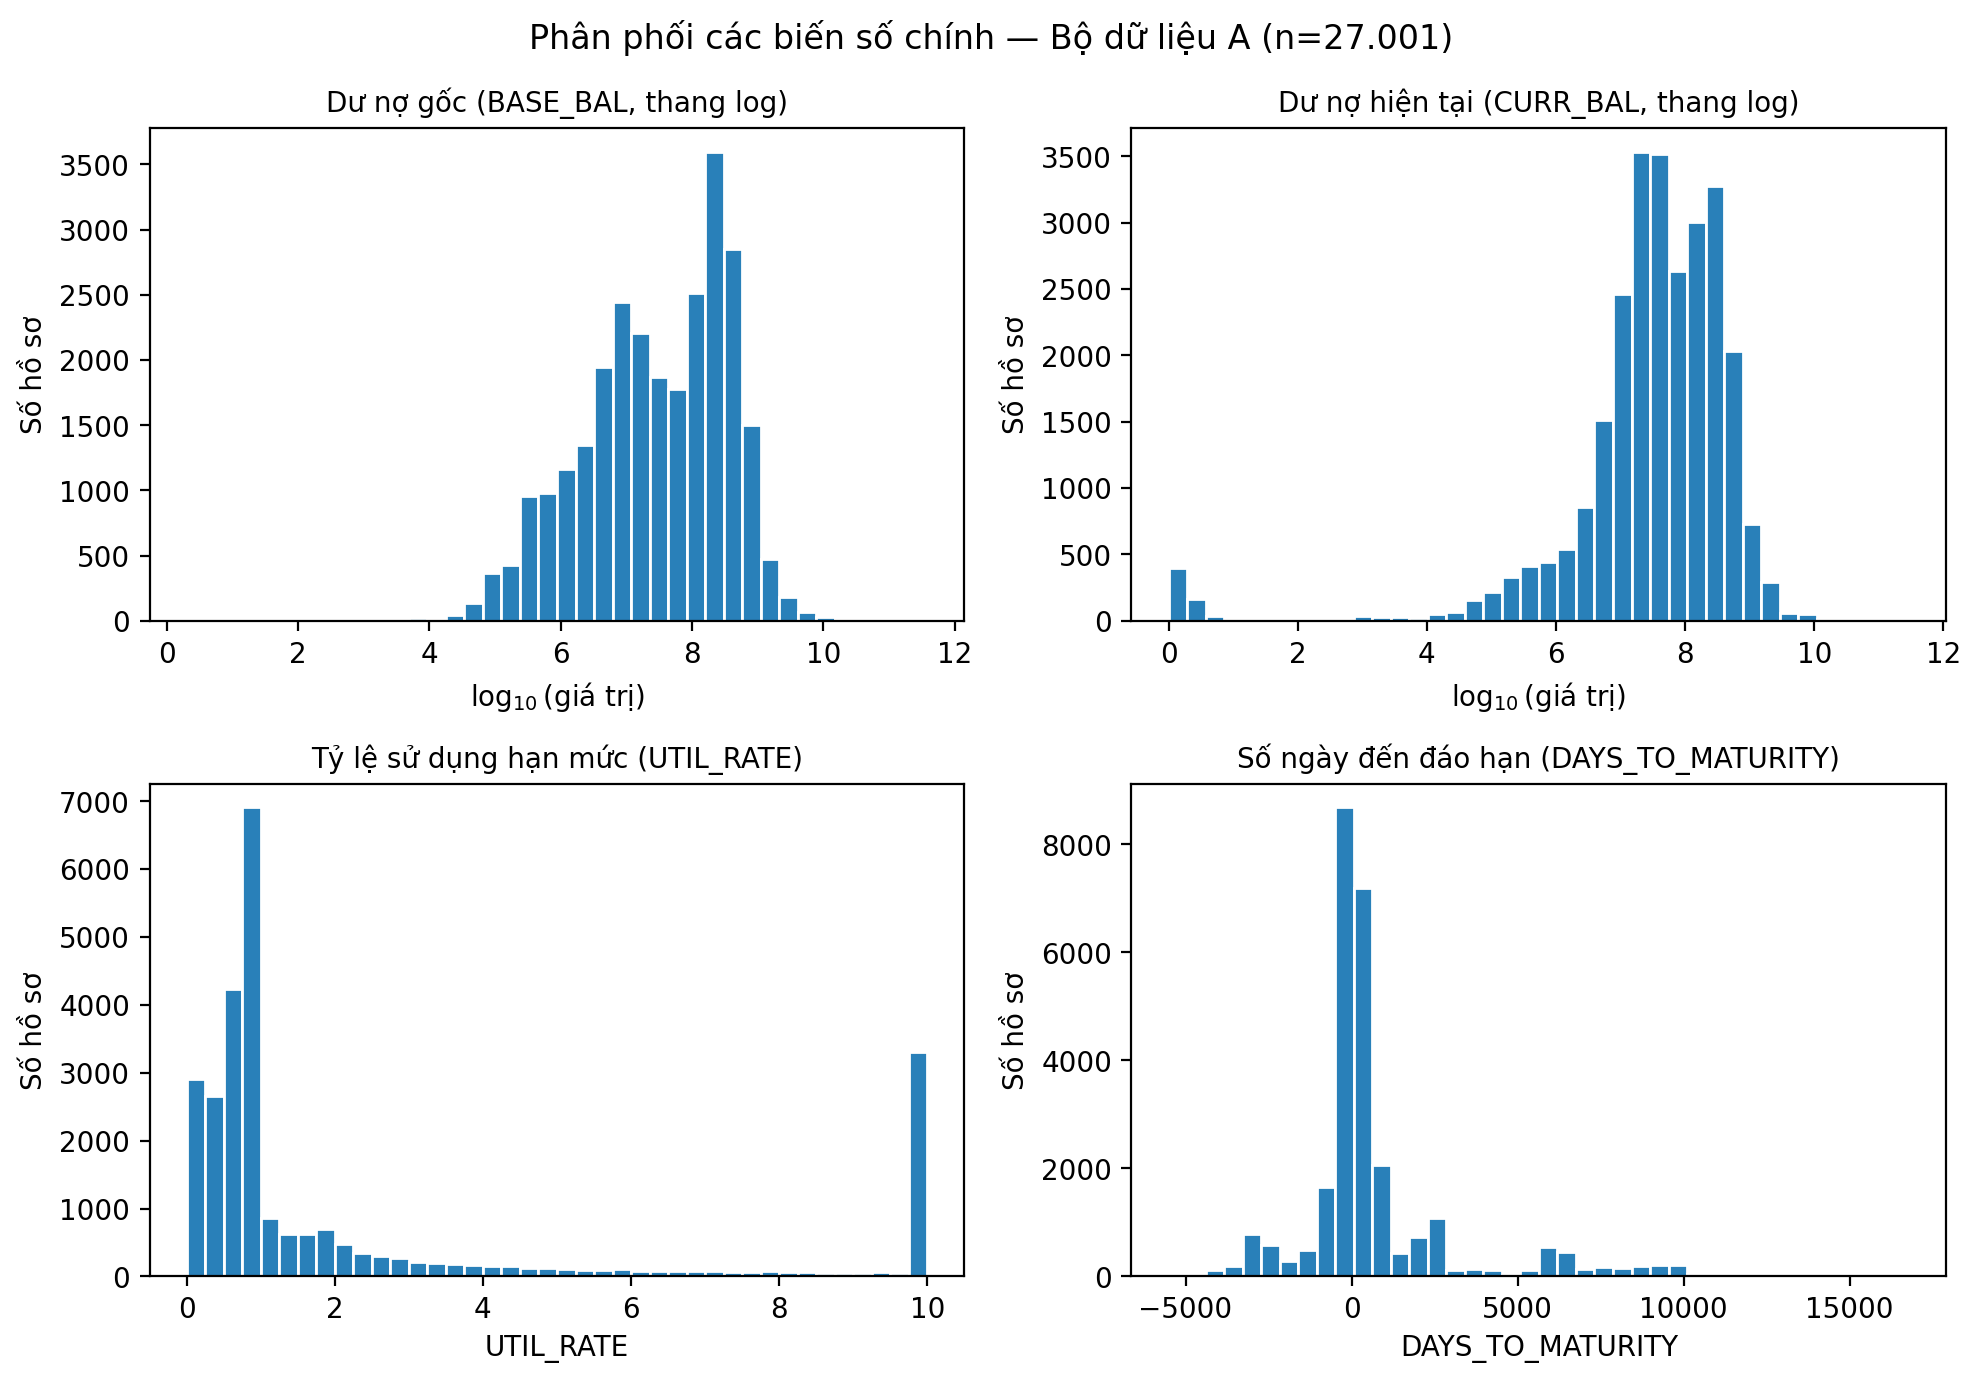
\includegraphics[width=0.95\textwidth]{figures/eda_a_histograms.png}
\caption{Phân phối bốn biến số chính của bộ dữ liệu A (n=27.001)}
\label{fig:eda-a-hist}
\end{figure}

Hình \ref{fig:eda-a-hist} minh họa trực quan hai đặc điểm đã nêu bằng số: \mbox{\texttt{BASE\_BAL}} và \mbox{\texttt{CURR\_BAL}} lệch phải mạnh trên thang gốc nên được vẽ theo $\log_{10}$ để thấy rõ hình chuông tương đối; \mbox{\texttt{UTIL\_RATE}} có một cột dồn rõ rệt tại đúng giá trị 10, bằng chứng trực quan cho thấy phép \textbf{clip} đã cắt và dồn một lượng đáng kể hồ sơ (khoảng 3.200, tương ứng phần vượt ngưỡng của 17,21\% ngoại lệ ở Bảng \ref{tab:eda-a-outlier-eng}) về đúng biên trên; \mbox{\texttt{DAYS\_TO\_MATURITY}} có hai đỉnh, một quanh 0 (khoản vay gần đáo hạn hoặc mới quá hạn) và một dải trải dài về phía dương (khoản vay kỳ hạn dài).

Ma trận tương quan (Bảng \ref{tab:eda-a-corr}, minh họa trực quan ở Hình \ref{fig:eda-a-corr}) cho thấy ba cặp biến có $|r|\geq 0,7$.

\begin{table}[H]
\centering
\caption{Các cặp biến số tương quan mạnh nhất — bộ dữ liệu A}
\label{tab:eda-a-corr}
\begin{tabular}{|l|l|r|}
\hline
Biến 1 & Biến 2 & Hệ số tương quan $r$\\
\hline
\texttt{\seqsplit{LOAN\_TENURE\_DAYS}} & \texttt{\seqsplit{DAYS\_TO\_MATURITY}} & 0,942\\
\texttt{\seqsplit{BASE\_BAL}} & \texttt{\seqsplit{CURR\_BAL}} & 0,923\\
\texttt{ORGNBR} & \texttt{\seqsplit{PARENTORGNBR}} & 0,738\\
\texttt{LAISUAT} & \texttt{\seqsplit{LOAN\_TENURE\_DAYS}} & 0,352\\
\texttt{LAISUAT} & \texttt{\seqsplit{UTIL\_RATE}} & $-0,327$\\
\hline
\end{tabular}
\end{table}

Ba cặp tương quan mạnh nhất đều có cách giải thích nghiệp vụ trực tiếp: \mbox{\texttt{LOAN\_TENURE\_DAYS}} và \mbox{\texttt{DAYS\_TO\_MATURITY}} cùng được tính từ ngày mở và ngày đáo hạn nên gần như là hai phép biến đổi tuyến tính của cùng thông tin gốc; \mbox{\texttt{CURR\_BAL}} là dư nợ hiện tại nên tương quan cao với dư nợ gốc \mbox{\texttt{BASE\_BAL}}; \texttt{ORGNBR} và \mbox{\texttt{PARENTORGNBR}} phản ánh cấu trúc phân cấp chi nhánh--đơn vị cấp trên. Mức tương quan này không đủ cao để loại biến (không có cặp nào $|r|>0,95$), nhưng đủ để giải thích vì sao trong bảng SHAP ở Chương 4, importance của hai biến kỳ hạn thường lấn át lẫn nhau tùy ngẫu nhiên hoá của mô hình cây; đây là hạn chế cố hữu khi diễn giải importance trên các biến tương quan \cite{lundberg2017unified}.

\begin{figure}[H]
\centering
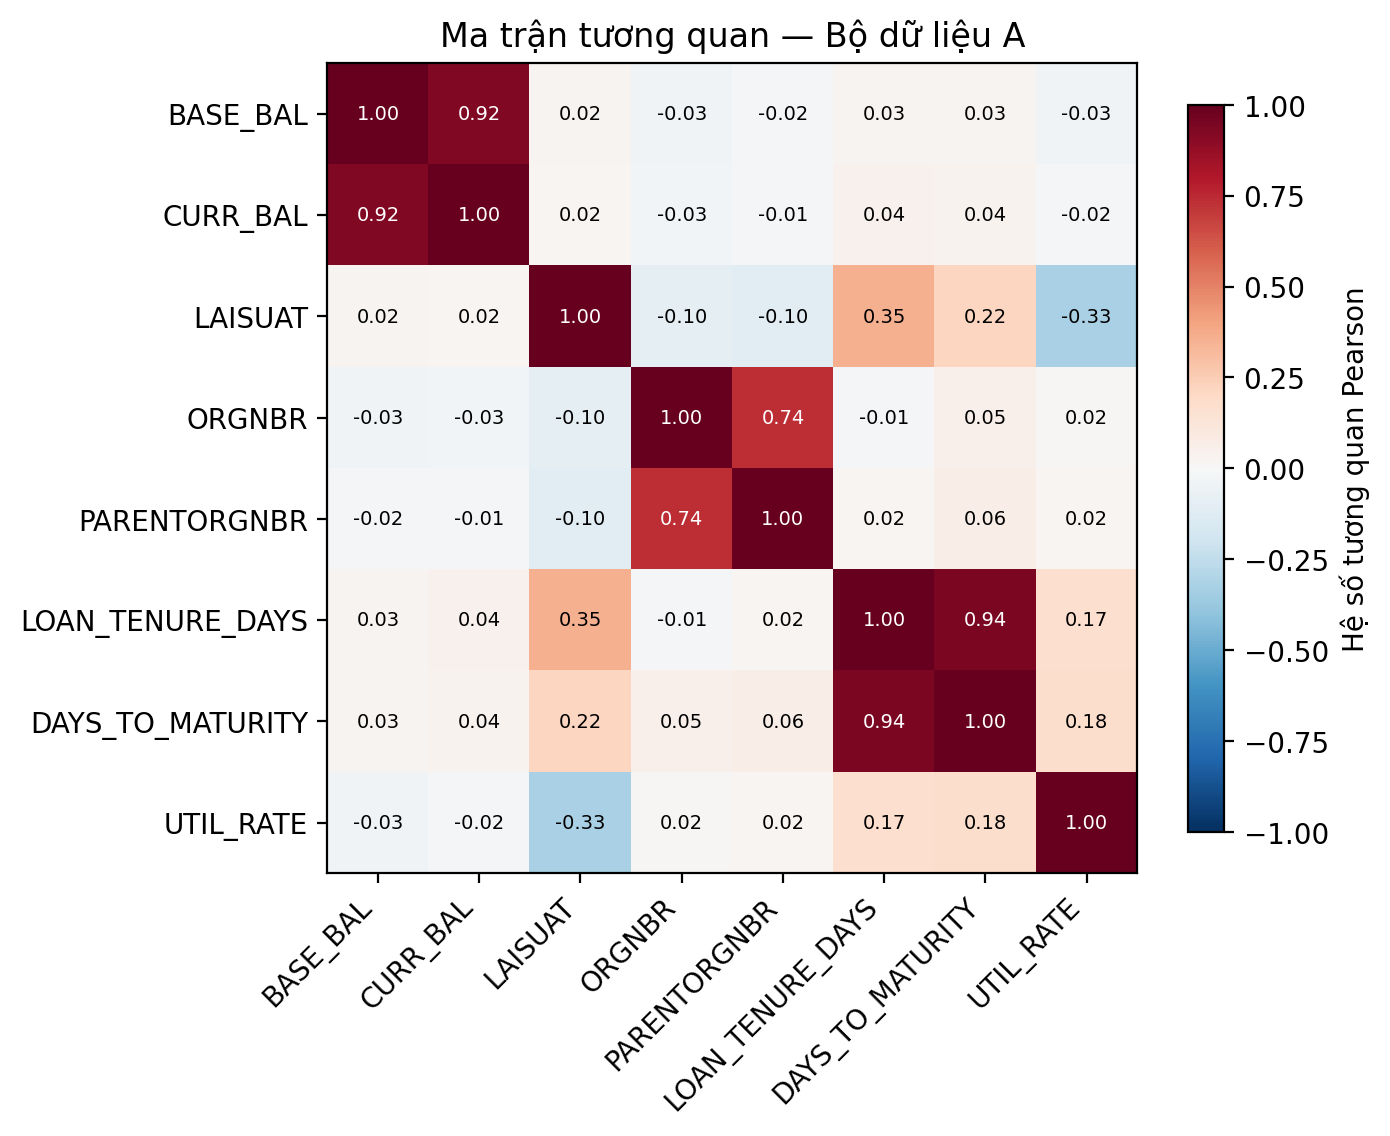
\includegraphics[width=0.75\textwidth]{figures/eda_a_correlation.png}
\caption{Ma trận tương quan Pearson giữa các biến số của bộ dữ liệu A}
\label{fig:eda-a-corr}
\end{figure}

\begin{figure}[H]
\centering
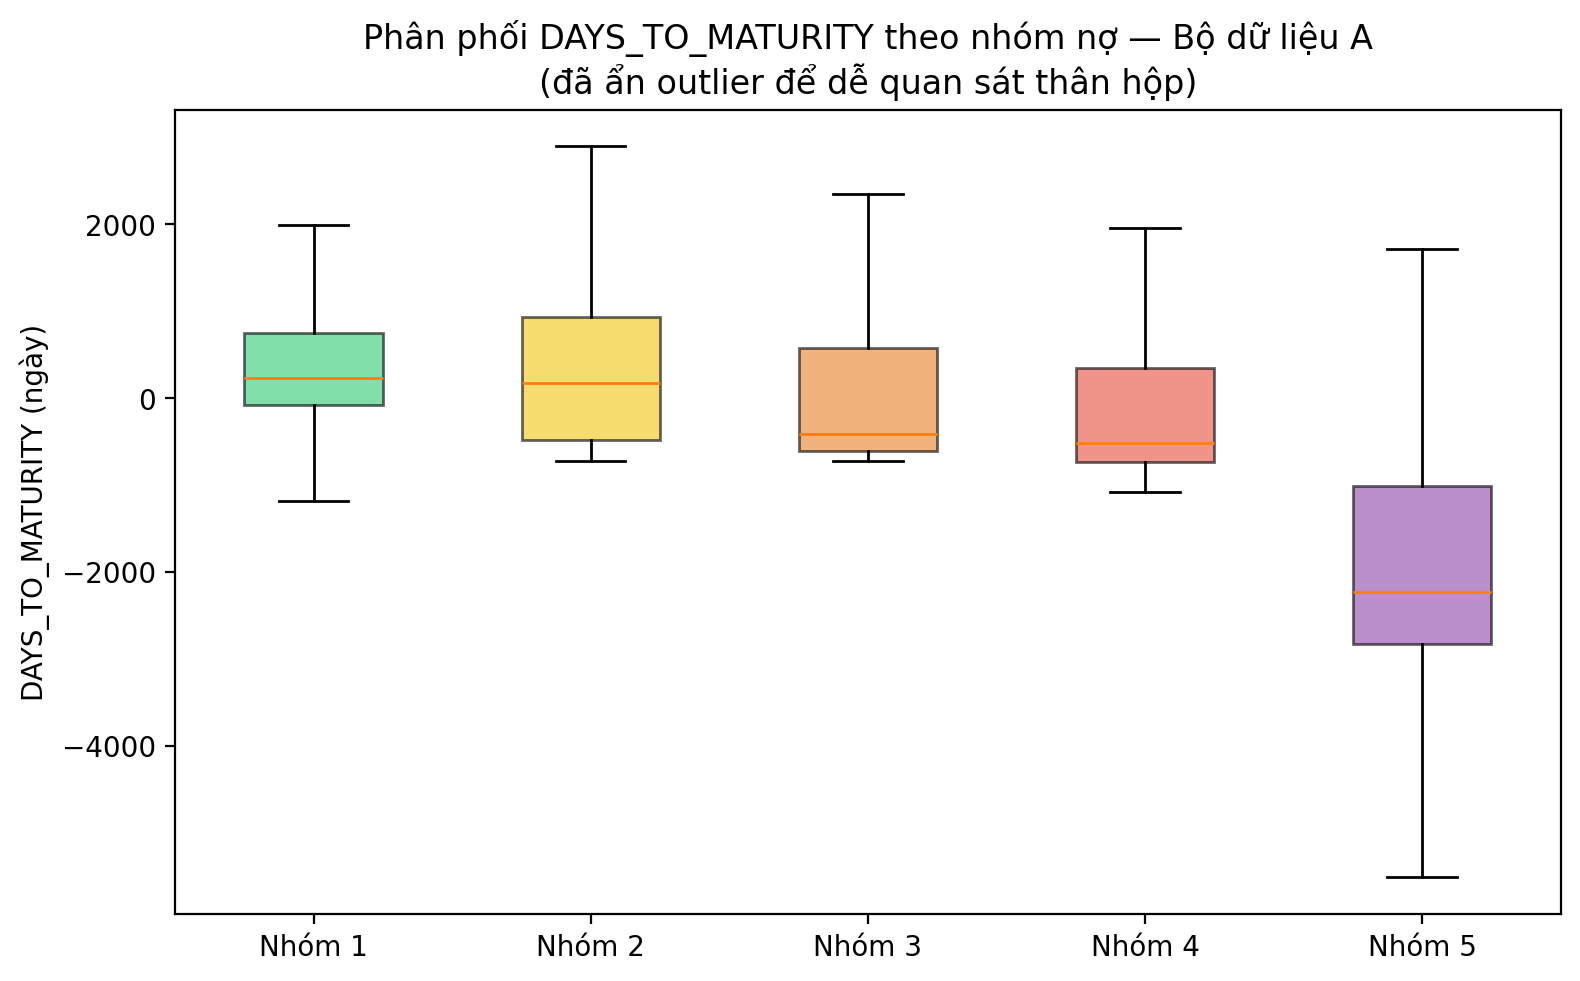
\includegraphics[width=0.7\textwidth]{figures/eda_a_boxplot_daystomaturity.png}
\caption{Phân phối \mbox{\texttt{DAYS\_TO\_MATURITY}} theo nhóm nợ — bộ dữ liệu A}
\label{fig:eda-a-box}
\end{figure}

Hình \ref{fig:eda-a-box} cho thấy trung vị \mbox{\texttt{DAYS\_TO\_MATURITY}} giảm dần khá đều từ nhóm 1 đến nhóm 4 rồi đổi hướng ở nhóm 5, phù hợp việc đây là biến SHAP xếp hạng cao nhất ở Chương 4, nhưng cũng gợi ý quan hệ giữa biến này và nhóm nợ không hoàn toàn đơn điệu, cần thận trọng khi diễn giải nhân quả.

\subsubsection{Đặc trưng thời gian của bộ dữ liệu B}
\label{sec:eng-util-b}

Ba trong bốn biến kỹ thuật của bộ B được tính bằng chênh lệch ngày, sử dụng \mbox{\texttt{ETL\_DATE}} của từng hồ sơ làm mốc tham chiếu để bảo đảm khả năng tái lập kết quả. Mỗi hồ sơ có một ngày chốt dữ liệu cố định tại thời điểm trích xuất báo cáo, nên giá trị của các biến thời gian không thay đổi khi thực thi lại mã nguồn tại một thời điểm khác. Biến còn lại được tính trực tiếp từ số lần cơ cấu lại thời hạn trả nợ.

\[
\begin{aligned}
\mathit{ENG\_LOAN\_AGE\_DAYS}_i
&= \mathit{ETL\_DATE}_i - d_i^{\mathrm{disb}},\\
\mathit{ENG\_DAYS\_TO\_MATURITY}_i
&= d_i^{\mathrm{end}} - \mathit{ETL\_DATE}_i,\\
\mathit{ENG\_TENOR\_ACTUAL\_DAYS}_i
&= d_i^{\mathrm{end}} - d_i^{\mathrm{disb}},
\end{aligned}
\]
trong đó $d_i^{\mathrm{disb}}$ là ngày giải ngân; $d_i^{\mathrm{end}}$ là ngày kết thúc khế ước; và $\mathit{ETL\_DATE}_i$ là ngày chốt dữ liệu của hồ sơ $i$. Biến nhị phân còn lại:
\[
\mathit{ENG\_HAS\_RESTRUCTURE}_i
=
\begin{cases}
1, & \mathit{SoLanCoCauLai}_i>0,\\
0, & \text{ngược lại (kể cả khi thiếu dữ liệu)}.
\end{cases}
\]

Trường \texttt{Thời điểm truy đòi}, ban đầu được xem xét làm nguồn cho một biến thời gian thứ năm, bị loại khỏi danh sách cột ngày sau khi kiểm tra thực nghiệm cho thấy trường này trùng khớp 100\% với \texttt{Ngày kết thúc khế ước} trên toàn bộ dữ liệu quan sát được; giữ lại sẽ chỉ tạo ra một biến kỹ thuật trùng lặp hoàn toàn với \mbox{\texttt{ENG\_DAYS\_TO\_MATURITY}}, không bổ sung thông tin mới.

\subsubsection{Kiểm tra đặc trưng đã tạo của bộ dữ liệu B}
\label{sec:feature-b-eda}

Cả bốn biến kỹ thuật của bộ B đều \textbf{không có giá trị thiếu} (0,00\%), vì được tính trực tiếp từ \mbox{\texttt{ETL\_DATE}}, ngày giải ngân và ngày kết thúc khế ước, ba trường có mặt ở toàn bộ 100.617 hồ sơ. Bảng \ref{tab:eda-b-describe-eng} trình bày thống kê mô tả.

\begin{table}[H]
\centering
\caption{Thống kê mô tả bốn biến kỹ thuật của bộ dữ liệu B}
\label{tab:eda-b-describe-eng}
\begin{tabular}{|l|r|r|r|r|}
\hline
Biến & Trung bình & Độ lệch chuẩn & Trung vị & Ngoại lệ IQR (\%)\\
\hline
\texttt{\seqsplit{ENG\_LOAN\_AGE\_DAYS}} & 602,82 & 632,71 & 395 & 3,05\\
\texttt{\seqsplit{ENG\_DAYS\_TO\_MATURITY}} & 1.667,40 & 2.778,31 & 711 & 11,51\\
\texttt{\seqsplit{ENG\_TENOR\_ACTUAL\_DAYS}} & 2.270,22 & 2.850,29 & 1.461 & 12,45\\
\texttt{\seqsplit{ENG\_HAS\_RESTRUCTURE}} & 0,004 & 0,063 & 0 & 0,40\\
\hline
\end{tabular}
\end{table}

\begin{figure}[H]
\centering
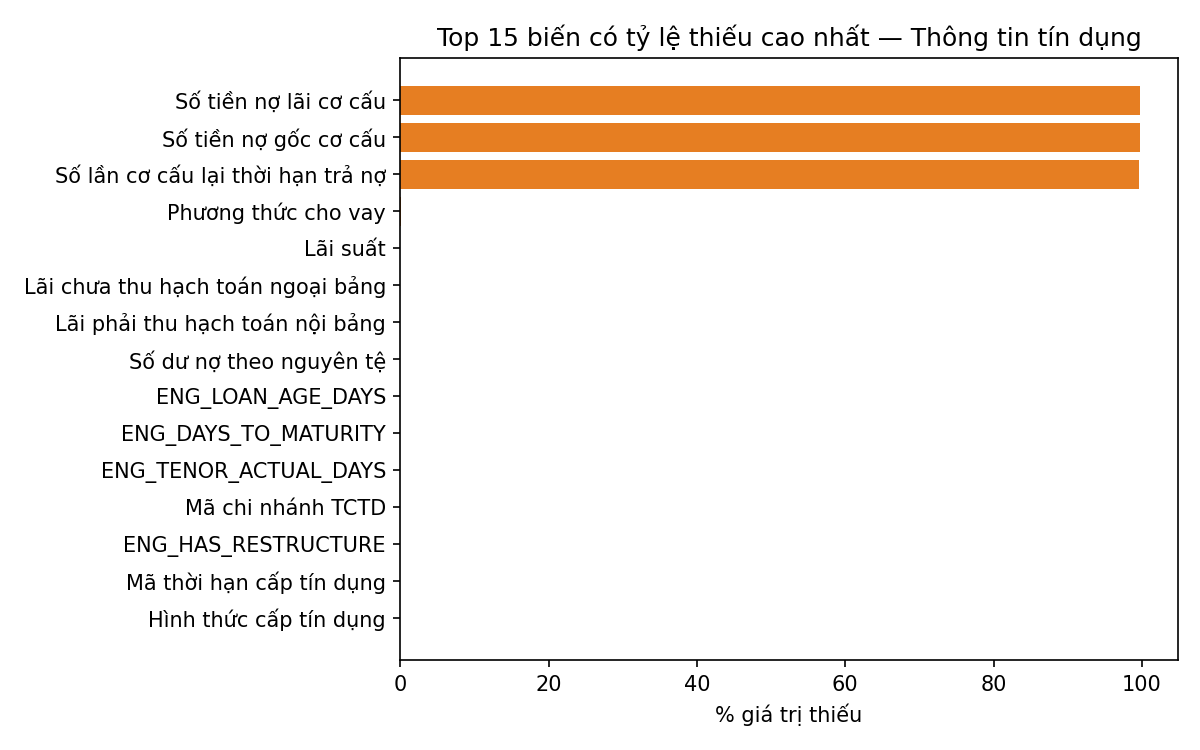
\includegraphics[width=0.85\textwidth]{figures/eda_credit_info_missing.png}
\caption{Top 15 biến (trong bể đặc trưng hợp lệ) có tỷ lệ thiếu cao nhất — bộ dữ liệu B}
\label{fig:eda-b-missing}
\end{figure}

\begin{figure}[H]
\centering
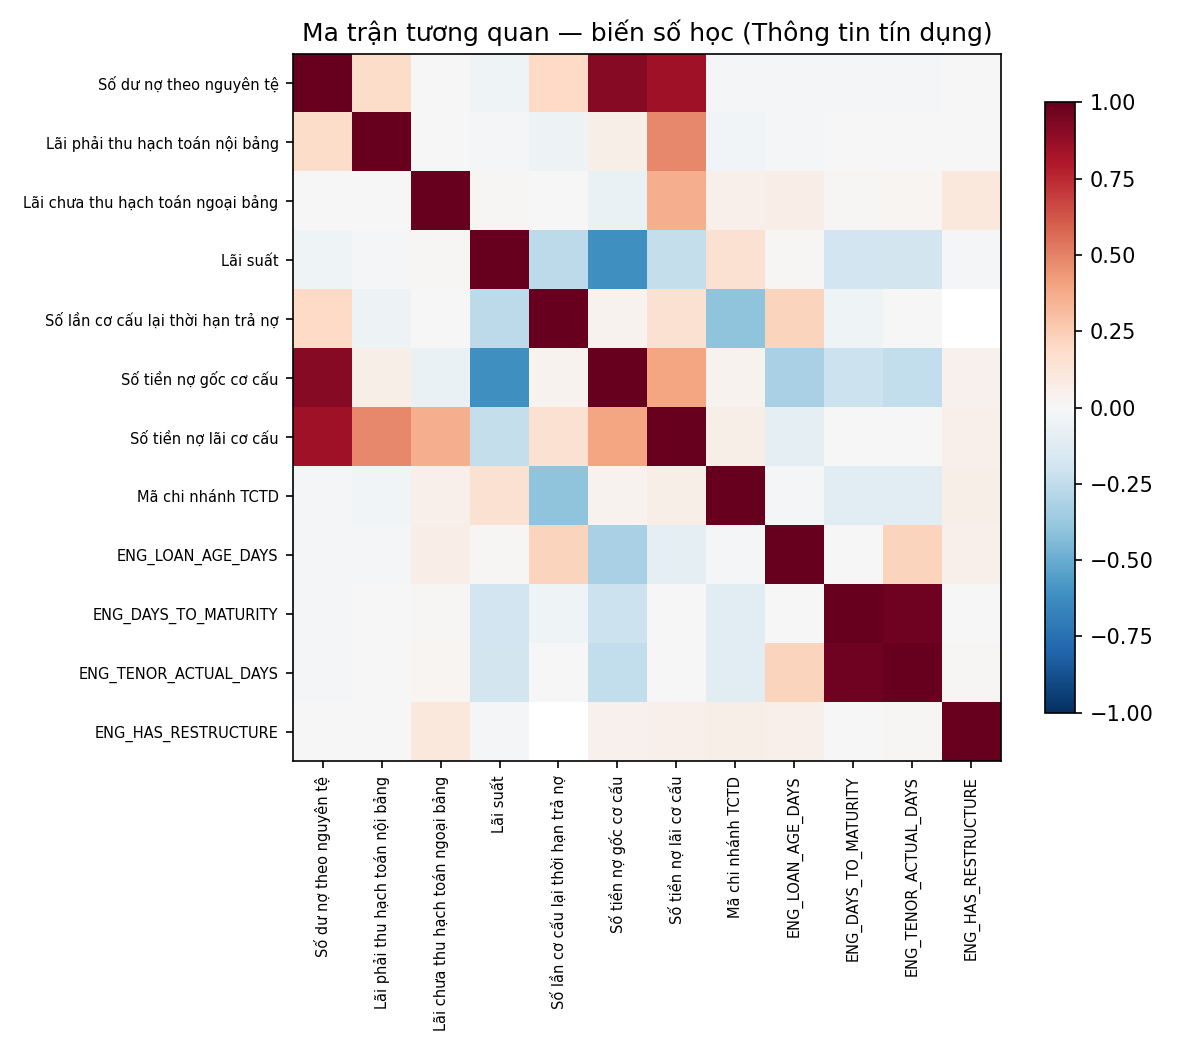
\includegraphics[width=0.8\textwidth]{figures/eda_credit_info_correlation.png}
\caption{Ma trận tương quan giữa 12 biến số (8 biến gốc + 4 biến kỹ thuật) — bộ dữ liệu B}
\label{fig:eda-b-corr}
\end{figure}

Hình \ref{fig:eda-b-corr} cho thấy cặp \mbox{\texttt{ENG\_DAYS\_TO\_MATURITY}} và \mbox{\texttt{ENG\_TENOR\_ACTUAL\_DAYS}} có hệ số tương quan lớn nhất trong 12 biến số ($r=0,975$). Mối tương quan này xuất phát từ việc cả hai đặc trưng cùng sử dụng mốc \texttt{Ngày kết thúc khế ước}, tương tự mối quan hệ giữa \mbox{\texttt{LOAN\_TENURE\_DAYS}} và \mbox{\texttt{DAYS\_TO\_MATURITY}} ở bộ A (Mục \ref{sec:feature-a-eda}). Do hệ số tương quan vượt ngưỡng tham khảo 0,95, hai biến có khả năng chứa thông tin trùng lặp đáng kể. Tuy vậy, nghiên cứu vẫn giữ lại cả hai do chúng biểu thị hai khía cạnh nghiệp vụ khác nhau, lần lượt là kỳ hạn còn lại và tổng kỳ hạn thực tế. Đây là điểm cần thận trọng khi diễn giải mức độ quan trọng ở Chương 4, bởi đóng góp của hai biến có thể cùng bắt nguồn từ một nguồn thông tin cơ sở.

\subsection{Weight of Evidence và Information Value (WOE/IV)}

Information Value (IV) được sử dụng để lượng hóa khả năng phân tách giữa nhóm nợ ``tốt'' và nhóm nợ ``xấu'' của từng biến trước khi đưa vào mô hình. Nghiên cứu quy ước nhãn nhị phân ``tốt'' tương ứng với nhóm 1 và ``xấu'' tương ứng với các nhóm 2--5; các biến số được chia thành 10 khoảng theo phân vị. IV được tính trên tập đặc trưng còn lại sau khi loại các trường có nguy cơ rò rỉ tại Mục \ref{sec:leakage-a} và bổ sung các đặc trưng nghiệp vụ, qua đó cung cấp căn cứ định lượng để xác lập tập đặc trưng tại Mục \ref{sec:pool-a}.

\subsubsection{Bảng Information Value đầy đủ của bộ dữ liệu A}
\label{sec:iv-a}

Bảng \ref{tab:iv-a} trình bày giá trị IV của toàn bộ 13 biến trong tập phân tích, bao gồm \texttt{SEX} và \texttt{LOAIKH}, theo thứ tự giảm dần. Vai trò của hai biến này trong quá trình lựa chọn tập đặc trưng được thảo luận tại Mục \ref{sec:pool-a}.

\begin{table}[H]
\centering
\caption{Information Value của 13 biến — bộ dữ liệu A}
\label{tab:iv-a}
\begin{tabular}{|l|r|l|}
\hline
Biến & IV & Mức\\
\hline
\texttt{\seqsplit{DAYS\_TO\_MATURITY}} & 4,5541 & (!) Nghi ngờ (leakage?)\\
\texttt{\seqsplit{CURRMIACCTTYPCD}} & 1,9921 & (!) Nghi ngờ (leakage?)\\
\texttt{\seqsplit{LOAN\_TENURE\_DAYS}} & 1,9410 & (!) Nghi ngờ (leakage?)\\
\texttt{\seqsplit{MUCDICHVAY}} & 1,4141 & (!) Nghi ngờ (leakage?)\\
\texttt{\seqsplit{UTIL\_RATE}} & 1,3334 & (!) Nghi ngờ (leakage?)\\
\texttt{\seqsplit{MJACCTTYPCD}} & 0,9695 & Rất mạnh\\
\texttt{LAISUAT} & 0,7851 & Rất mạnh\\
\texttt{\seqsplit{BASE\_BAL}} & 0,5356 & Rất mạnh\\
\texttt{\seqsplit{PARENTORGNBR}} & 0,3201 & Mạnh\\
\texttt{\seqsplit{CURR\_BAL}} & 0,2585 & Trung bình\\
\texttt{ORGNBR} & 0,1820 & Trung bình\\
\texttt{SEX} & 0,0081 & Vô dụng\\
\texttt{LOAIKH} & 0,0000 & Vô dụng\\
\hline
\end{tabular}
\end{table}

Kết quả cho thấy 5 trong tổng số 13 biến có $IV>1{,}0$, vượt ngưỡng mà Siddiqi xem là dấu hiệu cần thận trọng do biến có thể đại diện gián tiếp hoặc làm rò rỉ biến đích \cite{siddiqi2006credit}. Năm biến này đồng thời nằm trong nhóm có mức độ quan trọng cao nhất theo SHAP và Gain ở Chương 4. Có hai khả năng cần được phân biệt. Thứ nhất, nếu biến được tính trực tiếp từ \mbox{\texttt{NHOMNOMOI}} hoặc từ quy tắc hình thành nhãn, biến đó phải được loại tương tự \mbox{\texttt{NHOMNO}} tại Mục \ref{sec:leakage-a}. Thứ hai, nếu biến được xác lập độc lập với nhãn nhưng có quan hệ nghiệp vụ chặt chẽ với nhóm nợ, IV cao có thể phản ánh tín hiệu thực tế. Do chưa có đầy đủ thông tin về quy trình hình thành dữ liệu nguồn, kết quả này được xem là một giới hạn cần lưu ý khi diễn giải mô hình.

Luận văn nghiêng về khả năng thứ hai đối với ba biến được xây dựng trong nghiên cứu. Cụ thể, \mbox{\texttt{DAYS\_TO\_MATURITY}} phản ánh số ngày còn lại đến ngày đáo hạn; \mbox{\texttt{LOAN\_TENURE\_DAYS}} biểu thị thời hạn khoản vay; và \mbox{\texttt{UTIL\_RATE}} đo lường tỷ lệ sử dụng dư nợ. Cả ba biến đều được tính từ ngày mở khoản vay, ngày đáo hạn hoặc số dư nợ. Các trường dữ liệu nguồn này tồn tại độc lập với quy trình xếp nhóm nợ và không phải là biến phái sinh của \mbox{\texttt{NHOMNOMOI}}. Tuy nhiên, với hai biến phân loại nhiều danh mục \mbox{\texttt{CURRMIACCTTYPCD}} (31 nhóm) và \mbox{\texttt{MUCDICHVAY}} (79 nhóm), IV cao một phần có thể là hiện tượng thống kê: biến định danh có rất nhiều danh mục dễ đạt IV cao giả tạo vì mỗi danh mục nhỏ đóng góp lệch xác suất riêng, ngay cả khi không có quan hệ nhân quả mạnh; đây là hạn chế đã biết của công thức IV khi áp dụng cho biến nhiều danh mục \cite{siddiqi2006credit}. Vì vậy, luận văn khuyến nghị: (a) giữ nguyên 5 biến này trong mô hình vì không tìm thấy bằng chứng chúng được tính trực tiếp từ nhãn, nhưng (b) nêu rõ đây là hạn chế cần rà soát cùng đơn vị nghiệp vụ trước khi triển khai thực tế, đặc biệt với hai biến phân loại nhiều danh mục.

\subsubsection{Bảng Information Value của bộ dữ liệu B}
\label{sec:iv-b}

Áp dụng cùng phương pháp tính IV như bộ A (mục \ref{sec:iv-a}) cho toàn bộ 20 đặc trưng hợp lệ của bộ B. Bảng \ref{tab:iv-b-dist} tổng hợp số lượng biến theo từng mức IV; Bảng \ref{tab:iv-b-full} liệt kê chi tiết từng biến.

\begin{table}[H]
\centering
\caption{Phân bố 20 đặc trưng của bộ dữ liệu B theo mức Information Value}
\label{tab:iv-b-dist}
\begin{tabular}{|l|r|r|}
\hline
Mức IV & Số biến & Tỷ lệ (\%)\\
\hline
Vô dụng ($<0,02$) & 7 & 35,0\\
Yếu (0,02--0,1) & 6 & 30,0\\
Mạnh (0,3--0,5) & 3 & 15,0\\
Trung bình (0,1--0,3) & 2 & 10,0\\
Rất mạnh (0,5--1,0) & 1 & 5,0\\
(!) Nghi ngờ ($>1,0$) & 1 & 5,0\\
\hline
Tổng & 20 & 100,0\\
\hline
\end{tabular}
\end{table}

\begin{table}[H]
\centering
\caption{Information Value của 20 đặc trưng — bộ dữ liệu B}
\label{tab:iv-b-full}
\begin{tabular}{|l|r|l|}
\hline
Biến & IV & Mức\\
\hline
\texttt{\seqsplit{ENG\_LOAN\_AGE\_DAYS}} & 1,1170 & (!) Nghi ngờ (leakage?)\\
\texttt{Lãi phải thu hạch toán nội bảng} & 0,5420 & Rất mạnh\\
\texttt{\seqsplit{ENG\_TENOR\_ACTUAL\_DAYS}} & 0,3793 & Mạnh\\
\texttt{Mô tả mục đích sử dụng tiền vay} & 0,3611 & Mạnh\\
\texttt{Lãi suất} & 0,3130 & Mạnh\\
\texttt{\seqsplit{ENG\_DAYS\_TO\_MATURITY}} & 0,2549 & Trung bình\\
\texttt{Số dư nợ theo nguyên tệ} & 0,1892 & Trung bình\\
\texttt{Phương thức cho vay} & 0,0732 & Yếu\\
\texttt{Số tiền nợ gốc cơ cấu} & 0,0626 & Yếu\\
\texttt{Số lần cơ cấu lại thời hạn trả nợ} & 0,0620 & Yếu\\
\texttt{Mục đích sử dụng tiền vay phân theo ngành kinh tế} & 0,0620 & Yếu\\
\texttt{Mã chi nhánh TCTD} & 0,0415 & Yếu\\
\texttt{Số tiền nợ lãi cơ cấu} & 0,0320 & Yếu\\
\texttt{Mã thời hạn cấp tín dụng} & 0,0107 & Vô dụng\\
\texttt{Mã tiền tệ} & 0,0039 & Vô dụng\\
\texttt{\seqsplit{ENG\_HAS\_RESTRUCTURE}} & 0,0000 & Vô dụng\\
\texttt{Hình thức cấp tín dụng} & 0,0000 & Vô dụng\\
\texttt{Lãi chưa thu hạch toán ngoại bảng} & 0,0000 & Vô dụng\\
\texttt{Nguồn cấp tín dụng} & 0,0000 & Vô dụng\\
\texttt{Hoạt động cấp tín dụng bằng phương tiện điện tử} & 0,0000 & Vô dụng\\
\hline
\end{tabular}
\end{table}

Bảng \ref{tab:iv-b-full} cho thấy \mbox{\texttt{ENG\_LOAN\_AGE\_DAYS}}, biến kỹ thuật được xây dựng trong nghiên cứu, có IV cao nhất (1,1170), vượt ngưỡng mà Siddiqi xem là dấu hiệu cần thận trọng \cite{siddiqi2006credit}. Biến này được tính hoàn toàn từ \mbox{\texttt{ETL\_DATE}} và \texttt{Ngày giải ngân}, là hai trường tồn tại độc lập với quy tắc xếp nhóm nợ. Do đó, IV cao có thể phản ánh hiệu ứng tuổi khoản vay (\emph{seasoning effect}): khoản vay tồn tại lâu hơn có nhiều thời gian phát sinh chậm trả, trong khi khoản vay mới giải ngân thường chưa đủ thời gian để phát sinh quá hạn. Nghiên cứu giữ lại biến này nhưng không diễn giải mối liên hệ quan sát được như bằng chứng nhân quả.

Bảy trên hai mươi đặc trưng (35,0\%) có $IV<0,02$, tức ``vô dụng'' theo ngưỡng đơn biến, nhưng vẫn được giữ trong tập huấn luyện vì quy tắc lọc ở mục \ref{sec:eng-util-b} chỉ loại theo tiêu chí leakage/trùng lặp/hằng số, không lọc theo IV. Tỷ lệ này khá thấp vì bể đặc trưng đã nhỏ và tập trung (20 biến), nên ít cột dư thừa/gần hằng số.

\subsection{Xây dựng tập đặc trưng huấn luyện}
\label{sec:pool-a}

\subsubsection{Bộ dữ liệu A: tập 11 biến và tập mở rộng 13 biến}

Cấu hình huấn luyện chính sử dụng 11 đặc trưng đã qua sàng lọc, gồm ba biến phân loại và tám biến số. Để đánh giá độ nhạy của tiêu chí lựa chọn biến, tập phân tích được mở rộng lên 13 đặc trưng bằng cách bổ sung \texttt{SEX} và \texttt{LOAIKH}. Theo Bảng \ref{tab:iv-a}, hai biến này có IV lần lượt bằng 0,008 và 0,000, đều thấp hơn ngưỡng 0,02 thường được xem là không có giá trị dự báo đơn biến đáng kể \cite{siddiqi2006credit}. Việc đưa hai biến trở lại tập mở rộng nhằm kiểm tra liệu mô hình cây đa biến có thể khai thác các tương tác mà IV đơn biến không phản ánh hay không. Kết quả tại Chương 4 cho thấy sự khác biệt về hiệu quả là không đáng kể.

Sau khi phân tích ngày và tạo biến, bộ A có tám biến số:
\begin{itemize}
    \item năm biến từ tệp nguồn: \mbox{\texttt{BASE\_BAL}}, \mbox{\texttt{CURR\_BAL}}, \texttt{LAISUAT}, \texttt{ORGNBR} và \mbox{\texttt{PARENTORGNBR}};
    \item ba biến tạo thêm: \mbox{\texttt{LOAN\_TENURE\_DAYS}}, \mbox{\texttt{DAYS\_TO\_MATURITY}} và \mbox{\texttt{UTIL\_RATE}}.
\end{itemize}
Năm biến phân loại trong tập đầy đủ được chia thành:
\begin{itemize}
    \item ba biến cấu hình chính: \mbox{\texttt{MJACCTTYPCD}}, \mbox{\texttt{CURRMIACCTTYPCD}} và \mbox{\texttt{MUCDICHVAY}};
    \item hai biến IV thấp đưa lại để kiểm chứng: \texttt{SEX} và \texttt{LOAIKH}.
\end{itemize}

Đối với bộ 11 biến chính, phép đếm từ tệp nguồn là:
\[
21-1-10-2+3=11,
\]
trong đó 21 là số cột thô; 1 là biến đích; 10 là số trường trong danh sách loại; 2 là hai trường ngày chỉ dùng để tạo biến; và 3 là số biến kỹ thuật được bổ sung. Pool phân tích có 13 biến vì đưa lại hai biến \texttt{SEX} và \texttt{LOAIKH}.

\subsubsection{Bộ dữ liệu B: từ 33 cột chung tới 20 đặc trưng mô hình}

Con số 33 là số cột có mặt ở cả hai kỳ báo cáo (20260430 và 20260507), không phải số biến thực tế đưa vào bộ phân loại. Tám cột chỉ có ở kỳ 20260430 (gồm hạn mức tín dụng trên hợp đồng, trạng thái tài sản bảo đảm và các trường ngày hiệu lực/kết thúc hợp đồng) không được dùng làm đặc trưng vì tập kiểm tra độc lập 20260507 không có các cột này. Bước xây dựng bể đặc trưng từ 33 cột chung thực hiện bốn lớp lọc:

\begin{enumerate}
    \item loại biến đích;
    \item loại 4 trường định danh (mã/tên khách hàng, số hợp đồng, số khế ước) và 7 trường gây rò rỉ đã nêu ở mục \ref{sec:leakage-a} (nhóm nợ đối chiếu CIC, dư nợ/lãi chậm trả thực tế và ngày chậm trả, dự phòng cụ thể phải trích và đã trích);
    \item không đưa trực tiếp 3 trường ngày (\mbox{\texttt{ETL\_DATE}}, ngày giải ngân, ngày kết thúc khế ước) vào mô hình; các trường này chỉ dùng để tạo 4 biến thời gian ở mục \ref{sec:eng-util-b}. Loại thêm 1 trường ngày trùng lặp hoàn toàn (\texttt{Thời điểm truy đòi}) và 1 cột hằng số (\texttt{Số tiền đã thanh toán}, toàn bộ giá trị bằng 0 trong dữ liệu quan sát được).
\end{enumerate}

Sau quá trình sàng lọc, tập dữ liệu còn 8 biến số và 8 biến phân loại. Bước xây dựng đặc trưng nghiệp vụ bổ sung 4 biến số, đưa tổng số biến đầu vào lên:
\[
p=8+8+4=20.
\]
Tương đương, phép đếm từ tệp nguồn có thể viết:
\[
33-1-4-7-4-1+4=20.
\]
Trong đó, 1 là biến đích; 4 là số trường định danh; 7 là số trường có nguy cơ rò rỉ thông tin; 4 là số trường ngày (3 dùng để sinh đặc trưng, 1 trùng lặp bị loại); 1 là cột hằng số; và 4 là số biến được xây dựng thêm. Ràng buộc 33 cột chung giữa hai kỳ báo cáo đã tự nhiên giới hạn bể đặc trưng ở quy mô nhỏ và tập trung (20 đặc trưng), khiến câu hỏi ``có thể giảm còn bao nhiêu đặc trưng'' ở Chương 4 mang ý nghĩa thực tiễn trực tiếp hơn: bể đặc trưng ban đầu vốn đã không có nhiều dư thừa cần cắt bớt.

\begin{figure}[H]
\centering
\begin{tabular}{c@{\hspace{4mm}$\longrightarrow$\hspace{4mm}}c@{\hspace{4mm}$\longrightarrow$\hspace{4mm}}c}
\fbox{\parbox[c][1.5cm][c]{3.4cm}{\centering 41 cột dữ liệu huấn luyện\\33 cột chung giữa hai kỳ}} &
\fbox{\parbox[c][1.5cm][c]{4.0cm}{\centering 20 đặc trưng hợp lệ\\8 số + 8 phân loại + 4 tạo thêm}} &
\fbox{\parbox[c][1.5cm][c]{4.1cm}{\centering Cấu hình rút gọn\\8 biến quan trọng nhất (Chương 4)}}
\end{tabular}
\caption{Các tầng số lượng biến trong nghiên cứu}
\label{fig:feature-reduction-levels}
\end{figure}

Đối với bộ B, nghiên cứu không xác lập trước một tập đặc trưng rút gọn cố định. Toàn bộ 20 đặc trưng hợp lệ được sử dụng trong cấu hình huấn luyện chính; khả năng rút gọn được đánh giá thông qua thực nghiệm sử dụng $k$ đặc trưng có mức độ quan trọng cao nhất, trình bày tại Chương 4.

\subsubsection{Nhóm đặc trưng nghiệp vụ}

Đối với bộ A, 13 biến được phân vào sáu nhóm: Dư nợ và hạn mức sử dụng; Lãi suất; Kỳ hạn khoản vay; Đơn vị/chi nhánh; Sản phẩm và mục đích vay; Nhân khẩu học có IV thấp. Đối với bộ B, 20 biến được phân vào sáu nhóm: (1) Dư nợ \& Thanh toán; (2) Lãi suất; (3) Kỳ hạn \& Cơ cấu lại; (4) Hình thức \& Mục đích vay; (5) Chi nhánh; và (6) Đặc trưng kỹ thuật.

Việc phân nhóm biến phục vụ hai mục đích: giải thích mô hình ở cấp độ nghiệp vụ và xây dựng khuyến nghị đầu tư dữ liệu. Tuy nhiên, tổng mức độ quan trọng của một nhóm chỉ phản ánh cách mô hình sử dụng dữ liệu hiện có và không cung cấp bằng chứng về quan hệ nhân quả.

\subsection{Giá trị thiếu và chuẩn hóa}

Đối với biến số, \mbox{\texttt{SimpleImputer(strategy="median")}} thay giá trị thiếu bằng trung vị học trên tập huấn luyện:
\[
\tilde{x}_{ij}=
\begin{cases}
x_{ij},&x_{ij}\ \text{quan sát được},\\
\operatorname{median}\{x_{\ell j}:\ell\in\mathcal{T}\},&x_{ij}\ \text{thiếu},
\end{cases}
\]
trong đó $x_{ij}$ là giá trị biến $j$ của quan sát $i$; $\mathcal{T}$ là tập chỉ số huấn luyện; và $\tilde{x}_{ij}$ là giá trị sau điền khuyết.

Đối với Logistic Regression, Decision Tree, Random Forest, XGBoost và LightGBM, biến số sau điền khuyết được chuẩn hóa:
\[
z_{ij}=\frac{\tilde{x}_{ij}-\mu_j}{\sigma_j},
\]
trong đó $\mu_j$ và $\sigma_j$ lần lượt là trung bình và độ lệch chuẩn của biến $j$ sau điền khuyết trên tập huấn luyện; $z_{ij}$ là giá trị chuẩn hóa. Việc chuẩn hóa đặc biệt cần cho hồi quy logistic, còn mô hình cây ít nhạy hơn với thang đo \cite{bishop2006pattern,hosmer2013applied}.

\subsection{Biến phân loại}

Đối với Logistic Regression, Decision Tree, Random Forest, XGBoost và LightGBM, mã nguồn sử dụng một bộ \mbox{\texttt{LabelEncoder}} riêng cho từng cột. Nếu xuất hiện giá trị mới chưa có trong tập huấn luyện, giá trị đó được ánh xạ về lớp đầu tiên của bộ mã hóa. Cách xử lý này bảo đảm khả năng thực thi nhưng có thể tạo ra thứ tự không có ý nghĩa đối với biến định danh; đây là một hạn chế của quy trình tiền xử lý cần được lưu ý khi diễn giải kết quả.

CatBoost sử dụng preprocessor riêng: biến số chỉ được điền trung vị, không chuẩn hóa; biến phân loại thiếu được thay bằng \texttt{UNKNOWN} và giữ dạng chuỗi để thuật toán xử lý trực tiếp, phù hợp cơ chế của CatBoost \cite{prokhorenkova2018catboost}.

Việc sử dụng trung vị thay cho trung bình ở bước điền khuyết được lựa chọn dựa trên kết quả phân tích khám phá tại mục \ref{sec:eda}. Các biến tiền tệ trong cả hai bộ dữ liệu có phân phối lệch phải mạnh (Bảng \ref{tab:eda-a-describe}, \ref{tab:eda-b-describe}), độ lệch chuẩn lớn hơn giá trị trung bình nhiều lần và tỷ lệ ngoại lệ theo IQR đáng kể. Trung vị ít nhạy cảm hơn với ngoại lệ và phân phối lệch, trong khi trung bình có thể bị chi phối bởi các giá trị cực lớn, khiến giá trị điền khuyết kém đại diện cho phần lớn hồ sơ \cite{bishop2006pattern}.

\subsection{Ví dụ minh họa trước và sau xử lý}
\label{sec:preprocessing-examples}

Để minh họa các phép biến đổi nêu trên, Bảng \ref{tab:example-a} trình bày ba hồ sơ thực tế trong tập kiểm định của bộ A qua từng bước xử lý.

\begin{table}[H]
\centering
\caption{Ví dụ ba hồ sơ thực tế của bộ A trước và sau xử lý}
\label{tab:example-a}
\begin{tabular}{|l|r|r|r|}
\hline
Biến & Hồ sơ \#5944 & Hồ sơ \#7333 & Hồ sơ \#12595\\
\hline
\multicolumn{4}{|l|}{\textit{Giá trị thô (không có biến nào thiếu ở bộ A)}}\\
\hline
\texttt{\seqsplit{BASE\_BAL}} & 201.000.000 & 5.000.000 & 300.000.000\\
\texttt{\seqsplit{CURR\_BAL}} & 77.050.000 & 9.184.112 & 180.000.000\\
\texttt{LAISUAT} & 0,1173 & 0,0000 & 0,1200\\
\texttt{\seqsplit{UTIL\_RATE}} & 0,3833 & 1,8368 & 0,6000\\
\texttt{\seqsplit{MJACCTTYPCD}} & CNS & CNS & CNS\\
\texttt{\seqsplit{CURRMIACCTTYPCD}} & TH01 & VS01 & TH01\\
\hline
\multicolumn{4}{|l|}{\textit{Sau chuẩn hóa z-score (học $\mu,\sigma$ trên tập huấn luyện)}}\\
\hline
\texttt{\seqsplit{BASE\_BAL}} & $-0,0334$ & $-0,0651$ & $-0,0173$\\
\texttt{\seqsplit{CURR\_BAL}} & $-0,0501$ & $-0,0628$ & $-0,0310$\\
\texttt{LAISUAT} & 0,7095 & $-1,0111$ & 0,7491\\
\texttt{\seqsplit{UTIL\_RATE}} & $-0,6374$ & $-0,1923$ & $-0,5710$\\
\hline
\multicolumn{4}{|l|}{\textit{Sau mã hóa LabelEncoder (học trên tập huấn luyện)}}\\
\hline
\texttt{\seqsplit{MJACCTTYPCD}} & 1 & 1 & 1\\
\texttt{\seqsplit{CURRMIACCTTYPCD}} & 12 & 22 & 12\\
\hline
\end{tabular}
\end{table}

Vì bộ A không có giá trị thiếu, bước điền khuyết không làm thay đổi số liệu; bảng chỉ còn ý nghĩa với các bộ dữ liệu khác có \textit{NaN}. Điểm đáng chú ý là hồ sơ \#7333 có \mbox{\texttt{UTIL\_RATE}} thô bằng 1,8368 (dư nợ hiện tại đã vượt 183,7\% dư nợ gốc), sau chuẩn hóa cho z-score $-0,1923$, âm dù bản thân tỷ lệ sử dụng cao hơn hai hồ sơ còn lại, vì \mbox{\texttt{UTIL\_RATE}} trung bình toàn mẫu huấn luyện xấp xỉ 2,46 (Bảng \ref{tab:eda-a-describe-eng}); đây là lý do luận văn nhấn mạnh z-score chỉ có ý nghĩa \emph{tương đối} trong phân phối đã lệch, không nên diễn giải như một chỉ số rủi ro tuyệt đối.

Bảng \ref{tab:example-b} minh họa ba hồ sơ thực tế của bộ B có giá trị thiếu tại biến \texttt{Phương thức cho vay}. Trong dữ liệu gốc, biến này thiếu ở 46 trong tổng số 100.617 hồ sơ, tương ứng 0,05\%.

\begin{table}[H]
\centering
\caption{Ví dụ ba hồ sơ thực tế của bộ B có giá trị thiếu, trước và sau xử lý}
\label{tab:example-b}
\begin{tabular}{|l|r|r|r|}
\hline
Biến & Hồ sơ \#22771 & Hồ sơ \#26934 & Hồ sơ \#26961\\
\hline
\multicolumn{4}{|l|}{\textit{Giá trị thô}}\\
\hline
\texttt{Số dư nợ theo nguyên tệ} & 338 & 13.700 & 8.840\\
\texttt{Lãi suất} & 16,50 & 16,95 & 21,00\\
\texttt{Phương thức cho vay} & \textit{NaN} & \textit{NaN} & \textit{NaN}\\
\texttt{Nhóm nợ tự phân loại} & 5 & 5 & 5\\
\hline
\multicolumn{4}{|l|}{\textit{Sau chuẩn hóa z-score (học $\mu,\sigma$ trên tập huấn luyện)}}\\
\hline
\texttt{Số dư nợ theo nguyên tệ} & $-0,0390$ & 0,0706 & 0,0307\\
\texttt{Lãi suất} & 1,2578 & 1,3667 & 2,3438\\
\hline
\multicolumn{4}{|l|}{\textit{Sau điền khuyết (most\_frequent) / mã hóa}}\\
\hline
\texttt{Phương thức cho vay} & 11 & 11 & 11\\
\hline
\end{tabular}
\end{table}

Cả ba hồ sơ trong ví dụ đều thuộc nhóm nợ 5 và có \texttt{Phương thức cho vay} thiếu; cỡ mẫu nhỏ nên chưa đủ để khẳng định giá trị thiếu ở biến này tương quan với nhóm nợ, nhưng là điểm cần theo dõi thêm khi có nhiều dữ liệu hơn. Với \mbox{\texttt{SimpleImputer(strategy="most\_frequent")}}, giá trị thiếu được thay bằng danh mục xuất hiện nhiều nhất trên tập huấn luyện, mã \texttt{11} (chiếm 76,9\% trong ba giá trị hợp lệ \texttt{11}/\texttt{14}/\texttt{16} của biến này), trước khi đưa qua \mbox{\texttt{LabelEncoder}} như các mô hình còn lại; với CatBoost, giá trị thiếu được giữ dạng chuỗi \texttt{UNKNOWN} thay vì điền most\_frequent, theo đúng preprocessor riêng đã mô tả ở mục sau. Ba biến số trong bảng cũng cho thấy cùng hiệu ứng nén biến thiên sau chuẩn hóa đã nêu ở ví dụ bộ A: dù \texttt{Số dư nợ theo nguyên tệ} của hồ sơ \#26934 (13.700) lớn gấp hơn 40 lần hồ sơ \#22771 (338), z-score tương ứng chỉ chênh lệch khoảng 0,11, do độ lệch chuẩn toàn mẫu (121.908,73) lớn hơn nhiều so với trung bình (5.092,31).

\subsection{Phân tích số lượng và nhóm đặc trưng}

Trong cấu hình phân tích, XGBoost được sử dụng để xác lập thứ hạng mức độ quan trọng của đặc trưng riêng cho từng bộ dữ liệu. Với các đặc trưng được sắp xếp sao cho $I_{(1)}\geq\cdots\geq I_{(p)}$, tỷ lệ mức độ quan trọng tích lũy tại $k$ được xác định như sau:
\[
Q(k)=\frac{\sum_{j=1}^{k}I_{(j)}}{\sum_{j=1}^{p}I_{(j)}}\times100\%.
\]
Trong đó $I_{(j)}$ là mức độ quan trọng của đặc trưng có thứ hạng $j$; $p=13$ đối với tập đầy đủ của bộ A và $p=20$ đối với bộ B. Đại lượng $Q(k)$ phản ánh tỷ lệ mức độ quan trọng tích lũy, không phải tỷ lệ hiệu quả dự báo được duy trì. Vì vậy, số biến đạt 95\% mức độ quan trọng chỉ được xem là cấu hình ứng viên và phải được huấn luyện, đánh giá lại trên dữ liệu ngoài mẫu. Các giá trị khảo sát là $k\in\{3,5,7,9,11,13\}$ đối với bộ A và $k\in\{3,5,8,11,14,17,20\}$ đối với bộ B.

Đóng góp của nhóm đặc trưng $g$ được xác định theo công thức:
\[
I_g=\sum_{j:\,g(j)=g}I_j,\qquad
S_g=\frac{I_g}{\sum_{r}I_r}\times100\%,
\]
trong đó $g(j)$ ánh xạ đặc trưng $j$ vào nhóm nghiệp vụ tương ứng; $I_g$ là tổng mức độ quan trọng và $S_g$ là tỷ trọng của nhóm.

Chỉ số ưu tiên dữ liệu được xác định như sau:
\label{sec:priority-formula}
\[
\mathrm{Priority}_g=S_g\left(\frac{M_g}{100}+0,1\right),
\]
trong đó $M_g$ là tỷ lệ thiếu trung bình của nhóm $g$ và 0,1 là hệ số nền do tác giả quy ước. Chỉ số này chỉ có vai trò hỗ trợ sắp xếp nội dung thảo luận, chưa phải là một hàm lợi ích kinh tế đã được hiệu chỉnh và kiểm định.

Phương pháp lựa chọn biến có hai giới hạn cần lưu ý. Thứ nhất, nhiều giá trị $k$ được khảo sát trên cùng một tập kiểm định trước khi lựa chọn cấu hình có kết quả cao nhất, do đó có thể phát sinh thiên lệch lựa chọn. Các đường cong hiệu quả theo $k$ chỉ được sử dụng cho mục đích phân tích khám phá, không được xem là kết quả của một quy trình lựa chọn biến đã kiểm định độc lập. Thứ hai, tổng mức độ quan trọng theo nhóm không thể thay thế thực nghiệm loại bỏ lần lượt từng nhóm đặc trưng.

\section{Bước 4: Chia dữ liệu \& cân bằng lớp}
\label{sec:step4-split-balance}

Bước thứ tư chia dữ liệu thành tập huấn luyện và kiểm định theo nguyên tắc phân tầng, sau đó xử lý mất cân bằng lớp chỉ trên tập huấn luyện.

\subsection{Chia tập huấn luyện--kiểm định}

Mã nguồn đặt tham số \mbox{\texttt{RANDOM\_STATE=42}}, tỷ lệ kiểm định bằng 0,2 và thực hiện phép chia ngẫu nhiên có phân tầng theo nhãn. Bộ dữ liệu A được chia thành 21.600 quan sát huấn luyện và 5.401 quan sát kiểm định. Bộ dữ liệu B (kỳ 20260430) được chia thành 80.493 quan sát huấn luyện và 20.124 quan sát kiểm định (Bảng \ref{tab:split-distribution}); ngoài ra, toàn bộ 100.274 quan sát của kỳ 20260507 được giữ lại làm tập kiểm tra độc lập, không tham gia bước chia phân tầng này (mục \ref{sec:dataset-b-structure}).

Mô hình phân loại nhóm nợ được đánh giá theo hai tầng. Tầng thứ nhất sử dụng phép chia huấn luyện--kiểm định theo tỷ lệ 80/20 để so sánh các mô hình trong cùng điều kiện. Tầng thứ hai sử dụng kiểm định chéo phân tầng lặp lại (\textit{Repeated Stratified K-Fold}), được trình bày chi tiết tại Mục \ref{sec:repeated-cv}. Với $R=3$ lần lặp và $F=5$ phần, mô hình được ước lượng $R\times F=15$ lần; mỗi quan sát xuất hiện trong phần kiểm định đúng một lần ở mỗi lượt lặp. Thiết kế này không làm tăng số quan sát thực tế, nhưng giúp giảm mức độ phụ thuộc của Recall ở các lớp hiếm vào một lần chia mẫu duy nhất.

\subsection{Xử lý mất cân bằng lớp}
\label{sec:imbalance}

SMOTE tạo một điểm tổng hợp:
\[
\mathbf{x}_{\mathrm{new}}
=
\mathbf{x}_i+\lambda\left(\mathbf{x}_{nn}-\mathbf{x}_i\right),
\qquad \lambda\sim U(0,1),
\]
trong đó $\mathbf{x}_i$ là véc-tơ của một quan sát lớp thiểu số; $\mathbf{x}_{nn}$ là một trong các láng giềng gần của nó; $\lambda$ là số ngẫu nhiên phân bố đều trên $[0,1]$; và $\mathbf{x}_{\mathrm{new}}$ là điểm nội suy \cite{chawla2002smote}.

Đối với bộ A, chiến lược \mbox{\texttt{smote\_moderate}} nâng số quan sát huấn luyện của các lớp 2, 3, 4 và 5 từ 1.030, 483, 627 và 2.689 lên lần lượt 3.000, 2.000, 2.000 và 5.000. Đối với bộ B, chiến lược tùy chỉnh nâng số quan sát của bốn lớp tương ứng từ 5.057, 798, 1.157 và 2.382 lên 8.000, 4.000, 4.500 và 6.000. Sau lấy mẫu, quy mô các lớp thiểu số tương đương khoảng 5,6--11,2\% lớp đa số, trong khi tỷ trọng quan sát tổng hợp trong từng lớp vẫn dưới 50\%. SMOTE được thực hiện sau bước tiền xử lý và trước bước huấn luyện mô hình, đồng thời chỉ tác động đến tập huấn luyện.

\subsubsection{Ví dụ minh họa SMOTE trên nhóm 3 của bộ B}

Nhóm 3 (nợ dưới tiêu chuẩn) của bộ B có 798 hồ sơ thực tế trong tập huấn luyện. Xét hai hồ sơ thuộc nhóm này, trong đó hồ sơ thứ nhất là $\mathbf{x}_i$ (\texttt{Lãi suất}=6,85) và hồ sơ lân cận là $\mathbf{x}_{nn}$ (\texttt{Lãi suất}=12,39). Với $\lambda=0,5$, công thức SMOTE cho kết quả:
\[
x_{\mathrm{new}}
= 6,85 + 0,5\times(12,39-6,85)
= 9,62.
\]
Quan sát tổng hợp không tồn tại trong dữ liệu gốc mà nằm trên đoạn thẳng nối hai hồ sơ cùng nhóm 3 trong không gian đặc trưng đã chuẩn hóa. Đây là cơ chế được SMOTE sử dụng để tăng số quan sát huấn luyện của nhóm 3 từ 798 lên 4.000 theo chiến lược tùy chỉnh. Do nhóm 3 có số lượng quan sát gốc tương đối lớn và thể hiện biến thiên trên phần lớn các đặc trưng, nguy cơ các quan sát tổng hợp không tạo thêm biến thiên có ý nghĩa được đánh giá là không đáng kể trong bộ dữ liệu này.

Code mới còn cho phép học theo chi phí bằng trọng số lớp:
\[
w_c=\frac{N}{K\,n_c},
\]
trong đó $N$ là số quan sát huấn luyện, $K$ là số lớp và $n_c$ là số quan sát thuộc lớp $c$. Mỗi quan sát $i$ được gán trọng số $w_{y_i}$. Đối với XGBoost, trọng số được tính lại trong từng phần huấn luyện của kiểm định chéo thông qua \mbox{\texttt{compute\_sample\_weights()}}, nhờ đó không sử dụng tần suất lớp của phần kiểm định. Đối với CatBoost, các chiến lược cân bằng khác \texttt{none} được ánh xạ sang cơ chế \mbox{\texttt{auto\_class\_weights=Balanced}}; SMOTE không được áp dụng trực tiếp trên các biến phân loại dạng chuỗi.

Hai lưu ý cần nêu rõ. Thứ nhất, biến phân loại đã label-encode được SMOTE nội suy như biến số, có thể sinh giá trị không tương ứng danh mục thực. Thứ hai, trang phân tích Top-$k$ của bộ B gọi chiến lược \mbox{\texttt{smote\_moderate}}, khác với chiến lược tùy chỉnh của bảng mô hình đầy đủ. Do đó, so sánh số tuyệt đối giữa hai bảng còn chịu ảnh hưởng của chiến lược lấy mẫu. Tài liệu cho thấy xử lý mất cân bằng có thể làm thay đổi thứ hạng mô hình và không có một kỹ thuật luôn tốt nhất \cite{brown2012experimental}.

\section{Bước 5: Huấn luyện mô hình}
\label{sec:step5-train}

Bước thứ năm huấn luyện và tinh chỉnh các mô hình phân loại, đồng thời mô tả cách mô hình được lưu trữ, triển khai phục vụ ứng dụng, và định hướng giám sát vận hành sau này.

\subsection{Xây dựng mô hình}
\label{sec:models}

Mã nguồn cài đặt Logistic Regression, Decision Tree, Random Forest, XGBoost, LightGBM và CatBoost. Các tham số chính gồm:

\begin{itemize}
    \item Decision Tree: độ sâu tối đa 10, tối thiểu 10 mẫu ở lá;
    \item Random Forest: 300 cây, độ sâu tối đa 15, tối thiểu 5 mẫu ở lá \cite{breiman2001random};
    \item XGBoost: 400 cây, độ sâu 6, learning rate 0,05, subsample và colsample bằng 0,8 \cite{chen2016xgboost};
    \item LightGBM: 400 cây, độ sâu 8, learning rate 0,05, subsample và colsample bằng 0,8 \cite{ke2017lightgbm};
    \item CatBoost: 400 vòng lặp, độ sâu 6, learning rate 0,05 và hàm mất mát đa lớp \cite{prokhorenkova2018catboost}.
\end{itemize}

Các giá trị trên được thiết lập cố định trong mã nguồn và không phải kết quả của quá trình tìm kiếm theo lưới. Vì vậy, luận văn không xem các cấu hình này là siêu tham số tối ưu. Đối với bộ A, môi trường tái lập hiện tại khiến Logistic Regression phát sinh lỗi tương thích giao diện lập trình ứng dụng liên quan đến tham số \mbox{\texttt{multi\_class}}; do đó, mô hình này chưa được đưa vào bảng kết quả xác nhận chính của bộ A ở Chương 4. Đối với bộ B, cả sáu mô hình, kể cả Logistic Regression, đều chạy thành công trong môi trường dùng để tái lập kết quả của luận văn, nên bảng so sánh chính của bộ B có đầy đủ sáu mô hình.

\subsection{Hiệu chỉnh mô hình}

\subsubsection{Kiểm định phân tầng lặp và hiệu chỉnh quyết định}
\label{sec:repeated-cv}

Gọi $m_{rf}$ là Macro-F1 tại lần lặp $r$ và phần kiểm định $f$. Giá trị tổng hợp được xác định như sau:
\[
\bar m=\frac{1}{RF}\sum_{r=1}^{R}\sum_{f=1}^{F}m_{rf},
\qquad
s_m=\sqrt{\frac{1}{RF}\sum_{r=1}^{R}\sum_{f=1}^{F}(m_{rf}-\bar m)^2}.
\]
Trong đó $\bar m$ là Macro-F1 trung bình và $s_m$ là độ lệch chuẩn theo cách cài đặt \texttt{numpy.std} với mẫu số $RF$. Precision, Recall và F1 từng nhóm được tổng hợp tương tự. \mbox{\texttt{total\_support}} bằng $R n_c$, tức tổng số lần quan sát lớp $c$ xuất hiện trong các tập kiểm định, không phải số khách hàng độc lập mới.

Từ xác suất $\hat p_{ic}$, nghiên cứu xem xét hệ số ưu tiên $b_c\geq1$ đối với lớp hiếm:
\[
\hat y_i=\arg\max_c\left(b_c\hat p_{ic}\right).
\]
Trong đó $\hat p_{ic}$ là xác suất quan sát $i$ thuộc lớp $c$; $b_c$ là hệ số ưu tiên, có giá trị mặc định bằng 1; và $\hat y_i$ là nhãn sau hiệu chỉnh. Các giá trị $b_c\in\{1,2,3,5,8,12,20\}$ được khảo sát nhằm tối đa hóa Macro-F1. Tuy nhiên, do hệ số được lựa chọn trên cùng tập dữ liệu dùng để hiển thị kết quả, phân tích này có nguy cơ tạo ra ước lượng lạc quan và không được sử dụng làm kết quả kiểm định chính. Trong triển khai thực tế, hệ số cần được lựa chọn trên tập xác thực riêng, cố định trước khi đánh giá trên tập kiểm tra.

\subsubsection{Thiết kế tìm kiếm theo lưới}
\label{sec:grid-search-design}

Bảng so sánh mô hình ở Chương 4 sử dụng một cấu hình siêu tham số cố định cho mỗi thuật toán (Mục \ref{sec:models}). Để đánh giá mức độ nhạy của kết luận đối với lựa chọn siêu tham số, phương pháp tìm kiếm theo lưới được áp dụng cho sáu mô hình trên cả hai bộ dữ liệu. Chiến lược xử lý mất cân bằng và cách chia mẫu được giữ nguyên; chỉ các siêu tham số của bộ phân loại thay đổi. Lưới của bộ A gồm 65 cấu hình (Bảng \ref{tab:grid-design}); lưới của bộ B gồm 60 cấu hình (Bảng \ref{tab:grid-design-b}) và được thu gọn để phù hợp với chi phí tính toán trên 80.493 quan sát huấn luyện. Tổng cộng có 125 cấu hình được khảo sát.

{\footnotesize
\begin{table}[H]
\centering
\caption{Không gian tìm kiếm siêu tham số theo từng mô hình — bộ dữ liệu A}
\label{tab:grid-design}
\begin{tabular}{|p{2.6cm}|p{9.3cm}|p{1.2cm}|}
\hline
Mô hình & Tham số và giá trị thử & Số cấu hình\\
\hline
Decision Tree & max\_depth$\in\{5,10,15,20\}$, min\_samples\_leaf$\in\{5,10,20\}$ & 12\\
\hline
Random Forest & n\_estimators$\in\{100,300,500\}$, max\_depth$\in\{10,15,20\}$, min\_samples\_leaf$\in\{5,10\}$ & 18\\
\hline
XGBoost & max\_depth$\in\{4,6,8\}$ $\times$ learning\_rate$\in\{0{,}03;0{,}05;0{,}1\}$ tại n\_estimators=400, cộng n\_estimators$\in\{200,600\}$ tại cấu hình mặc định & 11\\
\hline
LightGBM & tương tự XGBoost & 11\\
\hline
CatBoost & depth$\in\{4,6,8\}$ $\times$ learning\_rate$\in\{0{,}03;0{,}05;0{,}1\}$ tại iterations=400 & 9\\
\hline
Logistic Regression & C$\in\{0{,}01;\,0{,}1;\,1{,}0;\,10{,}0\}$ & 4\\
\hline
\end{tabular}
\end{table}
}

{\footnotesize
\begin{table}[H]
\centering
\caption{Không gian tìm kiếm siêu tham số theo từng mô hình — bộ dữ liệu B}
\label{tab:grid-design-b}
\begin{tabular}{|p{2.6cm}|p{9.3cm}|p{1.2cm}|}
\hline
Mô hình & Tham số và giá trị thử & Số cấu hình\\
\hline
Logistic Regression & C$\in\{0{,}01;\,0{,}1;\,1{,}0;\,10{,}0\}$ & 4\\
\hline
Decision Tree & max\_depth$\in\{5,8,12,20\}$, min\_samples\_leaf$\in\{5,20\}$ & 8\\
\hline
Random Forest & n\_estimators$\in\{200,400\}$, max\_depth$\in\{10,20,\text{None}\}$, min\_samples\_leaf$\in\{5,15\}$ & 12\\
\hline
XGBoost & max\_depth$\in\{3,6,9\}$ $\times$ learning\_rate$\in\{0{,}03;0{,}1\}$ $\times$ n\_estimators$\in\{200,400\}$ & 12\\
\hline
LightGBM & tương tự XGBoost & 12\\
\hline
CatBoost & depth$\in\{4,6,8\}$ $\times$ learning\_rate$\in\{0{,}03;0{,}1\}$ $\times$ iterations$\in\{200,400\}$ & 12\\
\hline
\end{tabular}
\end{table}
}

Không gian tìm kiếm được xác lập trước dựa trên các giá trị thường dùng của từng họ mô hình và không bao phủ toàn bộ miền siêu tham số. Nghiên cứu cũng chưa áp dụng kiểm định chéo lồng nhau; cấu hình có kết quả cao nhất được lựa chọn trên một tập kiểm định duy nhất, do đó có thể chịu ảnh hưởng của thiên lệch lựa chọn tương tự phân tích theo $k$ đặc trưng. Vì vậy, kết quả này chỉ phản ánh độ nhạy của mô hình trong phạm vi lưới đã khảo sát, không được xem là một phép đối sánh tối ưu toàn diện. Kết quả chi tiết được trình bày tại Mục \ref{sec:grid-search} của Chương 4.

\subsection{Triển khai mô hình}

Sau khi huấn luyện, mô hình được lưu trữ bằng \texttt{pickle} trong các tệp có mẫu tên \path{model_key.pkl}; mô hình có ROC-AUC cao nhất được ghi vào \path{best_model.txt} để ứng dụng lựa chọn mặc định. Chức năng \textit{Dự báo} sử dụng mô hình đã lưu để tiếp nhận danh sách khách hàng mới ở định dạng Excel hoặc CSV, sau đó trả về nhóm nợ dự báo cùng xác suất thuộc từng nhóm.

Luận văn không quy đổi xác suất dự báo thành một thang điểm số kiểu scorecard (300--850) do chưa có dữ liệu để đối chiếu, kiểm định thang điểm đó với tổn thất thực tế; đầu ra của mô hình được giữ nguyên ở dạng nhóm nợ và xác suất theo từng nhóm, đúng với mục tiêu phân loại đã xác lập ở Chương 1.

\subsection{Giám sát và bảo trì mô hình}

Hệ thống hiện tại chưa triển khai cơ chế giám sát và bảo trì mô hình tự động. Cụ thể, phân bố dữ liệu đầu vào chưa được theo dõi định kỳ, lịch tái huấn luyện chưa được thiết lập và phiên bản dữ liệu, mô hình chưa được lưu vết một cách hệ thống ngoài các tệp mô hình cục bộ. Đây là yêu cầu cần được hoàn thiện trước khi triển khai thực tế. Các nội dung về giám sát Macro-F1, Recall của lớp rủi ro, hiệu chỉnh xác suất, phát hiện thay đổi phân bố và tái huấn luyện được đề xuất tại phần Quản trị mô hình ở Chương 5.

\section{Bài toán bổ sung: dự báo chuyển nhóm nợ trong 1 tháng (bộ B)}
\label{sec:transition-method}

Mục này trình bày phương pháp cho bài toán bổ sung đã xác lập ở Mục~\ref{sec:scope-transition} Chương 1: dự báo khả năng một khoản vay chuyển sang nhóm nợ cao hơn trong một tháng, sử dụng đặc trưng tại kỳ báo cáo 20260430 để dự báo nhóm nợ tại kỳ 20260507. Bài toán này chỉ áp dụng cho bộ B vì đây là bộ duy nhất có hai kỳ báo cáo liên tiếp.

\subsection{Ghép hai kỳ báo cáo và xây dựng nhãn}

Hai tệp dữ liệu của bộ B đều chứa trường \texttt{Số khế ước}, xác nhận thực nghiệm là khóa duy nhất tuyệt đối ở từng kỳ (không có giá trị trùng lặp ở cả 100.617 dòng của kỳ 20260430 lẫn 100.274 dòng của kỳ 20260507). Ghép hai tệp theo khóa này (inner join) thu được 98.968 khoản vay xuất hiện ở cả hai kỳ, tương ứng 98,4\% số khoản vay của kỳ 20260430. Với mỗi khoản vay khớp được, nhãn chuyển nhóm được xác định bởi công thức:
\[
Y_i=\mathbb{I}(G_{i,T+1}>G_{i,T}),
\]
đã được nêu ở mục Mục~\ref{sec:scope-transition}. Toàn bộ cột đặc trưng của $\mathbf{x}_{i,T}$ trong bước ghép này lấy từ tệp kỳ 20260430; tệp kỳ 20260507 chỉ đóng góp duy nhất giá trị nhóm nợ dùng để so sánh, không có cột đặc trưng nào của kỳ 20260507 được đưa vào bước ghép.

Bảng~\ref{tab:transition-matrix} trình bày ma trận chuyển nhóm đầy đủ trên 98.968 khoản vay khớp được.

\begin{table}[H]
\centering
\caption{Ma trận chuyển nhóm nợ từ kỳ 20260430 (T) sang kỳ 20260507 (T+1 tháng)}
\label{tab:transition-matrix}
\begin{tabular}{|c|r|r|r|r|r|}
\hline
\multirow{2}{*}{Nhóm tại T} & \multicolumn{5}{c|}{Nhóm tại T+1 tháng}\\
\cline{2-6}
 & 1 & 2 & 3 & 4 & 5\\
\hline
1 & 87.057 & 214 & 0 & 0 & 0\\
2 & 159 & 6.123 & 10 & 0 & 0\\
3 & 5 & 0 & 981 & 10 & 0\\
4 & 0 & 0 & 0 & 1.411 & 31\\
5 & 2 & 0 & 0 & 0 & 2.965\\
\hline
\end{tabular}
\end{table}

Trong 98.968 khoản vay, 265 khoản (0,268\%) chuyển sang nhóm rủi ro cao hơn, gồm 214 khoản 1$\to$2, 10 khoản 2$\to$3, 10 khoản 3$\to$4 và 31 khoản 4$\to$5; 166 khoản (0,168\%) cải thiện nhóm; phần còn lại (99,56\%) giữ nguyên nhóm. Đây là bài toán sự kiện hiếm, khác về bản chất thống kê so với bài toán phân loại 5 nhóm đã trình bày ở các mục trước; thiết kế đánh giá riêng được trình bày ở Mục~\ref{sec:transition-rare-eval}.

\subsection{Vì sao đây không phải rò rỉ nhãn}
\label{sec:transition-leakage}

Tập đặc trưng của bài toán chuyển nhóm được xây dựng bằng đúng các hàm đã dùng cho bài toán phân loại tại một thời điểm (Mục~\ref{sec:pool-a}), áp dụng lên khung dữ liệu đã ghép: lọc theo phân loại nghiệp vụ \mbox{\texttt{FEATURE\_GROUPS}}, sau đó sinh bốn đặc trưng kỹ thuật từ ngày giải ngân, ngày kết thúc khế ước và \mbox{\texttt{ETL\_DATE}}. Vì cột nhóm nợ của kỳ 20260507 không nằm trong danh mục \mbox{\texttt{FEATURE\_GROUPS}}, cơ chế lọc theo danh sách cho phép (whitelist) loại trừ cột này khỏi tập đặc trưng một cách cấu trúc, không phụ thuộc vào việc người thực hiện có nhớ loại bỏ hay không. Nhờ đó, toàn bộ 20 đặc trưng đưa vào mô hình (12 biến số gồm 4 biến kỹ thuật, và 8 biến phân loại) đều xác định được tại thời điểm $T$, trước khi kết quả tại $T+1$ được biết.

Đây là điểm khác biệt căn bản so với việc dùng số ngày quá hạn hiện tại để phân loại lại nhóm nợ hiện tại đã phân tích ở Mục~\ref{sec:cic-limits}: trường hợp đó là vòng lặp tuần hoàn vì biến đầu vào và nhãn cùng mô tả một thời điểm, biến đầu vào gần như là căn cứ trực tiếp hình thành nhãn. Ở bài toán chuyển nhóm, biến đầu vào mô tả trạng thái tại $T$ còn nhãn mô tả diễn biến đến $T+1$ tháng sau đó; quan hệ thời gian một chiều này bảo đảm không có thông tin tương lai lọt vào $\mathbf{x}_{i,T}$.

Tuy vậy, cần lưu ý hai điểm khi diễn giải mức độ quan trọng của đặc trưng ở Chương 4. Thứ nhất, các biến phản ánh trạng thái dư nợ và lãi tại $T$ (\texttt{Số dư nợ theo nguyên tệ}, \texttt{Lãi phải thu hạch toán nội bảng}, \texttt{Lãi chưa thu hạch toán ngoại bảng}) có thể đã mang dấu hiệu sớm của suy giảm chất lượng tín dụng; đây chính là tín hiệu dự báo mà bài toán cảnh báo sớm cần khai thác, không phải rò rỉ. Thứ hai, \texttt{Số lần cơ cấu lại thời hạn trả nợ} có thể phản ánh phản ứng của ngân hàng trước dấu hiệu khó khăn đã nhận biết từ trước, nên tương quan giữa biến này và nhãn chuyển nhóm cần được diễn giải thận trọng, không suy diễn quan hệ nhân quả một chiều.

\subsection{Rủi ro sai lệch do loại khoản vay không khớp}
\label{sec:transition-exclusion}

Nhãn chuyển nhóm chỉ xác định được cho khoản vay khớp ở cả hai kỳ; 1.649 khoản vay của kỳ 20260430 không còn xuất hiện ở kỳ 20260507 (có thể do tất toán hoặc xóa nợ, hai file không phân biệt được nguyên nhân) bị loại khỏi mẫu. Bảng~\ref{tab:transition-exclusion} đối chiếu phân bố nhóm nợ tại $T$ giữa nhóm bị loại và nhóm được giữ lại.

\begin{table}[H]
\centering
\caption{Phân bố nhóm nợ tại T của khoản vay bị loại so với khoản vay được giữ lại}
\label{tab:transition-exclusion}
\begin{tabular}{|c|r|r|r|r|}
\hline
Nhóm tại T & Bị loại & Tỷ lệ trong nhóm bị loại (\%) & Được giữ & Tỷ lệ loại trong nhóm (\%)\\
\hline
1 & 1.604 & 97,27 & 87.271 & 1,81\\
2 & 29 & 1,76 & 6.292 & 0,46\\
3 & 2 & 0,12 & 996 & 0,20\\
4 & 4 & 0,24 & 1.442 & 0,28\\
5 & 10 & 0,61 & 2.967 & 0,34\\
\hline
\end{tabular}
\end{table}

Hai cách đọc bảng cho cùng một kết luận. Theo cột thứ ba, 97,27\% khoản vay bị loại thuộc nhóm 1 tại $T$; nếu việc loại bỏ chủ yếu do xóa nợ đối với khoản vay chất lượng kém, tỷ lệ này phải nghiêng về nhóm 4--5, không phải nhóm 1. Theo cột cuối, tỷ lệ bị loại tính trên từng nhóm cao nhất ở nhóm 1 (1,81\%), không tăng dần theo mức độ rủi ro của nhóm. Cả hai quan sát cùng gợi ý nguyên nhân loại bỏ chủ yếu là tất toán khoản vay lành mạnh trước hạn, không phải xóa nợ tập trung ở nhóm rủi ro cao; nếu đúng như vậy, việc loại các khoản vay không khớp sẽ không làm mất đi phần lớn các trường hợp chuyển nhóm nghiêm trọng nhất. Tuy nhiên, do không có trường phân biệt trực tiếp nguyên nhân tất toán trong dữ liệu hiện có, đây vẫn là suy luận gián tiếp từ phân bố quan sát được, không phải bằng chứng trực tiếp, và được xác định là hạn chế cần lưu ý ở Chương 5.

\subsection{Thiết kế đánh giá cho sự kiện hiếm}
\label{sec:transition-rare-eval}

Với tỷ lệ sự kiện dương 0,268\% (265/98.968), các chỉ tiêu và cách chia mẫu đã dùng cho bài toán 5 lớp cần điều chỉnh trên ba điểm.

Thứ nhất, Macro-F1 và ngưỡng quyết định mặc định 0,5 không còn phù hợp làm tiêu chí chọn mô hình: một bộ phân loại luôn dự báo ``không xấu đi'' đã đạt Weighted-F1 xấp xỉ 0,997 mà không mang lại giá trị cảnh báo nào, đúng vấn đề số liệu không phản ánh đúng năng lực mô hình đã nêu ở Mục~\ref{sec:cic-limits}. Luận văn dùng PR-AUC (\textit{average precision}) làm tiêu chí chính vì nhạy với mất cân bằng hơn ROC-AUC, đồng thời báo cáo Precision/Recall của riêng lớp dương (không lấy trung bình macro) và Recall tại top-$k$\% hồ sơ có xác suất cao nhất; đây là chỉ tiêu gắn trực tiếp với năng lực rà soát thực tế của ngân hàng, không phụ thuộc việc chọn ngưỡng xác suất.

Thứ hai, đánh giá chính dựa trên kiểm định chéo phân tầng lặp lại (\mbox{\texttt{RepeatedStratifiedKFold}}, $5$ phần $\times$ $10$ lần lặp, cùng thiết kế với Mục~\ref{sec:repeated-cv}), không dựa trên một lần chia 80/20 duy nhất: mỗi phần kiểm định trong 5 phần chỉ chứa khoảng 53 sự kiện dương, nên một lần chia đơn có thể phản ánh may rủi của riêng lần chia đó hơn là năng lực thật của mô hình. Một lần chia 80/20 minh họa vẫn được thực hiện để tạo ma trận nhầm lẫn, đường cong Precision-Recall và giải thích SHAP, nhưng bằng chứng chính về hiệu năng là kết quả kiểm định chéo lặp lại.

Thứ ba, khác với bài toán phân loại tại một thời điểm, nơi kỳ 20260507 đóng vai trò tập kiểm tra độc lập ngoài thời gian (Mục~\ref{sec:holdout-b}), bài toán chuyển nhóm chỉ có đúng một cặp $(T,T+1)$ vì đã dùng cả hai kỳ báo cáo để ghép nhãn. Do đó, luận văn chưa có tầng đánh giá ngoài thời gian thứ ba cho riêng bài toán này; khả năng tổng quát hóa sang các cặp kỳ báo cáo khác chưa được kiểm định và được xác định là hạn chế ở Chương 5.

Ba chiến lược xử lý mất cân bằng được so sánh: không xử lý, trọng số lớp nghịch đảo tần suất (\texttt{class\_weight}), và SMOTE với mục tiêu oversample vừa phải cho lớp thiểu số. Do CatBoost ánh xạ mọi chiến lược khác \texttt{none} về cùng cơ chế \mbox{\texttt{auto\_class\_weights=Balanced}} (Mục~\ref{sec:imbalance}), chiến lược SMOTE không tạo thêm khác biệt so với \texttt{class\_weight} đối với riêng mô hình này nên chỉ hai chiến lược được so sánh cho CatBoost. Kết quả đối sánh được trình bày tại Chương 4.

\section{Tóm tắt chương}

Chương 3 đã trình bày dữ liệu, công nghệ và các bước phương pháp được sử dụng trong nghiên cứu, gồm phân tích khám phá, làm sạch, kiểm soát rò rỉ, xây dựng đặc trưng, tính IV, xử lý giá trị thiếu, mã hóa, chuẩn hóa, chia mẫu có phân tầng và xử lý mất cân bằng lớp bằng SMOTE hoặc trọng số lớp. Tập đặc trưng cuối cùng gồm 11 biến (cấu hình chính) hoặc 13 biến (cấu hình mở rộng) đối với bộ A, và 20 biến đối với bộ B; sáu thuật toán được xây dựng và đánh giá, kết hợp kiểm định chéo phân tầng lặp lại và khảo sát 125 cấu hình siêu tham số. Các lựa chọn kỹ thuật then chốt, gồm điền khuyết bằng trung vị, giới hạn \mbox{\texttt{UTIL\_RATE}} trong khoảng $[0,10]$, ngưỡng IV bằng 0,02 và mốc \mbox{\texttt{ETL\_DATE}} cho các biến thời gian của bộ B, đều được xác lập trên cơ sở đặc điểm thống kê và ý nghĩa nghiệp vụ của dữ liệu đã trình bày ở trên.

Chương cũng trình bày phương pháp cho bài toán bổ sung dự báo chuyển nhóm nợ trong 1 tháng trên bộ B: ghép 98.968 khoản vay khớp giữa hai kỳ báo cáo qua khóa \texttt{Số khế ước}, xây nhãn từ diễn biến nhóm nợ $T\to T+1$ tháng (265 sự kiện dương, 0,268\%), lập luận vì sao thiết kế này không rò rỉ nhãn, và điều chỉnh thiết kế đánh giá phù hợp với sự kiện hiếm (PR-AUC, Recall@k, kiểm định chéo lặp lại).

Trên cơ sở quy trình phương pháp nêu trên, Chương 4 trình bày hệ thống thước đo, kết quả đối sánh mô hình, hiệu quả theo số lượng đặc trưng, mức đóng góp của các nhóm đặc trưng, kết quả giải thích bằng SHAP, độ nhạy của siêu tham số, và kết quả của bài toán dự báo chuyển nhóm nợ.


\chapter{KẾT QUẢ THỰC NGHIỆM VÀ THẢO LUẬN}

Kế thừa dữ liệu và năm bước phương pháp đã trình bày ở Chương 3, chương này trình bày hai bước cuối của quy trình nghiên cứu, gồm đánh giá và giải thích kết quả, kết luận và đề xuất ứng dụng. Các phân tích được thực hiện trên cơ sở kết quả thực nghiệm tái lập trực tiếp từ mã nguồn. Cụ thể, chương lần lượt: (i) xác lập nguyên tắc báo cáo nhằm bảo đảm tính minh bạch và khả năng tái lập; (ii) trình bày hệ thống thước đo đánh giá; (iii) phân tích kết quả so sánh mô hình, hiệu quả theo số lượng đặc trưng và mức đóng góp của các nhóm đặc trưng trên bộ dữ liệu A; (iv) thực hiện các phân tích tương ứng trên bộ dữ liệu B, đồng thời sử dụng SHAP và đối chiếu với các nghiên cứu so sánh mô hình trước đây; (v) đánh giá độ nhạy siêu tham số dựa trên thiết kế tìm kiếm theo lưới đã trình bày ở Chương 3; (vi) trả lời bốn câu hỏi nghiên cứu được xác lập tại Chương 1; và (vii) thảo luận ý nghĩa của kết quả đối với định hướng xây dựng mô hình dự báo chuyển nhóm nợ.

\section{Nguyên tắc báo cáo kết quả}

Các kết quả định lượng trong chương được tái lập trực tiếp từ tệp \path{Data_credit_rating_VN.xlsx} và hai tệp \path{Thông tin tín dụng 20260430.xlsx}/\path{Thông tin tín dụng 20260507.xlsx} bằng các hàm trong thư mục \texttt{src}. Bộ dữ liệu A được phân chia theo tỷ lệ 80/20 có phân tầng, với tham số \texttt{random\_state=42}. Bộ dữ liệu B được đánh giá theo hai tầng: 80/20 có phân tầng trên kỳ 20260430 (dùng để so sánh và chọn mô hình), cộng thêm một lần đánh giá bổ sung trên toàn bộ kỳ 20260507 — hoàn toàn tách biệt, không tham gia huấn luyện hay lựa chọn mô hình — để ước lượng khả năng tổng quát hóa ngoài thời gian. Do có sự khác biệt về biến đích, quy mô mẫu, phân bố lớp và không gian đặc trưng, kết quả của từng bộ dữ liệu được trình bày và diễn giải riêng biệt.

Đối với bộ A, bảng so sánh mô hình sử dụng 11 biến trong cấu hình chính và chiến lược \texttt{smote\_moderate}; phân tích theo số lượng biến được thực hiện trên tập 13 biến. Đối với bộ B, bảng so sánh sử dụng 20 đặc trưng và chiến lược SMOTE tùy chỉnh; thí nghiệm với $k$ đặc trưng quan trọng nhất cũng dùng chiến lược SMOTE tùy chỉnh này. Vì vậy, mỗi kết quả chỉ có ý nghĩa trong cấu hình thực nghiệm tương ứng và không được xem là kết quả của quá trình tìm kiếm siêu tham số.

Trong môi trường thư viện được sử dụng để tái lập kết quả, Logistic Regression phát sinh lỗi tương thích giao diện lập trình ứng dụng liên quan đến tham số \texttt{multi\_class} khi chạy trên bộ A. Do đó, bảng so sánh chính của bộ A chỉ báo cáo kết quả của năm mô hình được thực thi thành công. Đối với bộ B, lỗi này không xuất hiện trong môi trường hiện tại nên bảng so sánh chính có đầy đủ sáu mô hình. Hạn chế kỹ thuật riêng của bộ A cần được lưu ý khi diễn giải mức độ đầy đủ của phép so sánh trên bộ đó.

\section{Thước đo đánh giá}
\label{sec:metrics}

\subsection{Ma trận nhầm lẫn đa lớp}

Với $K=5$ lớp, phần tử $C_{ab}$ của ma trận nhầm lẫn là số quan sát có lớp thực $a$ nhưng được dự báo thành lớp $b$. Đường chéo $C_{aa}$ là số dự báo đúng của lớp $a$. Trong bài toán này, ma trận đa lớp phù hợp hơn cách ký hiệu TP--TN của bài toán nhị phân.

\subsection{Precision, Recall và F1 theo lớp}

Với lớp $k$:
\[
P_k=\frac{TP_k}{TP_k+FP_k},\qquad
R_k=\frac{TP_k}{TP_k+FN_k},
\]
\[
F1_k=\frac{2P_kR_k}{P_k+R_k}.
\]
Trong đó $TP_k$ là số quan sát lớp $k$ được dự báo đúng; $FP_k$ là số quan sát thuộc lớp khác nhưng bị dự báo thành $k$; $FN_k$ là số quan sát lớp $k$ bị dự báo sang lớp khác; $P_k$ là Precision; $R_k$ là Recall.

Macro-F1 cho trọng số bằng nhau cho năm lớp:
\[
F1_{\mathrm{macro}}=\frac{1}{K}\sum_{k=1}^{K}F1_k,
\]
trong đó $K=5$. Weighted-F1 dùng tỷ trọng hỗ trợ:
\[
F1_{\mathrm{weighted}}=\sum_{k=1}^{K}\frac{n_k}{N}F1_k,
\]
trong đó $n_k$ là số quan sát thực của lớp $k$ và $N=\sum_k n_k$. Ở bộ B, nhóm 1 chiếm 97,51\%, nên Weighted-F1 có thể cao dù mô hình không nhận diện được nhóm 3 và 4; vì vậy Macro-F1 là tiêu chí chính. Bộ A cân bằng hơn nhưng nhóm 1 vẫn chiếm 77,65\%, nên cùng nguyên tắc báo cáo được áp dụng.

\subsection{Accuracy và ROC-AUC đa lớp}

\[
\mathrm{Accuracy}=\frac{\sum_{k=1}^{K}C_{kk}}{N}.
\]
Accuracy là tỷ lệ tổng dự báo đúng nhưng bị chi phối bởi lớp 1.

Code tính ROC-AUC theo One-vs-Rest và lấy trung bình macro:
\[
\mathrm{AUC}_{\mathrm{macro,OvR}}
=\frac{1}{K}\sum_{k=1}^{K}\mathrm{AUC}\bigl(y^{(k)},\hat{p}^{(k)}\bigr),
\]
trong đó $y^{(k)}$ là nhãn nhị phân ``thuộc/không thuộc lớp $k$''; $\hat{p}^{(k)}$ là xác suất dự báo cho lớp $k$; và $\mathrm{AUC}$ đo khả năng xếp hạng giữa mẫu dương và âm \cite{fawcett2006roc}.

Ngoài bốn chỉ tiêu trên, Chương 3 (mục \ref{sec:repeated-cv}) đã trình bày cơ chế \texttt{RepeatedStratifiedKFold} và hiệu chỉnh ngưỡng theo lớp — hai công cụ hỗ trợ ước lượng ổn định hơn cho các nhóm nợ hiếm, được nhắc lại khi cần trong các mục kết quả dưới đây.

\section{Kết quả trên bộ dữ liệu A}

\subsection{So sánh mô hình trên bộ 11 đặc trưng}

\begin{table}[H]
\centering
\caption{Kết quả ngoài mẫu trên bộ dữ liệu A với 11 đặc trưng}
\label{tab:dataset-a-model-results}
\begin{tabular}{|l|c|c|c|c|}
\hline
Mô hình & Accuracy & Macro-F1 & Weighted-F1 & ROC-AUC macro\\
\hline
Decision Tree & 0,8847 & 0,5896 & 0,8786 & 0,8765\\
Random Forest & 0,9052 & 0,6179 & 0,8917 & 0,9182\\
XGBoost & 0,9096 & 0,6442 & 0,8982 & \textbf{0,9201}\\
LightGBM & \textbf{0,9113} & \textbf{0,6484} & \textbf{0,9001} & 0,9181\\
CatBoost & 0,7497 & 0,5454 & 0,8033 & 0,9006\\
\hline
\end{tabular}
\end{table}

LightGBM đạt Macro-F1 cao nhất (0,6484), tiếp theo là XGBoost (0,6442). XGBoost đồng thời đạt ROC-AUC macro cao nhất (0,9201). Do mô-đun phân tích đặc trưng trong mã nguồn sử dụng XGBoost làm cấu hình mặc định, các phân tích tiếp theo đối với bộ A được thực hiện trên mô hình này nhằm bảo đảm tính nhất quán với quy trình thực nghiệm.

\subsection{Hiệu năng theo số lượng đặc trưng}

\begin{table}[H]
\centering
\caption{Hiệu năng XGBoost theo Top-$k$ đặc trưng của bộ dữ liệu A}
\label{tab:dataset-a-top-k}
\begin{tabular}{|r|c|c|c|c|}
\hline
$k$ & Accuracy & Macro-F1 & Weighted-F1 & ROC-AUC macro\\
\hline
3  & 0,9021 & 0,6152 & 0,8873 & 0,8874\\
5  & 0,9022 & 0,6184 & 0,8878 & 0,8887\\
7  & 0,9019 & 0,6212 & 0,8887 & 0,9014\\
9  & 0,9093 & 0,6383 & 0,8975 & 0,9203\\
11 & 0,9074 & 0,6364 & 0,8958 & \textbf{0,9223}\\
13 & \textbf{0,9098} & \textbf{0,6434} & \textbf{0,8977} & 0,9192\\
\hline
\end{tabular}
\end{table}

Trong các tập gồm $k$ đặc trưng quan trọng nhất, tập đầy đủ 13 biến đạt Macro-F1 cao nhất; tuy nhiên, đường cong hiệu quả không tăng đơn điệu, thể hiện ở việc tập 11 biến đứng đầu cho kết quả thấp hơn tập 9 biến đứng đầu. Khi huấn luyện theo đúng danh sách 11 biến của cấu hình chính, thay vì lựa chọn 11 biến có mức độ quan trọng cao nhất, XGBoost đạt Macro-F1 bằng 0,6442, cao hơn mức 0,6434 của tập 13 biến. Weighted-F1 tăng từ 0,8977 lên 0,8982 và ROC-AUC tăng từ 0,9192 lên 0,9201. Như vậy, việc bổ sung lại hai biến \textit{SEX} và \textit{LOAIKH} không tạo ra mức cải thiện đáng kể trong phép chia dữ liệu này.

Top-9 giữ:
\[
\rho_{A,9}
=\frac{0,6383}{0,6434}
\approx 0,9920,
\]
tương ứng khoảng 99,20\% Macro-F1 của tập 13 biến trong cùng quy trình đánh giá. Đây là mốc nhỏ nhất trong phạm vi các giá trị $k$ đã khảo sát đạt ít nhất 99\%, nhưng không chứng minh rằng chín là số biến tối thiểu trên toàn bộ không gian lựa chọn.

\subsection{Nhóm đặc trưng và chỉ số ưu tiên dữ liệu}

\begin{table}[H]
\centering
\caption{Tỷ trọng importance theo nhóm nghiệp vụ của bộ dữ liệu A}
\label{tab:dataset-a-group-importance}
\begin{tabular}{|l|r|}
\hline
Nhóm nghiệp vụ & Tỷ trọng (\%)\\
\hline
Kỳ hạn khoản vay & 40,1\\
Sản phẩm và mục đích vay & 21,9\\
Dư nợ và hạn mức sử dụng & 12,9\\
Đơn vị/Chi nhánh & 9,4\\
Nhân khẩu học có IV thấp & 8,1\\
Lãi suất & 7,6\\
\hline
\end{tabular}
\end{table}

Hai biến \textit{DAYS\_TO\_MATURITY} và \textit{LOAN\_TENURE\_DAYS} lần lượt có importance 24,48\% và 15,63\%, làm nhóm Kỳ hạn khoản vay đứng đầu với 40,1\%. Nhóm Sản phẩm và mục đích vay đứng thứ hai, đạt 21,9\%.

Đường cong tích lũy cần 12/13 biến để đạt 95\% importance và 13/13 biến để đạt 99\%. Tuy nhiên, mốc này không mâu thuẫn với việc Top-9 giữ 99,20\% Macro-F1, vì tổng importance và hiệu năng ngoài mẫu là hai đại lượng khác nhau.

Các nhóm đặc trưng của bộ A hầu như không có giá trị thiếu; riêng nhóm Nhân khẩu học có IV thấp ghi nhận tỷ lệ thiếu trung bình 2,05\%. Do đó, việc chỉ số quy ước xếp nhóm Kỳ hạn khoản vay ở vị trí đầu chủ yếu xuất phát từ mức độ quan trọng của nhóm, không phải từ sự thiếu hụt dữ liệu. Kết quả này gợi ý ngân hàng cần duy trì chất lượng các trường ngày và phát triển dữ liệu lịch sử theo thời gian, thay vì chỉ bổ sung thêm các trường kỳ hạn tĩnh.

\section{Kết quả trên bộ dữ liệu B}

\subsection{Mức độ mất cân bằng và hệ quả đánh giá}

Tập kiểm định (20\% của kỳ 20260430) gồm 20.124 quan sát, trong đó nhóm 1 có 17.776 quan sát. Một bộ phân loại luôn dự báo nhóm 1 đã có Accuracy:
\[
\mathrm{Accuracy}_{\mathrm{majority}}
=\frac{17.776}{20.124}
=0,8834.
\]
Trong đó 17.776 là số mẫu nhóm 1 và 20.124 là tổng số mẫu kiểm định. Trên tập kiểm tra độc lập 20260507, tỷ lệ tương ứng là 88.527/100.274 = 0,8829 — gần như không đổi so với kỳ huấn luyện, xác nhận phân phối lớp ổn định giữa hai kỳ báo cáo. Vì vậy, Accuracy khoảng 88\% chưa đủ để chứng minh mô hình nhận diện được rủi ro. Kết quả cần được đọc cùng Macro-F1 và Recall từng nhóm, phù hợp cảnh báo của Brown và Mues về đánh giá dữ liệu tín dụng mất cân bằng \cite{brown2012experimental}.

\subsection{So sánh các mô hình}

\begin{table}[H]
\centering
\caption{Kết quả ngoài mẫu của các mô hình trên 20 đặc trưng — tập kiểm định (20\% kỳ 20260430)}
\label{tab:verified-model-results}
\begin{tabular}{|l|c|c|c|c|}
\hline
Mô hình & Accuracy & Macro-F1 & Weighted-F1 & ROC-AUC macro\\
\hline
Logistic Regression & 0,8151 & 0,4186 & 0,8716 & 0,8713\\
Decision Tree & 0,9350 & 0,6590 & 0,9158 & 0,9129\\
Random Forest & 0,9333 & 0,6568 & 0,9157 & 0,9371\\
XGBoost & 0,9350 & 0,6941 & 0,9205 & 0,9401\\
LightGBM & \textbf{0,9367} & \textbf{0,6954} & \textbf{0,9207} & \textbf{0,9411}\\
CatBoost & 0,8236 & 0,6046 & 0,7673 & 0,9195\\
\hline
\end{tabular}
\end{table}

Cả sáu mô hình đều chạy thành công trong môi trường hiện tại, không cần loại Logistic Regression vì lỗi tương thích thư viện. LightGBM đạt Macro-F1 cao nhất (0,6954), sát nút XGBoost (0,6941) — chênh lệch chỉ 0,0013, nhỏ hơn nhiều so với biên độ dao động theo hyperparameter quan sát được ở mục Grid Search (\ref{sec:grid-search}). LightGBM cũng đạt ROC-AUC macro cao nhất (0,9411). Vì LightGBM dẫn đầu cả hai chỉ tiêu trên tập kiểm định, mô hình này được chọn làm mô hình phân tích đặc trưng và SHAP của bộ B. Logistic Regression và CatBoost có Macro-F1 thấp hơn rõ rệt so với bốn mô hình cây/ensemble còn lại — tương tự khoảng cách quan sát được ở bộ A.

\subsection{Đánh giá trên tập kiểm tra độc lập (20260507)}
\label{sec:holdout-b}

Bộ B có thêm một tầng đánh giá thứ hai bên cạnh tập kiểm định: áp dụng đúng pipeline đã fit (tiền xử lý + mô hình, không huấn luyện lại) lên toàn bộ 100.274 hồ sơ của kỳ báo cáo kế tiếp, 20260507. Bảng \ref{tab:holdout-b-results} trình bày kết quả.

\begin{table}[H]
\centering
\caption{Kết quả trên tập kiểm tra độc lập 20260507 (không tham gia huấn luyện/chọn mô hình)}
\label{tab:holdout-b-results}
\begin{tabular}{|l|c|c|c|c|}
\hline
Mô hình & Accuracy & Macro-F1 & Weighted-F1 & ROC-AUC macro\\
\hline
Logistic Regression & 0,7583 & 0,3543 & 0,8569 & 0,8264\\
Decision Tree & 0,8990 & 0,4693 & 0,8807 & 0,8354\\
Random Forest & \textbf{0,9214} & \textbf{0,5142} & \textbf{0,8928} & 0,8959\\
XGBoost & 0,9147 & 0,4989 & 0,8910 & 0,9205\\
LightGBM & 0,9143 & 0,4952 & 0,8910 & \textbf{0,9232}\\
CatBoost & 0,7930 & 0,4105 & 0,7682 & 0,9045\\
\hline
\end{tabular}
\end{table}

Đây là phát hiện quan trọng nhất của luận văn ở bộ dữ liệu B: \textbf{thứ hạng mô hình đảo ngược giữa hai tầng đánh giá}. LightGBM dẫn đầu trên tập kiểm định (Macro-F1 0,6954) nhưng chỉ đứng thứ ba trên tập kiểm tra độc lập (0,4952); Random Forest — đứng thứ tư trên tập kiểm định (0,6568) — lại dẫn đầu trên tập kiểm tra độc lập (0,5142). Toàn bộ sáu mô hình đều sụt giảm Macro-F1 đáng kể khi chuyển từ tập kiểm định sang tập kiểm tra độc lập (ví dụ LightGBM giảm từ 0,6954 xuống 0,4952, tương đương 28,8\%), dù ROC-AUC macro của các mô hình boosting hầu như không đổi hoặc thậm chí tăng nhẹ (LightGBM: 0,9411$\to$0,9232; XGBoost: 0,9401$\to$0,9205) — cho thấy khả năng \emph{xếp hạng xác suất} của mô hình vẫn ổn định, nhưng \emph{ngưỡng quyết định} tối ưu trên tập kiểm định không còn tối ưu trên dữ liệu của kỳ báo cáo kế tiếp. Đây là bằng chứng thực nghiệm trực tiếp cho thấy một phép chia ngẫu nhiên trong cùng một kỳ dữ liệu — dù có phân tầng — có thể đánh giá lạc quan hơn khả năng tổng quát hóa thực tế theo thời gian, củng cố khuyến nghị ở Chương 3 (mục \ref{sec:leakage-a}) rằng chia dữ liệu theo thời gian là cần thiết cho mục tiêu dài hạn của đề tài (dự báo chuyển nhóm nợ).

\subsection{Kết quả chi tiết theo nhóm nợ}

Bảng \ref{tab:lgb-by-class} trình bày Precision, Recall, F1 của LightGBM — mô hình dẫn đầu tập kiểm định — trên cả hai tầng đánh giá.

\begin{table}[H]
\centering
\caption{Precision, Recall và F1 của LightGBM theo nhóm nợ — tập kiểm định vs. tập kiểm tra độc lập}
\label{tab:lgb-by-class}
\begin{tabular}{|c|r|c|c|c||r|c|c|c|}
\hline
\multirow{2}{*}{Nhóm} & \multicolumn{4}{c||}{Kiểm định (20\% kỳ 20260430)} & \multicolumn{4}{c|}{Kiểm tra độc lập (20260507)}\\
\cline{2-9}
 & Số mẫu & Precision & Recall & F1 & Số mẫu & Precision & Recall & F1\\
\hline
1 & 17.776 & 0,9453 & 0,9989 & 0,9713 & 88.527 & 0,9412 & 0,9876 & 0,9639\\
2 & 1.264 & 0,8119 & 0,1946 & 0,3140 & 6.339 & 0,8060 & 0,1737 & 0,2858\\
3 & 200 & 0,5977 & 0,5200 & 0,5562 & 991 & 0,2800 & 0,5197 & 0,3640\\
4 & 289 & 0,7153 & 0,7128 & 0,7140 & 1.421 & 0,3330 & 0,8079 & 0,4717\\
5 & 595 & 0,9374 & 0,9059 & 0,9214 & 2.996 & 0,9973 & 0,2430 & 0,3908\\
\hline
\end{tabular}
\end{table}

Với 200--1.421 quan sát mỗi nhóm hiếm tùy tầng đánh giá, các con số Recall dưới đây phản ánh năng lực thật của mô hình, không phải may rủi của một vài mẫu đơn lẻ.

Trên tập kiểm định, mô hình cân bằng khá tốt giữa các nhóm: Recall nhóm 3 (0,52) và nhóm 4 (0,71) đều ở mức chấp nhận được, nhóm 5 đạt 0,91. Nhưng trên tập kiểm tra độc lập, bức tranh đổi khác rõ rệt: Recall nhóm 5 sụt mạnh từ 0,91 xuống 0,24 (mô hình bỏ sót phần lớn hồ sơ nhóm rủi ro cao nhất ở kỳ báo cáo mới), trong khi Recall nhóm 3 và 4 tăng lên (0,52$\to$0,52 và 0,71$\to$0,81) nhưng đổi lại Precision giảm mạnh (nhóm 3: 0,60$\to$0,28; nhóm 4: 0,72$\to$0,33) — mô hình cảnh báo nhóm 3/4 nhiều hơn nhưng kém chính xác hơn. Nhóm 2 giữ Recall thấp ở cả hai tầng (khoảng 0,17--0,19), là nhóm mô hình khó nhận diện nhất trong toàn bộ năm nhóm.

So sánh Recall trên tập kiểm định giữa các mô hình cho thấy:

\begin{itemize}
    \item Decision Tree: nhóm 3 đạt 0,555, nhóm 4 đạt 0,668;
    \item Random Forest: nhóm 3 đạt 0,470, nhóm 4 đạt 0,585;
    \item XGBoost: nhóm 3 đạt 0,545, nhóm 4 đạt 0,706;
    \item LightGBM: nhóm 3 đạt 0,520, nhóm 4 đạt 0,713;
    \item CatBoost: Recall trung bình các nhóm hiếm cao hơn nhưng Accuracy/Weighted-F1 thấp hơn hẳn (0,8236/0,7673) do phát sinh nhiều cảnh báo sai hơn — cùng cơ chế \texttt{auto\_class\_weights=Balanced} đã quan sát được ở bộ A.
\end{itemize}

CatBoost minh họa rõ đánh đổi giữa phát hiện lớp thiểu số và số cảnh báo sai. Do đó, lựa chọn mô hình triển khai không nên chỉ dựa vào một thứ hạng chung; ngân hàng cần xác định chi phí bỏ sót và chi phí rà soát, đồng thời — theo phát hiện ở mục \ref{sec:holdout-b} — không nên chỉ dựa vào thứ hạng trên tập kiểm định cùng kỳ dữ liệu.

\subsection{Đánh giá các lớp hiếm bằng quy trình kiểm định lặp}

Hàm \texttt{repeated\_stratified\_recall()} báo cáo giá trị trung bình và độ lệch chuẩn của Precision, Recall và F1 theo từng lớp qua nhiều lượt chia mẫu. Với cấu hình mặc định $3\times5$-fold, mỗi hồ sơ thuộc nhóm 3 và 4 được đưa vào tập kiểm định ba lần qua các lượt lặp, thay vì suy luận chỉ từ 2 và 3 hồ sơ trong một tập kiểm định duy nhất. Cách tiếp cận này giúp giảm mức độ phụ thuộc của ước lượng vào một lần chia mẫu, nhưng không khắc phục được hạn chế về quy mô dữ liệu gốc. Tổng số lượt quan sát tăng do cùng một hồ sơ được đánh giá lặp lại, chứ không phản ánh số khách hàng độc lập tăng thêm.

Phiên bản mới cũng sửa đường truyền trọng số cho XGBoost: khi chọn \texttt{class\_weight}, trọng số nghịch đảo tần suất được truyền vào từng lần \texttt{fit()}, kể cả trong từng fold. Vì Bảng \ref{tab:verified-model-results} được tạo bằng SMOTE tùy chỉnh, thay đổi này không làm đổi trực tiếp các số đã báo cáo; nó làm cho nhánh cost-sensitive có hiệu lực đúng như lựa chọn trên giao diện.

Chức năng ``Tìm hệ số điều chỉnh tối ưu'' nhân xác suất dự báo của các lớp hiếm với một hệ số trước khi áp dụng phép \texttt{argmax}. Đây là công cụ phân tích độ nhạy nhằm xem xét sự đánh đổi giữa Precision và Recall, không phải một mô hình mới. Do hệ số hiện được lựa chọn trên chính tập đánh giá, Macro-F1 sau điều chỉnh không được đưa vào bảng kết quả chính. Để bảo đảm tính hợp lệ, dữ liệu cần được tách thành ba tập huấn luyện, xác thực và kiểm định; hệ số được lựa chọn trên tập xác thực và chỉ được đánh giá một lần trên tập kiểm định.

\subsection{Hiệu năng theo số lượng đặc trưng}

\subsubsection{Nhiều đặc trưng hơn có luôn giúp mô hình tốt hơn không?}

Các đặc trưng được sắp xếp theo mức độ quan trọng của mô hình LightGBM đầy đủ (mô hình dẫn đầu bảng so sánh chính); sau đó, mô hình được huấn luyện lại tại từng giá trị $k$, cùng chiến lược SMOTE tùy chỉnh với bảng so sánh chính. Kết quả được trình bày trong Bảng \ref{tab:top-k-results}.

\begin{table}[H]
\centering
\caption{Hiệu năng LightGBM theo số lượng đặc trưng Top-$k$}
\label{tab:top-k-results}
\begin{tabular}{|r|c|c|}
\hline
$k$ & Macro-F1 & ROC-AUC macro\\
\hline
3  & 0,2989 & 0,8136\\
5  & 0,4346 & 0,8719\\
8  & 0,6967 & 0,9408\\
11 & 0,6957 & 0,9411\\
14 & 0,6969 & 0,9406\\
17 & \textbf{0,7031} & 0,9406\\
20 (đầy đủ) & 0,6954 & 0,9411\\
\hline
\end{tabular}
\end{table}

Phát hiện đáng chú ý nhất của Bảng \ref{tab:top-k-results}: \textbf{Top-17 đạt Macro-F1 cao nhất (0,7031), vượt cả tập đầy đủ 20 biến (0,6954)}. Đây là bằng chứng trực tiếp cho câu hỏi nghiên cứu thứ nhất: thêm đặc trưng không những không cải thiện mà còn có thể làm giảm nhẹ hiệu năng — ba biến bị loại khỏi Top-17 (nhiều khả năng là các biến IV thấp như \textit{Nguồn cấp tín dụng}, \textit{Hình thức cấp tín dụng}, \textit{ENG\_HAS\_RESTRUCTURE} — xem Bảng \ref{tab:iv-b-full}) có thể đã bổ sung nhiễu nhiều hơn tín hiệu. Đáng chú ý hơn, chỉ với \textbf{Top-8 đặc trưng (40\% của bể 20 biến), Macro-F1 đã đạt 0,6967} — cao hơn cả tập đầy đủ — và các mốc $k=8,11,14,17$ đều dao động rất hẹp quanh 0,695--0,703, cho thấy hiệu năng đã bão hòa từ rất sớm. Ngược lại, ở vùng $k$ rất nhỏ ($k=3,5$), Macro-F1 sụt giảm mạnh (0,299 và 0,435), khẳng định vẫn cần một số lượng đặc trưng tối thiểu nhất định.

Phát biểu phù hợp với bằng chứng là: \textit{nhiều đặc trưng hơn không những không bảo đảm tốt hơn về mặt lý thuyết, mà trong thực nghiệm này còn có bằng chứng cụ thể (Top-17 vượt Top-20) cho thấy thêm biến có thể gây nhiễu}. Đây là kết luận mạnh hơn so với bộ A, nơi đường cong chỉ cho thấy không đơn điệu ở vùng $k$ nhỏ, chưa từng quan sát được Top-$k$ nhỏ hơn vượt hẳn tập đầy đủ.

Các giá trị $k$ được khảo sát và lựa chọn trên cùng tập kiểm định gồm 20.124 hồ sơ. Vì vậy, đường cong chỉ có ý nghĩa khám phá và thiên lệch lựa chọn (selection bias) vẫn áp dụng như đã nêu ở bộ A. Cấu hình rút gọn được lựa chọn từ kết quả này cần được xác định trước và đánh giá lại trên tập kiểm tra độc lập 20260507 hoặc quy trình xác thực lồng nhau trước khi khuyến nghị triển khai.

\subsubsection{Có thể giảm còn bao nhiêu đặc trưng?}

Theo tổng importance của LightGBM, 8 đặc trưng đầu tiên đã chiếm 95\% và 13 đặc trưng chiếm 99\% importance — một tỷ lệ giảm sâu hơn nhiều so với bộ A (12/13 và 13/13), phản ánh đúng đặc điểm bể đặc trưng nhỏ và tập trung của bộ dữ liệu này (mục \ref{sec:pool-a}). Tại $k=8$, tỷ lệ Macro-F1 so với tập đầy đủ ($k=20$) là:
\[
\rho_{8}
=\frac{0,6967}{0,6954}
\approx 1,0019.
\]
Trong đó 0,6967 là Macro-F1 của Top-8 và 0,6954 là Macro-F1 của tập 20 biến trong cùng quy trình Top-$k$. Như vậy Top-8 không chỉ giữ mà còn \textbf{vượt nhẹ} hiệu năng của tập đầy đủ — khác với bộ A, nơi mốc rút gọn tốt nhất (Top-9) chỉ đạt xấp xỉ tập đầy đủ.

Vì vậy, đối với bộ B, kết luận không cần đặt điều kiện theo ngưỡng 95\% hay 99\% như bộ A: \textbf{Top-8 (40\% của 20 đặc trưng hợp lệ) là ứng viên rút gọn tự nhiên}, vừa giảm số biến vừa không đánh đổi Macro-F1 trên tập kiểm định. Cấu hình này vẫn cần được xác nhận thêm trên tập kiểm tra độc lập 20260507 hoặc kiểm định lặp trước khi khuyến nghị triển khai chính thức, đúng nguyên tắc thận trọng đã áp dụng xuyên suốt luận văn.

Ở cấp dữ liệu thô, quy trình đã giảm từ 33 cột chung giữa hai kỳ báo cáo xuống 20 đặc trưng hợp lệ, tương đương loại:
\[
\frac{33-20}{33}\times100\%\approx39,39\%.
\]
Mức giảm này chủ yếu bắt nguồn từ việc loại bỏ trường định danh, trường có nguy cơ rò rỉ thông tin, trường ngày ban đầu và một cột hằng số, thay vì từ quá trình lựa chọn dựa trên hiệu quả dự báo — bể cột chung giữa hai kỳ báo cáo vốn đã được thu hẹp bởi ràng buộc dữ liệu thực tế (mục \ref{sec:pool-a}).

\subsection{Đóng góp của các nhóm đặc trưng}

\begin{table}[H]
\centering
\caption{Tỷ trọng importance của LightGBM theo nhóm nghiệp vụ (Gain)}
\label{tab:group-importance}
\begin{tabular}{|l|r|}
\hline
Nhóm nghiệp vụ & Tỷ trọng (\%)\\
\hline
Đặc trưng kỹ thuật & 37,2\\
Dư nợ \& Thanh toán & 30,8\\
Chi nhánh & 15,3\\
Lãi suất & 12,7\\
Hình thức \& Mục đích vay & 2,9\\
Kỳ hạn \& Cơ cấu lại & 1,1\\
\hline
\end{tabular}
\end{table}

Khác với bộ A — nơi nhóm dẫn đầu là một nhóm biến gốc trực tiếp — nhóm \textbf{Đặc trưng kỹ thuật} (4 biến tự tạo ở Chương 3, mục \ref{sec:eng-util-b}) đóng góp lớn nhất theo Gain, chiếm 37,2\% tổng importance, nhỉnh hơn nhóm Dư nợ \& Thanh toán (30,8\%). Đây là bằng chứng cho thấy việc xây dựng đặc trưng thời gian (tuổi khoản vay, số ngày tới đáo hạn, kỳ hạn thực tế) mang lại giá trị dự báo đáng kể — nhất quán với phát hiện IV cao bất thường của \textit{ENG\_LOAN\_AGE\_DAYS} ở Chương 3 (Bảng \ref{tab:iv-b-full}). Nhóm Chi nhánh (15,3\%, chỉ gồm một biến — mã chi nhánh TCTD) và Lãi suất (12,7\%) đứng tiếp theo; hai nhóm Hình thức \& Mục đích vay và Kỳ hạn \& Cơ cấu lại đóng góp không đáng kể (dưới 3\% mỗi nhóm).

Kết quả này trả lời câu hỏi ``mô hình sử dụng nhóm nào nhiều nhất'', nhưng chưa trả lời hoàn toàn ``nhóm nào tạo giá trị biên lớn nhất''. Importance có thể bị chia sẻ giữa các biến tương quan — đặc biệt giữa \textit{ENG\_DAYS\_TO\_MATURITY} và \textit{ENG\_TENOR\_ACTUAL\_DAYS} ($r=0,975$, mục \ref{sec:feature-b-eda}), cả hai đều thuộc nhóm Đặc trưng kỹ thuật. Để kết luận mạnh hơn cần thí nghiệm loại bỏ từng nhóm và đo chênh lệch Macro-F1 ngoài mẫu; phiên bản hiện tại mới tổng hợp importance, chưa thực hiện group ablation.

\subsection{Ưu tiên đầu tư dữ liệu}
\label{sec:priority-b}

Nhóm Đặc trưng kỹ thuật và nhóm Dư nợ \& Thanh toán — hai nhóm đóng góp lớn nhất — đều có tỷ lệ thiếu trung bình 0,00\% (các biến cấu thành không thiếu giá trị nào, mục \ref{sec:feature-b-eda} và Bảng \ref{tab:eda-b-describe}), nên điểm ưu tiên của chúng chỉ đến từ hệ số nền 0,1 trong công thức $\mathrm{Priority}_g=S_g(M_g/100+0,1)$ (Chương 3, mục \ref{sec:pool-a}), không phải từ khoảng trống dữ liệu. Theo chỉ số heuristic được cài đặt, ba ưu tiên đầu là:

\begin{enumerate}
    \item Đặc trưng kỹ thuật: 37,2\% importance, 0,00\% thiếu, điểm ưu tiên 3,72;
    \item Dư nợ \& Thanh toán: 30,8\% importance, 0,00\% thiếu, điểm ưu tiên 3,08;
    \item Chi nhánh: 15,3\% importance, 0,00\% thiếu, điểm ưu tiên 1,53.
\end{enumerate}

Nhóm duy nhất có tỷ lệ thiếu đáng kể là Kỳ hạn \& Cơ cấu lại (74,79\% thiếu, do ba biến về cơ cấu nợ chỉ ghi nhận cho hồ sơ đã từng cơ cấu — mục \ref{sec:eda}), nhưng vì importance của nhóm này chỉ 1,1\%, điểm ưu tiên vẫn xếp cuối (0,93). Vì các nhóm quan trọng nhất đã tương đối đầy đủ dữ liệu, khuyến nghị ưu tiên không phải ``bổ sung dữ liệu thiếu'' mà là \textbf{duy trì chất lượng ghi nhận ngày giải ngân/kết thúc khế ước} (nguồn của nhóm Đặc trưng kỹ thuật) và \textbf{chuẩn hóa các trường dư nợ, lãi phải/chưa thu} — hai nhóm đã đóng góp lớn nhất nhưng chưa cần "thu thập thêm", mà cần "giữ đúng những gì đang có". Vì điểm ưu tiên là tích của importance với một hàm quy ước của tỷ lệ thiếu, kết quả không nên được diễn giải thành lợi tức đầu tư định lượng; cần chạy lại group ablation để xác nhận giá trị biên trước khi ra quyết định đầu tư thực tế.

\subsection{Giải thích mô hình và giới hạn của importance}

Mã nguồn hỗ trợ SHAP, dựa trên giá trị Shapley \cite{lundberg2017unified}. Với mô hình cộng tính giải thích:
\[
f(\mathbf{x})=\phi_0+\sum_{j=1}^{p}\phi_j,
\]
trong đó $f(\mathbf{x})$ là đầu ra của mô hình tại hồ sơ $\mathbf{x}$ trên thang mà explainer sử dụng; $\phi_0$ là giá trị nền; và $\phi_j$ là phần đóng góp của đặc trưng $j$. Giá trị $\phi_j>0$ làm đầu ra của lớp đang xét tăng so với nền, còn $\phi_j<0$ làm giảm.

SHAP giải thích dự báo của mô hình, không chứng minh rằng thay đổi biến sẽ gây ra thay đổi rủi ro. Đặc biệt, các biến số dư và giải ngân có tương quan có thể chia sẻ importance. Vì vậy, kết luận nghiệp vụ cần kết hợp SHAP, phân tích ổn định và hiểu biết chuyên gia.

\subsubsection{Kết quả SHAP trên bộ dữ liệu A}

SHAP được tính bằng \texttt{TreeExplainer} cho đúng mô hình XGBoost đã dùng ở bảng so sánh chính (11 biến, \texttt{smote\_moderate}), trên toàn bộ 5.401 quan sát kiểm định. Bảng \ref{tab:shap-a-top} liệt kê trung bình $|\phi_j|$ của từng biến trên cả năm lớp.

\begin{table}[H]
\centering
\caption{Importance theo SHAP (trung bình $|\phi_j|$) — bộ dữ liệu A}
\label{tab:shap-a-top}
\begin{tabular}{|l|r|}
\hline
Biến & Trung bình $|\phi_j|$\\
\hline
DAYS\_TO\_MATURITY & 0,8489\\
UTIL\_RATE & 0,3217\\
LOAN\_TENURE\_DAYS & 0,2652\\
CURR\_BAL & 0,2493\\
LAISUAT & 0,2404\\
PARENTORGNBR & 0,2219\\
ORGNBR & 0,2176\\
BASE\_BAL & 0,1903\\
CURRMIACCTTYPCD & 0,1419\\
MUCDICHVAY & 0,0699\\
MJACCTTYPCD & 0,0220\\
\hline
\end{tabular}
\end{table}

\textit{DAYS\_TO\_MATURITY} vượt trội các biến còn lại theo SHAP, phù hợp việc nó đứng đầu bảng importance dạng Gain ở Bảng \ref{tab:dataset-a-group-importance}. Quy về nhóm nghiệp vụ (Bảng \ref{tab:shap-a-group}), Kỳ hạn khoản vay vẫn đứng đầu với 39,9\% — gần như trùng khớp 40,1\% theo Gain — cho thấy kết luận ``kỳ hạn là nhóm quan trọng nhất của bộ A'' ổn định qua hai phương pháp đo importance khác nhau.

\begin{table}[H]
\centering
\caption{Tỷ trọng importance theo SHAP theo nhóm nghiệp vụ — bộ dữ liệu A}
\label{tab:shap-a-group}
\begin{tabular}{|l|r|}
\hline
Nhóm nghiệp vụ & Tỷ trọng SHAP (\%)\\
\hline
Kỳ hạn khoản vay & 39,9\\
Dư nợ và hạn mức sử dụng & 27,3\\
Đơn vị/Chi nhánh & 15,8\\
Lãi suất & 8,6\\
Sản phẩm và mục đích vay & 8,4\\
\hline
\end{tabular}
\end{table}

Tuy nhiên, hai nhóm còn lại đổi thứ hạng đáng kể: Dư nợ và hạn mức sử dụng tăng từ 12,9\% (Gain) lên 27,3\% (SHAP), trong khi Sản phẩm và mục đích vay giảm từ 21,9\% xuống 8,4\%. Khác biệt này phù hợp với đặc điểm biến \textit{MUCDICHVAY} có 79 danh mục: Gain-importance của XGBoost cộng dồn theo số lần một biến được dùng để chia nhánh, nên biến phân loại nhiều danh mục có xu hướng được chọn làm điểm chia thường xuyên hơn dù mức đóng góp thực tế theo từng dự báo (đo bằng SHAP) không lớn tương ứng — một thiên lệch đã được ghi nhận với các thước đo importance dựa trên cấu trúc cây \cite{lundberg2017unified}. Vì vậy, luận văn khuyến nghị dùng SHAP làm căn cứ chính khi so sánh nhóm nghiệp vụ, chỉ dùng Gain như tham chiếu bổ sung.

\subsubsection{Kết quả SHAP trên bộ dữ liệu B}

Với bộ B, SHAP được tính trên mô hình LightGBM 20 biến, SMOTE tùy chỉnh, lấy mẫu tối đa 500 quan sát kiểm định. Bảng \ref{tab:shap-b-top15} liệt kê toàn bộ 20 biến, xếp giảm dần theo $|\phi_j|$ trung bình.

\begin{table}[H]
\centering
\caption{Importance theo SHAP (trung bình $|\phi_j|$) — bộ dữ liệu B}
\label{tab:shap-b-top15}
\begin{tabular}{|l|r||l|r|}
\hline
Biến & $|\phi_j|$ & Biến & $|\phi_j|$\\
\hline
Lãi chưa thu hạch toán ngoại bảng & 1,0870 & Mục đích SD tiền vay (ngành KT) & 0,0488\\
ENG\_LOAN\_AGE\_DAYS & 0,8514 & Mô tả mục đích SD tiền vay & 0,0467\\
Số dư nợ theo nguyên tệ & 0,2482 & Mã thời hạn cấp tín dụng & 0,0345\\
ENG\_DAYS\_TO\_MATURITY & 0,2461 & Phương thức cho vay & 0,0272\\
Lãi suất & 0,2193 & Kênh điện tử & 0,0078\\
ENG\_TENOR\_ACTUAL\_DAYS & 0,1882 & ENG\_HAS\_RESTRUCTURE & 0,0025\\
Mã chi nhánh TCTD & 0,1844 & Số tiền nợ gốc cơ cấu & 0,0018\\
Lãi phải thu hạch toán nội bảng & 0,1616 & Số tiền nợ lãi cơ cấu & 0,0018\\
 & & Số lần cơ cấu lại thời hạn trả nợ & 0,0014\\
 & & Hình thức cấp tín dụng & 0,0001\\
\hline
\end{tabular}
\end{table}

So với Top-8 theo Gain của cùng mô hình — Đặc trưng kỹ thuật và Dư nợ \& Thanh toán chiếm phần lớn Top-8 theo Gain (Bảng \ref{tab:group-importance}) — thứ hạng cá thể theo SHAP có khác biệt đáng chú ý: \textit{Lãi chưa thu hạch toán ngoại bảng} đứng đầu SHAP (0,3130 IV, mức Mạnh) nhưng không phải biến có Gain cao nhất trong nhóm Dư nợ \& Thanh toán; ngược lại \textit{ENG\_LOAN\_AGE\_DAYS} — biến có IV cao nhất toàn bộ bể đặc trưng (Bảng \ref{tab:iv-b-full}) — đứng thứ hai SHAP, nhất quán với vai trò nổi bật của nó ở cả ba thước đo (IV, Gain nhóm, SHAP). Mức đồng thuận khá cao này một phần vì bể đặc trưng nhỏ (20 biến) nên ít chỗ cho các biến có Gain cao cục bộ nhưng đóng góp trung bình thấp.

\begin{table}[H]
\centering
\caption{Tỷ trọng importance theo SHAP theo nhóm nghiệp vụ — bộ dữ liệu B}
\label{tab:shap-b-group}
\begin{tabular}{|l|r|r|}
\hline
Nhóm nghiệp vụ & Tỷ trọng SHAP (\%) & Tỷ trọng Gain (\%)\\
\hline
Dư nợ \& Thanh toán & 44,6 & 30,8\\
Đặc trưng kỹ thuật & 38,4 & 37,2\\
Lãi suất & 6,5 & 12,7\\
Chi nhánh & 5,5 & 15,3\\
Hình thức \& Mục đích vay & 3,9 & 2,9\\
Kỳ hạn \& Cơ cấu lại & 1,2 & 1,1\\
\hline
\end{tabular}
\end{table}

Bảng \ref{tab:shap-b-group} cho thấy hai nhóm dẫn đầu — Dư nợ \& Thanh toán và Đặc trưng kỹ thuật — hoán đổi vị trí thứ nhất/thứ hai giữa hai thước đo (Gain xếp Đặc trưng kỹ thuật trước, SHAP xếp Dư nợ \& Thanh toán trước), nhưng tổng tỷ trọng của cả hai gần như không đổi (68,0\% theo Gain, 83,0\% theo SHAP — cả hai đều áp đảo bốn nhóm còn lại). Khác biệt rõ nhất là nhóm Chi nhánh: 15,3\% theo Gain nhưng chỉ 5,5\% theo SHAP — dấu hiệu mã chi nhánh TCTD (49 giá trị) được mô hình cây dùng làm điểm chia thường xuyên (Gain cao) nhưng đóng góp trung bình theo từng dự báo lại khiêm tốn hơn (SHAP thấp hơn tương ứng), cùng cơ chế thiên lệch của Gain-importance với biến phân loại nhiều danh mục đã ghi nhận ở bộ A. Vì hai nhóm dẫn đầu giữ nguyên ở cả hai thước đo (chỉ đổi thứ tự trong nội bộ top-2), khuyến nghị ưu tiên đầu tư dữ liệu ở mục \ref{sec:priority-b} — vốn tính từ Gain — tương đối ít nhạy cảm với lựa chọn phương pháp importance, nhưng vẫn nên đối chiếu cả hai thước đo trước khi ra quyết định đầu tư dữ liệu thực tế, theo đúng khuyến nghị chung đã nêu ở bộ A.

\subsection{So sánh với các nghiên cứu benchmarking trước đây}

Baesens và cộng sự (2003) so sánh nhiều thuật toán phân loại trên tám bộ dữ liệu tín dụng châu Âu và Mỹ, kết luận rằng các phương pháp phi tuyến (mạng nơ-ron, SVM) không vượt trội nhất quán so với Logistic Regression, và chênh lệch hiệu năng giữa thuật toán tốt nhất và Logistic Regression trên nhiều bộ dữ liệu là không lớn \cite{baesens2003benchmarking}. Kết quả của bộ A trong Bảng \ref{tab:dataset-a-model-results} một phần phù hợp nhận định này: Logistic Regression đạt Macro-F1 0,4204 — thấp hơn rõ rệt so với XGBoost (0,6442) và LightGBM (0,6484), nhưng ROC-AUC macro của Logistic Regression (0,8059) không quá xa so với nhóm boosting (quanh 0,92), cho thấy Logistic Regression vẫn giữ được khả năng \emph{xếp hạng} rủi ro tương đối tốt dù nhãn cứng sau ngưỡng kém chính xác hơn nhiều — cùng cách phân biệt giữa Macro-F1 (đánh giá nhãn cứng) và ROC-AUC (đánh giá khả năng xếp hạng xác suất) đã dùng để đọc kết quả bộ B ở mục trước.

Lessmann và cộng sự (2015) mở rộng benchmark của Baesens et al. trên nhiều bộ dữ liệu và giai đoạn thời gian mới hơn, kết luận rằng các phương pháp ensemble (Random Forest, Gradient Boosting) có xu hướng thắng thế nhất quán hơn theo thời gian so với các mô hình đơn lẻ, đồng thời khuyến nghị dùng nhiều thước đo (không chỉ Accuracy hoặc AUC) khi lớp mất cân bằng \cite{lessmann2015benchmarking}. Cả bộ A và bộ B của luận văn xác nhận nửa đầu nhận định này trên tập kiểm định: bốn phương pháp ensemble/boosting (Random Forest, XGBoost, LightGBM, CatBoost) đều vượt Decision Tree về ROC-AUC ở cả hai bộ, và LightGBM hoặc XGBoost luôn có Macro-F1 cao nhất trong sáu mô hình trên tập kiểm định (Bảng \ref{tab:dataset-a-model-results}, \ref{tab:verified-model-results}). Tuy nhiên, kết quả trên tập kiểm tra độc lập 20260507 của bộ B (Bảng \ref{tab:holdout-b-results}) cho thấy khuyến nghị ``ensemble/boosting thắng thế nhất quán theo thời gian'' của Lessmann et al. cần được hiểu cẩn trọng hơn: trên dữ liệu thực sự tách biệt theo thời gian, Random Forest — không phải một mô hình boosting — mới là mô hình có Macro-F1 cao nhất, đảo ngược thứ hạng quan sát được trên tập kiểm định cùng kỳ.

Có một điểm lệch khỏi kỳ vọng ``ensemble luôn tốt hơn'' nhất quán ở cả hai bộ dữ liệu: CatBoost — cũng là một thuật toán boosting — có Macro-F1 và Accuracy thấp hơn rõ rệt so với các mô hình cây/ensemble còn lại (0,5454 ở bộ A, thấp hơn cả Decision Tree 0,5896; 0,6046 ở bộ B trên tập kiểm định, thấp hơn cả Decision Tree 0,6590 và Random Forest 0,6568). Nguyên nhân không nằm ở bản chất thuật toán mà ở cách xử lý mất cân bằng: theo mục \ref{sec:imbalance}, mọi chiến lược khác \texttt{none} được tự động chuyển thành \texttt{auto\_class\_weights=Balanced} cho CatBoost thay vì SMOTE, khiến CatBoost tối ưu hóa để tăng Recall lớp hiếm mạnh hơn nhưng đổi lại Precision và Accuracy tổng thể giảm — thể hiện rõ ở Bảng \ref{tab:verified-model-results}: Weighted-F1 của CatBoost (0,7673) thấp hơn nhiều so với bốn mô hình cây/ensemble còn lại (trên 0,91), dù ROC-AUC macro của CatBoost (0,9195) vẫn cạnh tranh — xác nhận CatBoost giữ được khả năng xếp hạng xác suất tốt dù nhãn cứng sau ngưỡng kém chính xác hơn, đúng theo cùng logic Macro-F1/ROC-AUC đã dùng xuyên suốt chương. Quan sát này củng cố khuyến nghị của Lessmann et al. rằng thứ hạng mô hình phụ thuộc thước đo được chọn và không có một kỹ thuật xử lý mất cân bằng nào luôn tối ưu cho mọi mô hình \cite{lessmann2015benchmarking,brown2012experimental} — trong dữ liệu của luận văn, hiệu ứng này rõ ràng hơn cả lựa chọn thuật toán, và bằng chứng từ tập kiểm tra độc lập của bộ B cho thấy nó còn rõ ràng hơn khi đánh giá ngoài thời gian.

\section{Độ nhạy siêu tham số — Grid Search}
\label{sec:grid-search}

Thiết kế lưới Grid Search (65 cấu hình bộ A, 60 cấu hình bộ B, 125 cấu hình cho cả hai bộ) đã được trình bày ở Chương 3 (mục \ref{sec:grid-search-design}, Bảng \ref{tab:grid-design}, \ref{tab:grid-design-b}). Mục này trình bày kết quả: so sánh cấu hình mặc định với cấu hình tốt nhất tìm được, và phân tích độ nhạy Macro-F1 theo mô hình trên toàn bộ lưới đã thử.

\subsection{Cấu hình mặc định so với cấu hình tốt nhất tìm được}

\begin{table}[H]
\centering
\caption{So sánh Macro-F1: cấu hình mặc định vs. cấu hình tốt nhất theo Grid Search}
\label{tab:grid-best-vs-default}
\begin{tabular}{|l|l|r|r|r|}
\hline
Bộ & Mô hình & Macro-F1 (mặc định) & Macro-F1 (tốt nhất) & Cải thiện\\
\hline
A & Decision Tree & 0,5896 & 0,6086 & +3,22\%\\
A & Random Forest & 0,6179 & 0,6303 & +2,01\%\\
A & XGBoost & 0,6442 & 0,6442 & +0,00\%\\
A & LightGBM & 0,6484 & 0,6484 & +0,00\%\\
A & CatBoost & 0,5454 & 0,5677 & +4,08\%\\
A & Logistic Regression & 0,4204 & 0,4220 & +0,37\%\\
\hline
B & LightGBM & 0,6954 & \textbf{0,6994} & +0,58\%\\
B & XGBoost & 0,6941 & 0,6925 & $-$0,23\%\\
B & Decision Tree & 0,6590 & 0,6653 & +0,95\%\\
B & Random Forest & 0,6568 & 0,6653 & +1,29\%\\
B & CatBoost & 0,6046 & 0,6228 & +3,02\%\\
B & Logistic Regression & 0,4186 & 0,4397 & \textbf{+5,04\%}\\
\hline
\end{tabular}
\end{table}

\textbf{LightGBM là mô hình tốt nhất cả trước và sau tinh chỉnh}: LightGBM đã dẫn đầu ở cấu hình mặc định (0,6954) và tiếp tục dẫn đầu sau Grid Search (0,6994, với \texttt{max\_depth=6}, \texttt{learning\_rate=0,1}, \texttt{n\_estimators=400}) — mức cải thiện rất khiêm tốn (+0,58\%). Đáng chú ý, XGBoost là mô hình duy nhất có Macro-F1 \emph{giảm nhẹ} sau Grid Search ($-0,23\%$) — lưới tham số tự thiết kế cho bộ B (Bảng \ref{tab:grid-design-b}) không bao trùm đúng tổ hợp mặc định (\texttt{learning\_rate=0,05}, nằm giữa hai mức 0,03 và 0,1 đã thử), nên không nhất thiết chứa một cấu hình tốt hơn cấu hình mặc định — một nhắc nhở rằng Grid Search tự thiết kế không phải luôn bao trùm không gian tối ưu.

Nhìn chung, mức cải thiện sau điều chỉnh tham số ở bộ B (từ $-0,23\%$ đến $+5,04\%$) khá gần với biên độ quan sát được ở bộ A ($0,00\%$ đến $+4,08\%$). Kết quả này phù hợp với đặc điểm bộ dữ liệu: quy mô tập huấn luyện lớn (80.493 hồ sơ) khiến cấu hình mặc định ít có nguy cơ khớp quá mức với nhiễu của các lớp hiếm hơn, nên dư địa cải thiện từ việc chính quy hóa thêm (giảm độ sâu, tăng mẫu tối thiểu ở lá, giảm tốc độ học) cũng nhỏ hơn. Logistic Regression vẫn là mô hình cải thiện nhiều nhất ($+5,04\%$, từ $C=1{,}0$ mặc định lên $C=10{,}0$) — nhất quán với đặc điểm mô hình tuyến tính đơn giản, dễ hưởng lợi từ việc nới lỏng regularization khi dữ liệu đã đủ lớn.

\subsection{Độ nhạy tham số theo mô hình}

\begin{table}[H]
\centering
\caption{Độ nhạy Macro-F1 theo mô hình (trên toàn bộ lưới đã thử)}
\label{tab:grid-sensitivity}
\begin{tabular}{|l|l|r|r|r|r|}
\hline
Bộ & Mô hình & Macro-F1 nhỏ nhất & Macro-F1 lớn nhất & Biên độ & Độ lệch chuẩn\\
\hline
A & Decision Tree & 0,5626 & 0,6086 & 0,0460 & 0,0164\\
A & CatBoost & 0,5259 & 0,5677 & 0,0418 & 0,0128\\
A & LightGBM & 0,6223 & 0,6484 & 0,0261 & 0,0065\\
A & Logistic Regression & 0,3993 & 0,4220 & 0,0227 & 0,0106\\
A & XGBoost & 0,6270 & 0,6442 & 0,0173 & 0,0059\\
A & Random Forest & 0,6135 & 0,6303 & 0,0168 & 0,0048\\
\hline
B & Logistic Regression & 0,3277 & 0,4397 & \textbf{0,1120} & 0,0506\\
B & XGBoost & 0,6084 & 0,6925 & 0,0842 & 0,0249\\
B & Decision Tree & 0,5866 & 0,6653 & 0,0787 & 0,0328\\
B & CatBoost & 0,5534 & 0,6228 & 0,0694 & 0,0230\\
B & LightGBM & 0,6419 & 0,6994 & 0,0575 & 0,0175\\
B & Random Forest & 0,6271 & 0,6653 & 0,0382 & 0,0140\\
\hline
\end{tabular}
\end{table}

Bảng \ref{tab:grid-sensitivity} xác nhận một quan sát nhất quán ở cả hai bộ dữ liệu: \textbf{Random Forest luôn là mô hình ổn định nhất} (biên độ nhỏ nhất ở cả A và B) — cơ chế lấy trung bình qua nhiều cây độc lập của bagging làm giảm phương sai so với một cây đơn hoặc một chuỗi boosting tuần tự, đúng như lý thuyết của Breiman \cite{breiman2001random}, và giữ đúng vai trò này bất kể quy mô hay đặc điểm dữ liệu.

Tuy nhiên, mô hình \emph{nhạy nhất} lại khác nhau giữa hai bộ: ở bộ A, Decision Tree nhạy nhất (biên độ 0,0460); ở bộ B, \textbf{Logistic Regression mới là mô hình nhạy nhất} (biên độ 0,1120), tiếp theo là XGBoost (0,0842) và Decision Tree (0,0787). Với cỡ mẫu huấn luyện lớn (80.493 hồ sơ), Decision Tree không còn dễ overfit/underfit cực đoan theo tham số; Logistic Regression — mô hình tuyến tính với ranh giới quyết định đơn giản — nhạy hơn hẳn với tham số điều chỉnh (\texttt{C}) khi dữ liệu có quan hệ phi tuyến mạnh (thể hiện qua Macro-F1 thấp nhất trong sáu mô hình ở mọi cấu hình, Bảng \ref{tab:grid-best-vs-default}). XGBoost nhạy hơn LightGBM trên bộ B (0,0842 so với 0,0575) — nhắc nhở rằng độ nhạy tham số của một thuật toán không phải một đặc tính cố định của bản thân thuật toán mà phụ thuộc cả vào đặc điểm cụ thể của dữ liệu đang xét.

Kết quả trên cần được diễn giải trong giới hạn của thiết kế thực nghiệm. Lưới tham số và cấu hình tốt nhất đều được đánh giá trên cùng tập kiểm định (20\% kỳ 20260430), thay vì trên tập kiểm tra độc lập 20260507; vì vậy, mức cải thiện trong Bảng \ref{tab:grid-best-vs-default} có thể lạc quan hơn hiệu quả thực tế trên dữ liệu mới do thiên lệch lựa chọn — bằng chứng cụ thể cho rủi ro này đã thấy rõ ở mục \ref{sec:holdout-b}, nơi thứ hạng mô hình trên tập kiểm định không giữ nguyên trên tập kiểm tra độc lập. Trước khi xem xét triển khai cấu hình LightGBM đã tinh chỉnh, cần xác nhận lại kết quả trên tập kiểm tra độc lập 20260507 hoặc quy trình \texttt{RepeatedStratifiedKFold} được trình bày tại mục \ref{sec:repeated-cv}.

\section{Đối chiếu bốn câu hỏi nghiên cứu}

\noindent\textbf{Thứ nhất, nhiều đặc trưng hơn có luôn tốt hơn không?}
Bằng chứng phụ thuộc bộ dữ liệu; ở bộ B, bằng chứng đi theo chiều ngược lại. Trên bộ A, 11 biến cấu hình chính cho Macro-F1 0,6442, nhỉnh hơn 0,6434 khi thêm \textit{SEX} và \textit{LOAIKH}; Top-11 cũng thấp hơn Top-9. Trên bộ B, Top-17 (0,7031) và Top-8 (0,6967) đều vượt tập đầy đủ 20 biến (0,6954) — bằng chứng trực tiếp rằng thêm đặc trưng có thể làm giảm hiệu năng, không chỉ là ``không cải thiện thêm''. Vì vậy, không thể suy ra quy tắc ``càng nhiều biến càng tốt''; biến mới chỉ có giá trị khi tạo thêm tín hiệu ngoài mẫu; ở bộ B có bằng chứng cụ thể rằng một số biến trong tập đầy đủ đã gây nhiễu nhiều hơn lợi ích.

\medskip
\noindent\textbf{Thứ hai, nhóm nào đóng góp lớn nhất?}
Kết quả không đồng nhất máy móc giữa hai bộ. Kỳ hạn khoản vay đứng đầu bộ A với 40,1\%, còn ở bộ B, nhóm Đặc trưng kỹ thuật (37,2\% theo Gain, 38,4\% theo SHAP) và nhóm Dư nợ \& Thanh toán (30,8\% Gain, 44,6\% SHAP) cùng dẫn đầu, hoán đổi thứ tự tùy thước đo. Điểm chung với bộ A là tín hiệu mạnh nhất luôn nằm ở cấu trúc thời hạn/tuổi khoản vay và mức độ phơi nhiễm tín dụng (dư nợ), thay vì ở thông tin nhân khẩu học, sản phẩm hay kênh phân phối.

\medskip
\noindent\textbf{Thứ ba, có thể giảm còn bao nhiêu biến?}
Đối với bộ A, Top-9 là mốc nhỏ nhất đã thử giữ ít nhất 99\% Macro-F1 của pool 13 biến; bộ 11 biến cấu hình thực còn nhỉnh hơn pool 13 biến. Đối với bộ B, ràng buộc 33 cột chung giữa hai kỳ báo cáo đã tự nhiên giảm còn 20 đặc trưng hợp lệ; trong số này, \textbf{Top-8 (40\% của 20 biến) đã đạt Macro-F1 cao hơn cả tập đầy đủ} (0,6967 so với 0,6954), nên không cần đặt điều kiện ngưỡng 95\%/99\% như hai trường hợp còn lại — Top-8 vừa gọn hơn vừa không đánh đổi hiệu năng trên tập kiểm định.

\medskip
\noindent\textbf{Thứ tư, nên ưu tiên mở rộng dữ liệu nào?}
Ở bộ B, hai nhóm quan trọng nhất (Đặc trưng kỹ thuật, Dư nợ \& Thanh toán) đều không thiếu dữ liệu (0,00\%). Vì vậy khuyến nghị với bộ B nghiêng về \textbf{duy trì chất lượng} ghi nhận ngày giải ngân/kết thúc khế ước và các trường dư nợ/lãi hơn là ``thu thập thêm''. Ở bộ A, các trường hiện gần như đầy đủ, nên thứ hạng Kỳ hạn cũng chủ yếu gợi ý duy trì chất lượng và thu thập lịch sử biến động theo kỳ, không phải bổ sung thêm cột tĩnh cùng loại. Ưu tiên xuyên suốt ở cả hai bộ là dữ liệu snapshot theo thời gian, diễn biến dư nợ/giải ngân, lịch trả nợ và các mốc đáo hạn để có thể tạo nhãn chuyển nhóm đúng nghĩa — và bằng chứng từ tập kiểm tra độc lập 20260507 (mục \ref{sec:holdout-b}) cho thấy đây không chỉ là khuyến nghị lý thuyết: mô hình hiện tại đã thể hiện suy giảm hiệu năng thực sự khi áp dụng cho một kỳ dữ liệu mới.

\section{Ý nghĩa đối với mô hình chuyển nhóm nợ}

Kết quả hiện tại chứng minh pipeline có thể phân loại nhóm 1 và một phần nhóm 2, 5, nhưng chưa chứng minh cảnh báo chuyển nhóm. Để chuyển sang mục tiêu đề tài, cần:

\begin{enumerate}
    \item tạo ảnh chụp dữ liệu ở nhiều thời điểm;
    \item xác định ngày quan sát và cửa sổ dự báo;
    \item loại mọi biến phát sinh sau ngày quan sát;
    \item chia huấn luyện--kiểm định theo thời gian;
    \item đánh giá Recall/PR-AUC của sự kiện chuyển nhóm và hiệu chỉnh xác suất;
    \item kiểm định hiệu quả cảnh báo bằng chi phí bỏ sót và năng lực rà soát.
\end{enumerate}

\section{Tóm tắt chương}

Chương 4 mở đầu bằng hệ thống thước đo đánh giá (ma trận nhầm lẫn đa lớp, Precision/Recall/F1 theo lớp, Macro-F1, Weighted-F1, Accuracy và ROC-AUC macro) làm cơ sở đọc mọi bảng kết quả tiếp theo. Trên bộ A, LightGBM đạt Macro-F1 0,6484 với 11 biến cấu hình; XGBoost đạt 0,6442. Khi phân tích XGBoost trên pool 13 biến, Top-9 giữ khoảng 99,20\% Macro-F1 và nhóm Kỳ hạn khoản vay chiếm 40,1\% importance. Trên bộ B, LightGBM đạt Macro-F1 cao nhất trên tập kiểm định (0,6954 với 20 biến và SMOTE tùy chỉnh, sát nút XGBoost 0,6941), và cả sáu mô hình đều chạy thành công. Đánh giá bổ sung trên tập kiểm tra độc lập 20260507 — hoàn toàn tách biệt khỏi huấn luyện — cho thấy \textbf{thứ hạng mô hình đảo ngược}: Random Forest (Macro-F1 0,5142) vượt LightGBM (0,4952) trên dữ liệu thực sự ngoài thời gian, và mọi mô hình đều sụt Macro-F1 20--35\% so với tập kiểm định. Trong pipeline Top-$k$, Top-8 (40\% số biến) đã vượt tập đầy đủ (0,6967 so với 0,6954); nhóm Đặc trưng kỹ thuật (37,2\% Gain) và Dư nợ \& Thanh toán (30,8\% Gain) dẫn đầu importance, và cả hai đều không thiếu dữ liệu. Hai thực nghiệm cho thấy giá trị của việc thêm biến phụ thuộc vào bối cảnh dữ liệu, và bộ B cho bằng chứng rõ ràng rằng ít biến hơn có thể tốt hơn.

Kết quả SHAP thật cho thấy Gain-importance của LightGBM và SHAP đồng thuận khá cao — hai nhóm dẫn đầu (Đặc trưng kỹ thuật, Dư nợ \& Thanh toán) giữ nguyên ở cả hai thước đo, chỉ đổi thứ tự — nên bảng ưu tiên đầu tư dữ liệu ít nhạy cảm hơn với lựa chọn phương pháp importance. Kết quả Grid Search trên 125 cấu hình (65 bộ A, 60 bộ B) cho thấy độ nhạy tham số ở bộ B khá gần với bộ A (cải thiện tối đa +5,04\%) — phản ánh cỡ mẫu huấn luyện lớn (80.493 hồ sơ) giúp cấu hình mặc định ít khớp quá mức; LightGBM là cấu hình tốt nhất cả trước và sau tinh chỉnh. Các kết luận Top-$k$, importance nhóm, cấu hình Grid Search và class-boost vẫn cần được xác nhận trên tập kiểm tra độc lập hoặc dữ liệu ngoài thời gian trước khi triển khai — và với bộ B, phát hiện ở mục \ref{sec:holdout-b} cho thấy đây không phải một khuyến cáo lý thuyết suông.

Trên cơ sở các kết quả và hạn chế đã trình bày, Chương 5 sẽ tổng kết những đóng góp chính của luận văn, trả lời trực tiếp bốn câu hỏi nghiên cứu đã đặt ra ở Chương 1, nêu rõ các hạn chế cần lưu ý và đề xuất kiến nghị đối với ngân hàng cùng hướng nghiên cứu tiếp theo.


\newpage
\phantomsection
\addcontentsline{toc}{chapter}{Tài liệu tham khảo}

\bibliographystyle{plain}
\bibliography{references}

\newpage
\chapter*{PHỤ LỤC}
\addcontentsline{toc}{chapter}{Phụ lục}
\renewcommand{\thesection}{P\arabic{section}}
\setcounter{section}{0}

Phụ lục này trình bày các bảng số liệu chi tiết được tham chiếu từ Chương 2: giá trị Information Value đầy đủ của từng biến, ví dụ minh họa hồ sơ trước và sau xử lý, và không gian tìm kiếm siêu tham số đầy đủ theo từng mô hình.

\section{Bảng Information Value đầy đủ}

\begin{table}[H]
\centering
\caption{Information Value của 13 biến — bộ dữ liệu A}
\label{tab:iv-a}
\begin{tabular}{|l|r|l|}
\hline
Biến & IV & Mức\\
\hline
\texttt{\seqsplit{DAYS\_TO\_MATURITY}} & 4,5541 & (!) Nghi ngờ (leakage?)\\
\texttt{\seqsplit{CURRMIACCTTYPCD}} & 1,9921 & (!) Nghi ngờ (leakage?)\\
\texttt{\seqsplit{LOAN\_TENURE\_DAYS}} & 1,9410 & (!) Nghi ngờ (leakage?)\\
\texttt{\seqsplit{MUCDICHVAY}} & 1,4141 & (!) Nghi ngờ (leakage?)\\
\texttt{\seqsplit{UTIL\_RATE}} & 1,3334 & (!) Nghi ngờ (leakage?)\\
\texttt{\seqsplit{MJACCTTYPCD}} & 0,9695 & Rất mạnh\\
\texttt{LAISUAT} & 0,7851 & Rất mạnh\\
\texttt{\seqsplit{BASE\_BAL}} & 0,5356 & Rất mạnh\\
\texttt{\seqsplit{PARENTORGNBR}} & 0,3201 & Mạnh\\
\texttt{\seqsplit{CURR\_BAL}} & 0,2585 & Trung bình\\
\texttt{ORGNBR} & 0,1820 & Trung bình\\
\texttt{SEX} & 0,0081 & Vô dụng\\
\texttt{LOAIKH} & 0,0000 & Vô dụng\\
\hline
\end{tabular}
\end{table}

\begin{table}[H]
\centering
\caption{Information Value của 20 đặc trưng — bộ dữ liệu B}
\label{tab:iv-b-full}
\begin{tabular}{|l|r|l|}
\hline
Biến & IV & Mức\\
\hline
\texttt{\seqsplit{ENG\_LOAN\_AGE\_DAYS}} & 1,1170 & (!) Nghi ngờ (leakage?)\\
\texttt{Lãi phải thu hạch toán nội bảng} & 0,5420 & Rất mạnh\\
\texttt{\seqsplit{ENG\_TENOR\_ACTUAL\_DAYS}} & 0,3793 & Mạnh\\
\texttt{Mô tả mục đích sử dụng tiền vay} & 0,3611 & Mạnh\\
\texttt{Lãi suất} & 0,3130 & Mạnh\\
\texttt{\seqsplit{ENG\_DAYS\_TO\_MATURITY}} & 0,2549 & Trung bình\\
\texttt{Số dư nợ theo nguyên tệ} & 0,1892 & Trung bình\\
\texttt{Phương thức cho vay} & 0,0732 & Yếu\\
\texttt{Số tiền nợ gốc cơ cấu} & 0,0626 & Yếu\\
\texttt{Số lần cơ cấu lại thời hạn trả nợ} & 0,0620 & Yếu\\
\texttt{Mục đích sử dụng tiền vay phân theo ngành kinh tế} & 0,0620 & Yếu\\
\texttt{Mã chi nhánh TCTD} & 0,0415 & Yếu\\
\texttt{Số tiền nợ lãi cơ cấu} & 0,0320 & Yếu\\
\texttt{Mã thời hạn cấp tín dụng} & 0,0107 & Vô dụng\\
\texttt{Mã tiền tệ} & 0,0039 & Vô dụng\\
\texttt{\seqsplit{ENG\_HAS\_RESTRUCTURE}} & 0,0000 & Vô dụng\\
\texttt{Hình thức cấp tín dụng} & 0,0000 & Vô dụng\\
\texttt{Lãi chưa thu hạch toán ngoại bảng} & 0,0000 & Vô dụng\\
\texttt{Nguồn cấp tín dụng} & 0,0000 & Vô dụng\\
\texttt{Hoạt động cấp tín dụng bằng phương tiện điện tử} & 0,0000 & Vô dụng\\
\hline
\end{tabular}
\end{table}

\section{Ví dụ minh họa hồ sơ trước và sau xử lý}

Bảng~\ref{tab:example-a} trình bày ba hồ sơ thực tế trong tập kiểm định của bộ A qua từng bước xử lý; Bảng~\ref{tab:example-b} minh họa ba hồ sơ thực tế của bộ B có giá trị thiếu tại biến \texttt{Phương thức cho vay} (thiếu ở 46/100.617 hồ sơ gốc, 0,05\%).

\begin{table}[H]
\centering
\caption{Ví dụ ba hồ sơ thực tế của bộ A trước và sau xử lý}
\label{tab:example-a}
\begin{tabular}{|l|r|r|r|}
\hline
Biến & Hồ sơ \#5944 & Hồ sơ \#7333 & Hồ sơ \#12595\\
\hline
\multicolumn{4}{|l|}{\textit{Giá trị thô (không có biến nào thiếu ở bộ A)}}\\
\hline
\texttt{\seqsplit{BASE\_BAL}} & 201.000.000 & 5.000.000 & 300.000.000\\
\texttt{\seqsplit{CURR\_BAL}} & 77.050.000 & 9.184.112 & 180.000.000\\
\texttt{LAISUAT} & 0,1173 & 0,0000 & 0,1200\\
\texttt{\seqsplit{UTIL\_RATE}} & 0,3833 & 1,8368 & 0,6000\\
\texttt{\seqsplit{MJACCTTYPCD}} & CNS & CNS & CNS\\
\texttt{\seqsplit{CURRMIACCTTYPCD}} & TH01 & VS01 & TH01\\
\hline
\multicolumn{4}{|l|}{\textit{Sau chuẩn hóa z-score (học $\mu,\sigma$ trên tập huấn luyện)}}\\
\hline
\texttt{\seqsplit{BASE\_BAL}} & $-0,0334$ & $-0,0651$ & $-0,0173$\\
\texttt{\seqsplit{CURR\_BAL}} & $-0,0501$ & $-0,0628$ & $-0,0310$\\
\texttt{LAISUAT} & 0,7095 & $-1,0111$ & 0,7491\\
\texttt{\seqsplit{UTIL\_RATE}} & $-0,6374$ & $-0,1923$ & $-0,5710$\\
\hline
\multicolumn{4}{|l|}{\textit{Sau mã hóa LabelEncoder (học trên tập huấn luyện)}}\\
\hline
\texttt{\seqsplit{MJACCTTYPCD}} & 1 & 1 & 1\\
\texttt{\seqsplit{CURRMIACCTTYPCD}} & 12 & 22 & 12\\
\hline
\end{tabular}
\end{table}

Bước điền khuyết không làm thay đổi giá trị ở đây (bộ A không thiếu dữ liệu); ví dụ chủ yếu thể hiện tác động của mã hóa và chuẩn hóa. Hồ sơ \#7333 có \mbox{\texttt{UTIL\_RATE}} thô bằng 1,8368 nhưng z-score âm ($-0,1923$), dù tỷ lệ sử dụng cao hơn hai hồ sơ còn lại, vì \mbox{\texttt{UTIL\_RATE}} trung bình toàn mẫu xấp xỉ 2,46 — z-score chỉ có ý nghĩa \emph{tương đối} trong phân phối lệch, không nên diễn giải như chỉ số rủi ro tuyệt đối.

\begin{table}[H]
\centering
\caption{Ví dụ ba hồ sơ thực tế của bộ B có giá trị thiếu, trước và sau xử lý}
\label{tab:example-b}
\begin{tabular}{|l|r|r|r|}
\hline
Biến & Hồ sơ \#22771 & Hồ sơ \#26934 & Hồ sơ \#26961\\
\hline
\multicolumn{4}{|l|}{\textit{Giá trị thô}}\\
\hline
\texttt{Số dư nợ theo nguyên tệ} & 338 & 13.700 & 8.840\\
\texttt{Lãi suất} & 16,50 & 16,95 & 21,00\\
\texttt{Phương thức cho vay} & \textit{NaN} & \textit{NaN} & \textit{NaN}\\
\texttt{Nhóm nợ tự phân loại} & 5 & 5 & 5\\
\hline
\multicolumn{4}{|l|}{\textit{Sau chuẩn hóa z-score (học $\mu,\sigma$ trên tập huấn luyện)}}\\
\hline
\texttt{Số dư nợ theo nguyên tệ} & $-0,0390$ & 0,0706 & 0,0307\\
\texttt{Lãi suất} & 1,2578 & 1,3667 & 2,3438\\
\hline
\multicolumn{4}{|l|}{\textit{Sau điền khuyết (most\_frequent) / mã hóa}}\\
\hline
\texttt{Phương thức cho vay} & 11 & 11 & 11\\
\hline
\end{tabular}
\end{table}

Cả ba hồ sơ đều thuộc nhóm nợ 5 và thiếu \texttt{Phương thức cho vay}; cỡ mẫu nhỏ nên chưa đủ khẳng định tương quan với nhóm nợ, nhưng là điểm cần theo dõi thêm. \mbox{\texttt{SimpleImputer(strategy="most\_frequent")}} thay giá trị thiếu bằng danh mục phổ biến nhất trên tập huấn luyện (mã \texttt{11}, chiếm 76,9\% trong ba giá trị hợp lệ \texttt{11}/\texttt{14}/\texttt{16}) trước khi mã hóa; CatBoost giữ dạng chuỗi \texttt{UNKNOWN} thay vì điền most\_frequent. Ba biến số trong bảng cho cùng hiệu ứng nén biến thiên sau chuẩn hóa: dù \texttt{Số dư nợ theo nguyên tệ} của hồ sơ \#26934 lớn gấp hơn 40 lần hồ sơ \#22771, z-score tương ứng chỉ chênh khoảng 0,11, do độ lệch chuẩn toàn mẫu (121.908,73) lớn hơn nhiều trung bình (5.092,31).

\section{Không gian tìm kiếm siêu tham số đầy đủ}

Bảng~\ref{tab:grid-design} và Bảng~\ref{tab:grid-design-b} liệt kê đầy đủ không gian tìm kiếm siêu tham số theo từng mô hình, tương ứng với kết quả độ nhạy siêu tham số báo cáo tại Mục~\ref{sec:grid-search} (Chương 3).

{\footnotesize
\begin{table}[H]
\centering
\caption{Không gian tìm kiếm siêu tham số theo từng mô hình — bộ dữ liệu A}
\label{tab:grid-design}
\begin{tabular}{|p{2.6cm}|p{9.3cm}|p{1.2cm}|}
\hline
Mô hình & Tham số và giá trị thử & Số cấu hình\\
\hline
Decision Tree & max\_depth$\in\{5,10,15,20\}$, min\_samples\_leaf$\in\{5,10,20\}$ & 12\\
\hline
Random Forest & n\_estimators$\in\{100,300,500\}$, max\_depth$\in\{10,15,20\}$, min\_samples\_leaf$\in\{5,10\}$ & 18\\
\hline
XGBoost & max\_depth$\in\{4,6,8\}$ $\times$ learning\_rate$\in\{0{,}03;0{,}05;0{,}1\}$ tại n\_estimators=400, cộng n\_estimators$\in\{200,600\}$ tại cấu hình mặc định & 11\\
\hline
LightGBM & tương tự XGBoost & 11\\
\hline
CatBoost & depth$\in\{4,6,8\}$ $\times$ learning\_rate$\in\{0{,}03;0{,}05;0{,}1\}$ tại iterations=400 & 9\\
\hline
Logistic Regression & C$\in\{0{,}01;\,0{,}1;\,1{,}0;\,10{,}0\}$ & 4\\
\hline
\end{tabular}
\end{table}
}

{\footnotesize
\begin{table}[H]
\centering
\caption{Không gian tìm kiếm siêu tham số theo từng mô hình — bộ dữ liệu B}
\label{tab:grid-design-b}
\begin{tabular}{|p{2.6cm}|p{9.3cm}|p{1.2cm}|}
\hline
Mô hình & Tham số và giá trị thử & Số cấu hình\\
\hline
Logistic Regression & C$\in\{0{,}01;\,0{,}1;\,1{,}0;\,10{,}0\}$ & 4\\
\hline
Decision Tree & max\_depth$\in\{5,8,12,20\}$, min\_samples\_leaf$\in\{5,20\}$ & 8\\
\hline
Random Forest & n\_estimators$\in\{200,400\}$, max\_depth$\in\{10,20,\text{None}\}$, min\_samples\_leaf$\in\{5,15\}$ & 12\\
\hline
XGBoost & max\_depth$\in\{3,6,9\}$ $\times$ learning\_rate$\in\{0{,}03;0{,}1\}$ $\times$ n\_estimators$\in\{200,400\}$ & 12\\
\hline
LightGBM & tương tự XGBoost & 12\\
\hline
CatBoost & depth$\in\{4,6,8\}$ $\times$ learning\_rate$\in\{0{,}03;0{,}1\}$ $\times$ iterations$\in\{200,400\}$ & 12\\
\hline
\end{tabular}
\end{table}
}


\end{document}
